\documentclass[aspectratio=169]{beamer}
\usetheme{Madrid}
\usecolortheme{default}
\setbeamertemplate{navigation symbols}{}

% Essential Packages
\usepackage{graphicx}
\usepackage{amsmath}
\usepackage{siunitx}
\usepackage{hyperref}
\usepackage{booktabs}
\usepackage{tabularx}

% Title and Author Information
\title[MHD Oscillations at Heliotron J]{Analysis of magnetohydrodynamics oscillations \\ at Heliotron J with Python}
\author[K. Rishor Villalobos]{Kevin Enrique Rishor Villalobos}
\institute[TEC \& IAE Kyoto]{
    Physics School, Tecnológico de Costa Rica (TEC) \\
    \vspace{0.2cm}
    Institute of Advanced Energy, Kyoto University
}
\date{September, 2026}

% Logos on Title Page
\titlegraphic{
    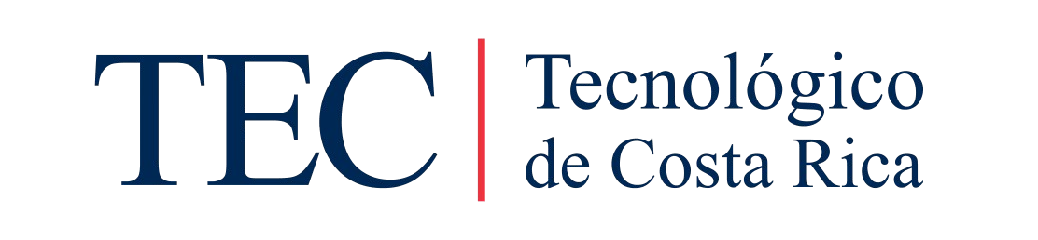
\includegraphics[height=1.5cm]{Images/Tec.png} \hspace{2cm}
    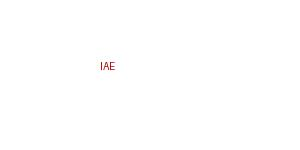
\includegraphics[height=1.5cm]{Images/IAE.jpg}
}

\begin{document}

% ============================================================
% SLIDE 1 -- Title (~15s)
% ============================================================
\begin{frame}
    \titlepage
\end{frame}

% ============================================================
\section{Motivation \& Objectives}
% ============================================================

% SLIDE 2 -- Motivation + all three objectives, one line each (~60s)
\begin{frame}{Motivation \& Objectives}
    \footnotesize
    \textbf{General objective:} characterize MHD oscillations in Heliotron J through
    Python-based analysis, to determine their excitation mechanisms and assess their
    impact on plasma confinement.

    \vspace{0.15cm}
    \textbf{Specific objectives, one shot (\#88653):}
    \begin{enumerate}
        \item \textbf{Spectral properties \& temporal evolution:} identify and validate
        the dominant coherent MHD mode(s) via time-frequency analysis (dual criterion:
        $3\sigma$ amplitude \emph{and} $\gamma^2>0.7$ spatial coherence), determine its
        toroidal number $n$, and localize it radially.
        \item \textbf{EPM--heating correlation:} evaluate the synchronization between
        magnetic fluctuation frequencies and NBI/ECH heating power through statistical
        correlation metrics (envelope vs.\ $I_p$, $W_p$, $n_e$, H$\alpha$; lagged
        cross-correlation), separating Secondary and Primary bands and testing them against
        physical scaling models.
        \item \textbf{Low-frequency H-mode fluctuations \& edge coupling:} map
        non-linear three-wave (bicoherence) and self-coupling of the dominant mode,
        and test its link to edge turbulence modulation and enhanced heat transport,
        under a strict validation criterion.
    \end{enumerate}

    \vspace{0.15cm}
    \textbf{Running thread:} every objective is repeated for the
    \textbf{ECH+NBI} and \textbf{NBI-only} phases of the same discharge, to test
    whether what we find survives the loss of ECH heating.
\end{frame}

% ============================================================
\section{Methodology}
% ============================================================

% SLIDE 3 -- Method in one slide (~45s)
\begin{frame}{Method: Dual-Criterion Validation \& Comparative Windows}
    \begin{itemize}
        \item \textbf{Diagnostics:} toroidal Mirnov array (MP1/MP3/MP4), poloidal
        array (PMP1--PMP14), ECE electron-temperature channels, diamagnetic loop
        ($W_p$), fast H$\alpha$.
        \item \textbf{Time-frequency:} STFT spectrogram + Morlet continuous
        wavelet transform.
        \item \textbf{Dual-criterion gate:} a peak is only accepted as a
        \emph{physical} mode if it clears a $3\sigma$ noise threshold \emph{and}
        shows spatial coherence $\gamma^2>0.7$ on at least one coil pair --
        amplitude alone is never enough.
        \item \textbf{Comparative design:} ECH switches off at $t=\SI{291.3}{ms}$
        in shot \#88653. We compare \textbf{ECH+NBI} (\SIrange{259.1}{291.3}{ms})
        vs.\ \textbf{NBI-only} (\SIrange{291.3}{300.0}{ms}; NBI beams turn off
        at ${\sim}\SI{300.6}{ms}$) -- same shot, same pipeline, run twice,
        isolating the effect of ECH loss.
    \end{itemize}
\end{frame}

% ============================================================
\section{Objective 1: Dominant Mode Identification}
% ============================================================

\begin{frame}{Objective 1: Plasma Heating and Confinement vs.\ Mirnov Signal}
    \begin{figure}[h!]
        \centering
        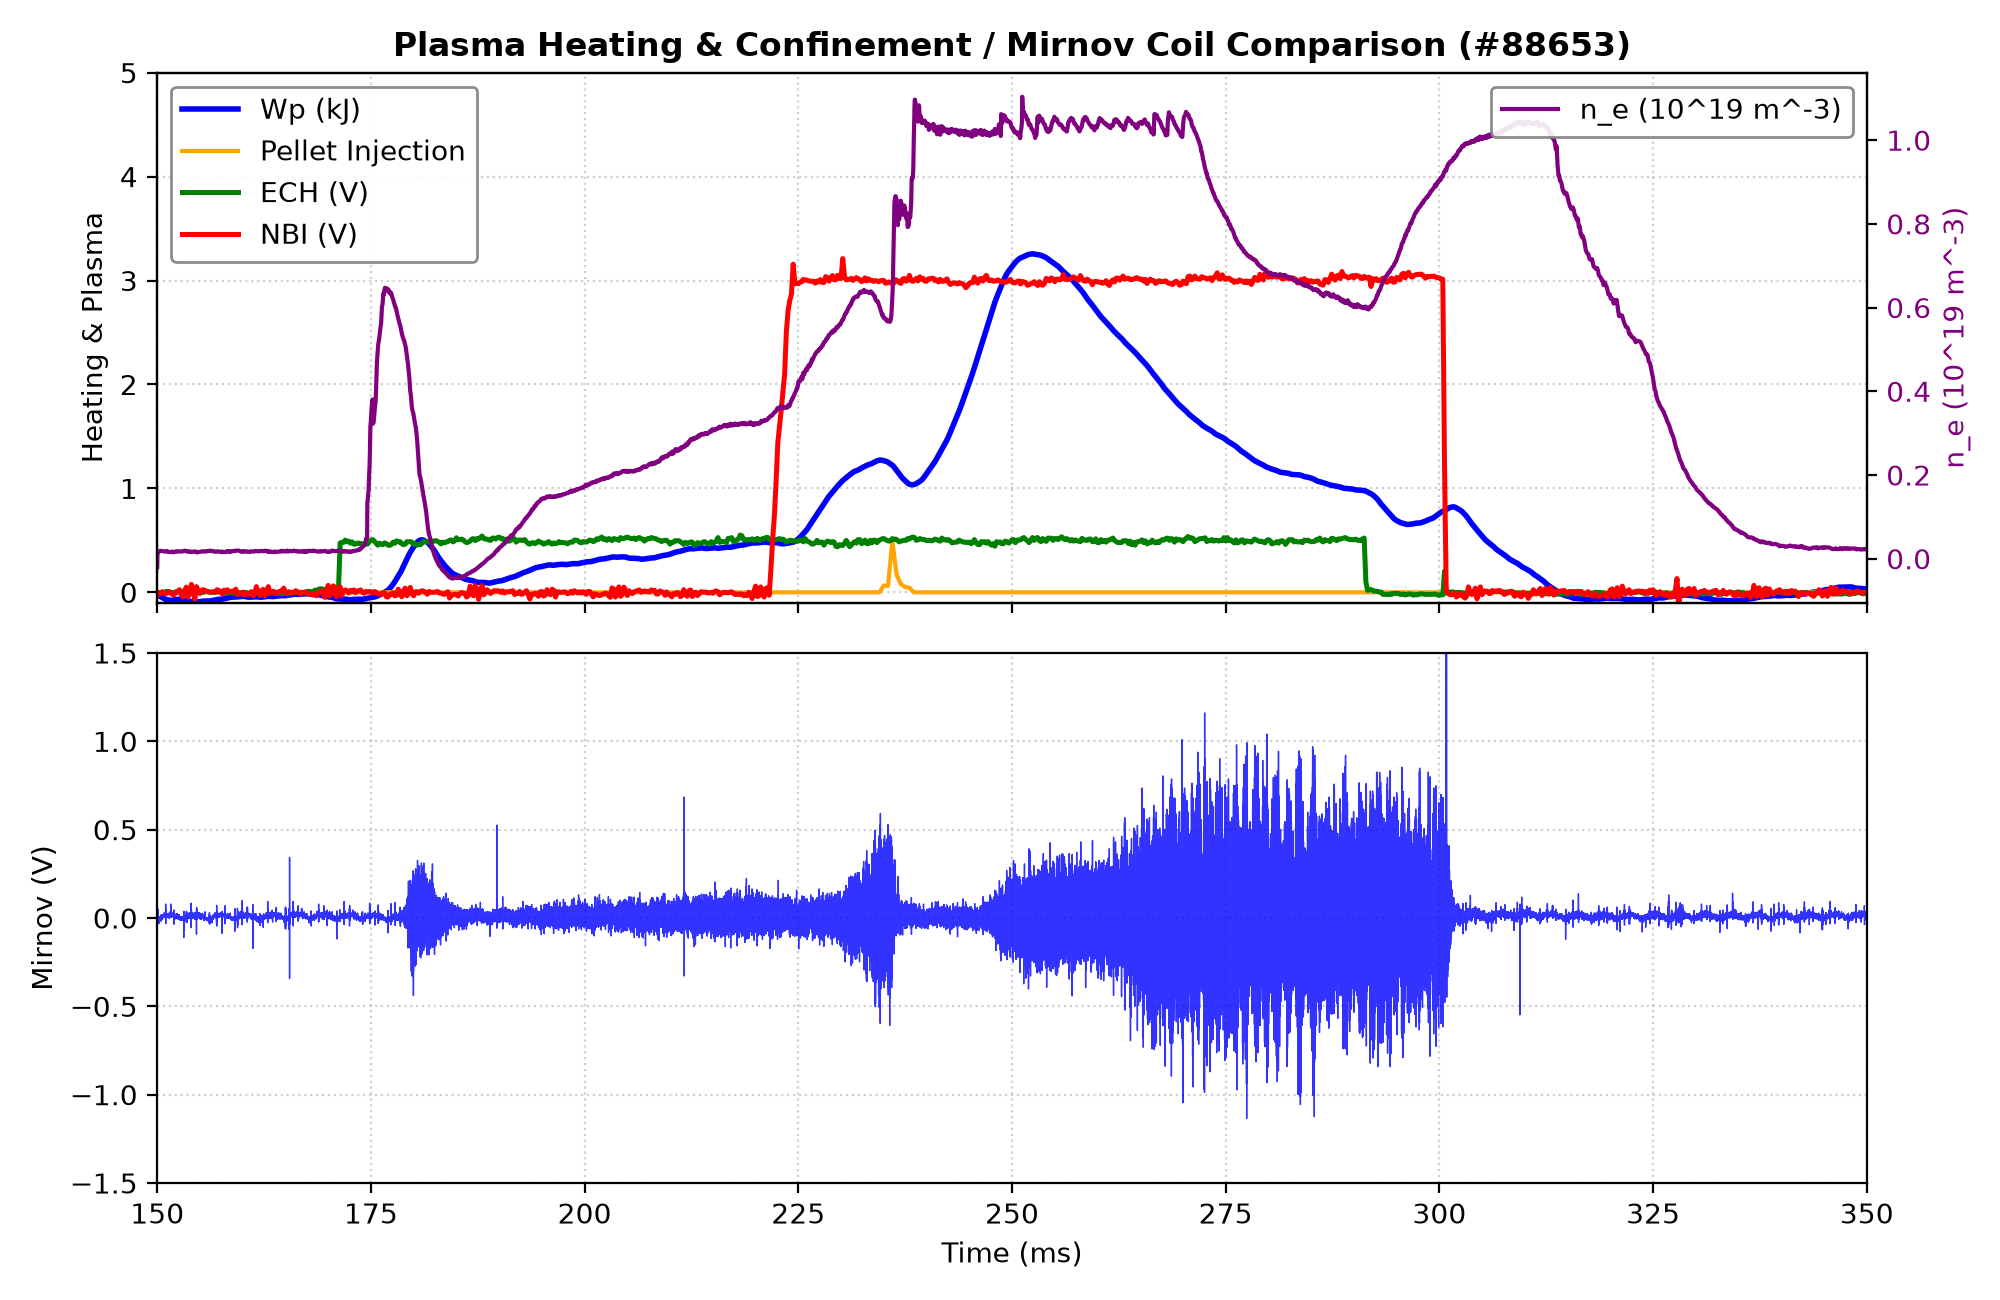
\includegraphics[height=0.85\textheight]{Images/obj2_dynamics_and_structure/heating_vs_mirnov (Shot_88653).png}
    \end{figure}
\end{frame}

\begin{frame}{Objective 1: Spectrogram and Spatial Coherence}
    \begin{figure}[h!]
        \centering
        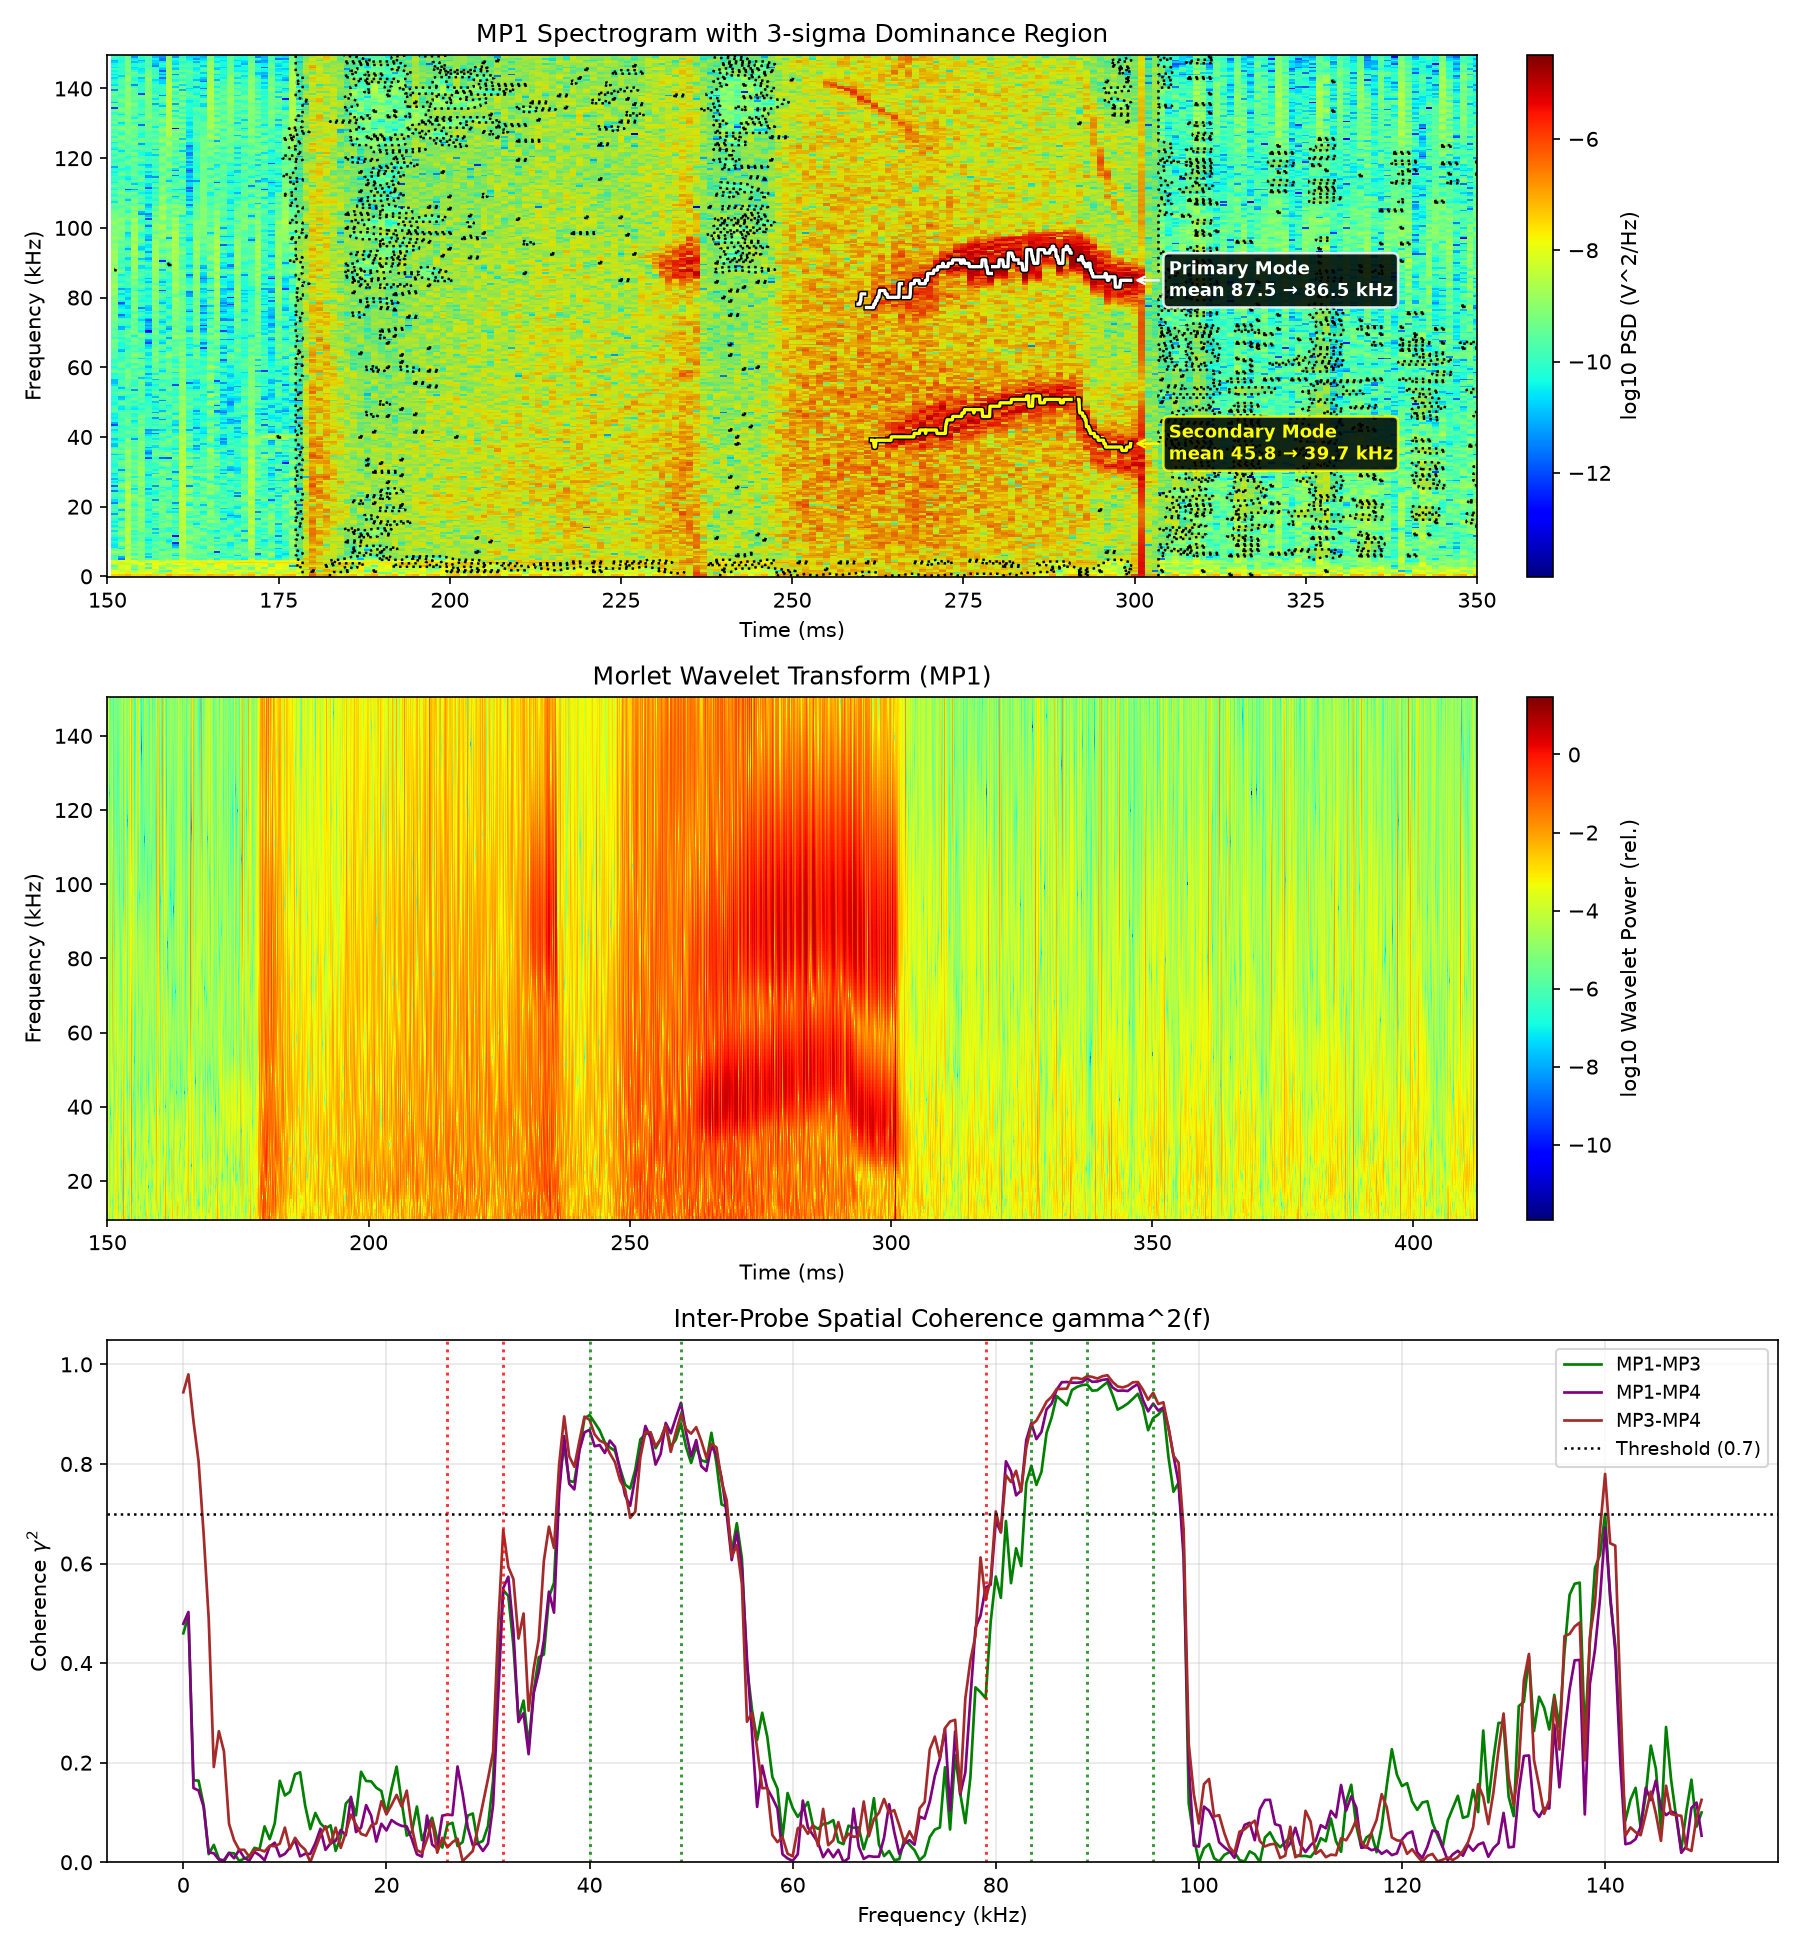
\includegraphics[height=0.85\textheight]{Images/obj1_mode_identification/mhd_analysis_objective1_88653.png}
    \end{figure}
\end{frame}

% SLIDE 4 -- Obj 1 identity result (~90s)
\begin{frame}{Objective 1: A Single, Validated Primary Mode}
    \begin{columns}[c]
        \begin{column}{0.44\textwidth}
            \centering
            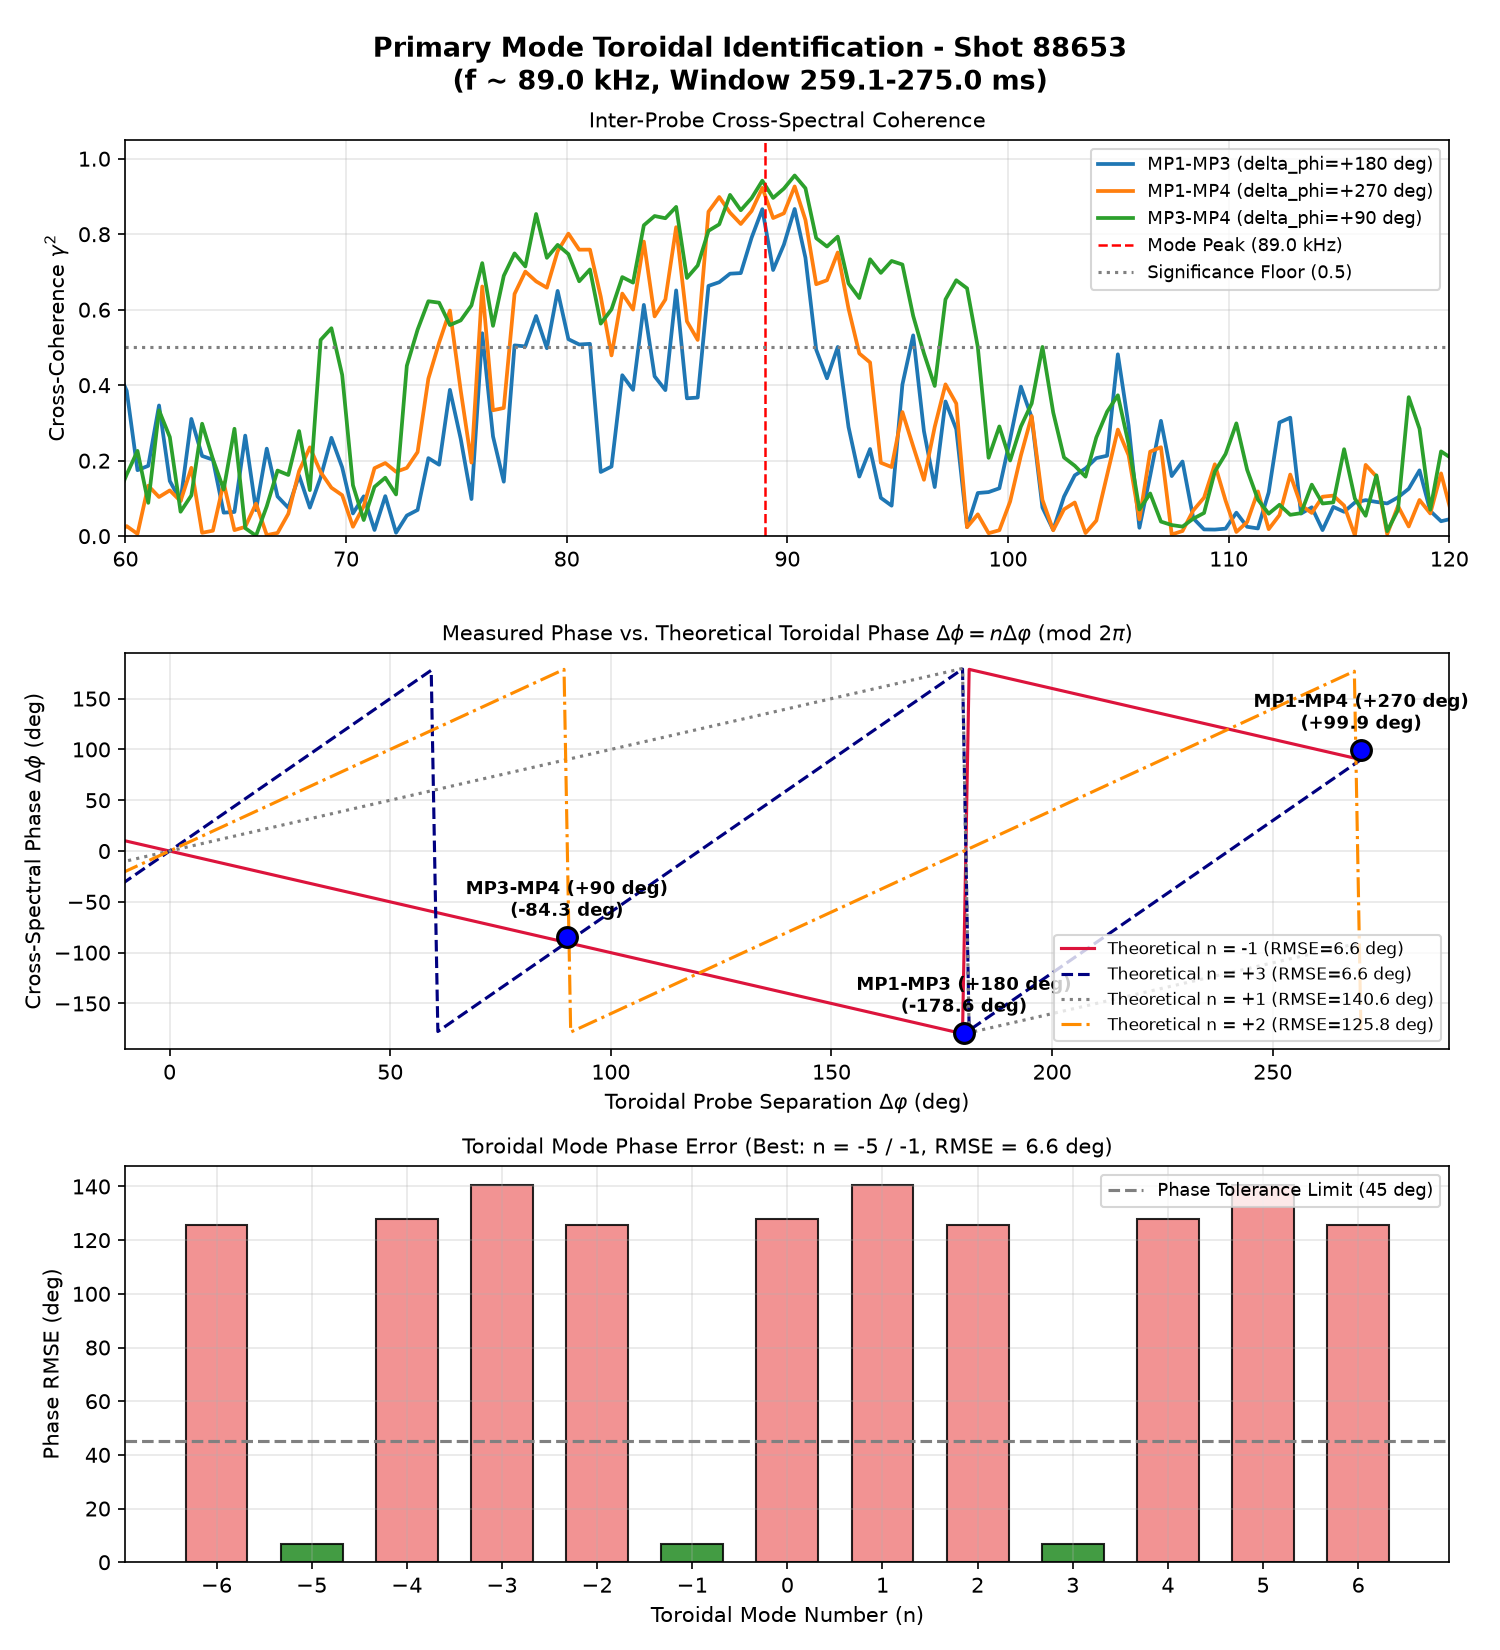
\includegraphics[height=0.84\textheight]{Images/obj1_mode_identification/mhd_primary_mode_toroidal_n_shot_88653.png}
        \end{column}
        \begin{column}{0.54\textwidth}
            \small
            \begin{itemize}
                \item \textbf{89.0 kHz} clears both criteria: $3\sigma$ dominance \emph{and}
                $\gamma^2=0.87$--$0.94$ across all Mirnov pairs (MP1-MP3: 0.87, MP1-MP4: 0.92,
                MP3-MP4: 0.94).
                \item Best-fit toroidal number $n=-5$, RMSE $=\SI{6.6}{\degree}$; with three
                probes only $n\equiv-1$ (mod 4) is determined.
                \item A nearby \SI{95.5}{kHz} peak is most likely the same chirping mode's
                spectral footprint, not a separate instability $\Rightarrow$ treated as
                \textbf{one} primary mode going forward.
            \end{itemize}
        \end{column}
    \end{columns}
\end{frame}

% SLIDE 5 -- Obj 1 spatial localization (~60s)
\begin{frame}{Objective 1: Spatial Structure \& Radial Localization}
    \centering
    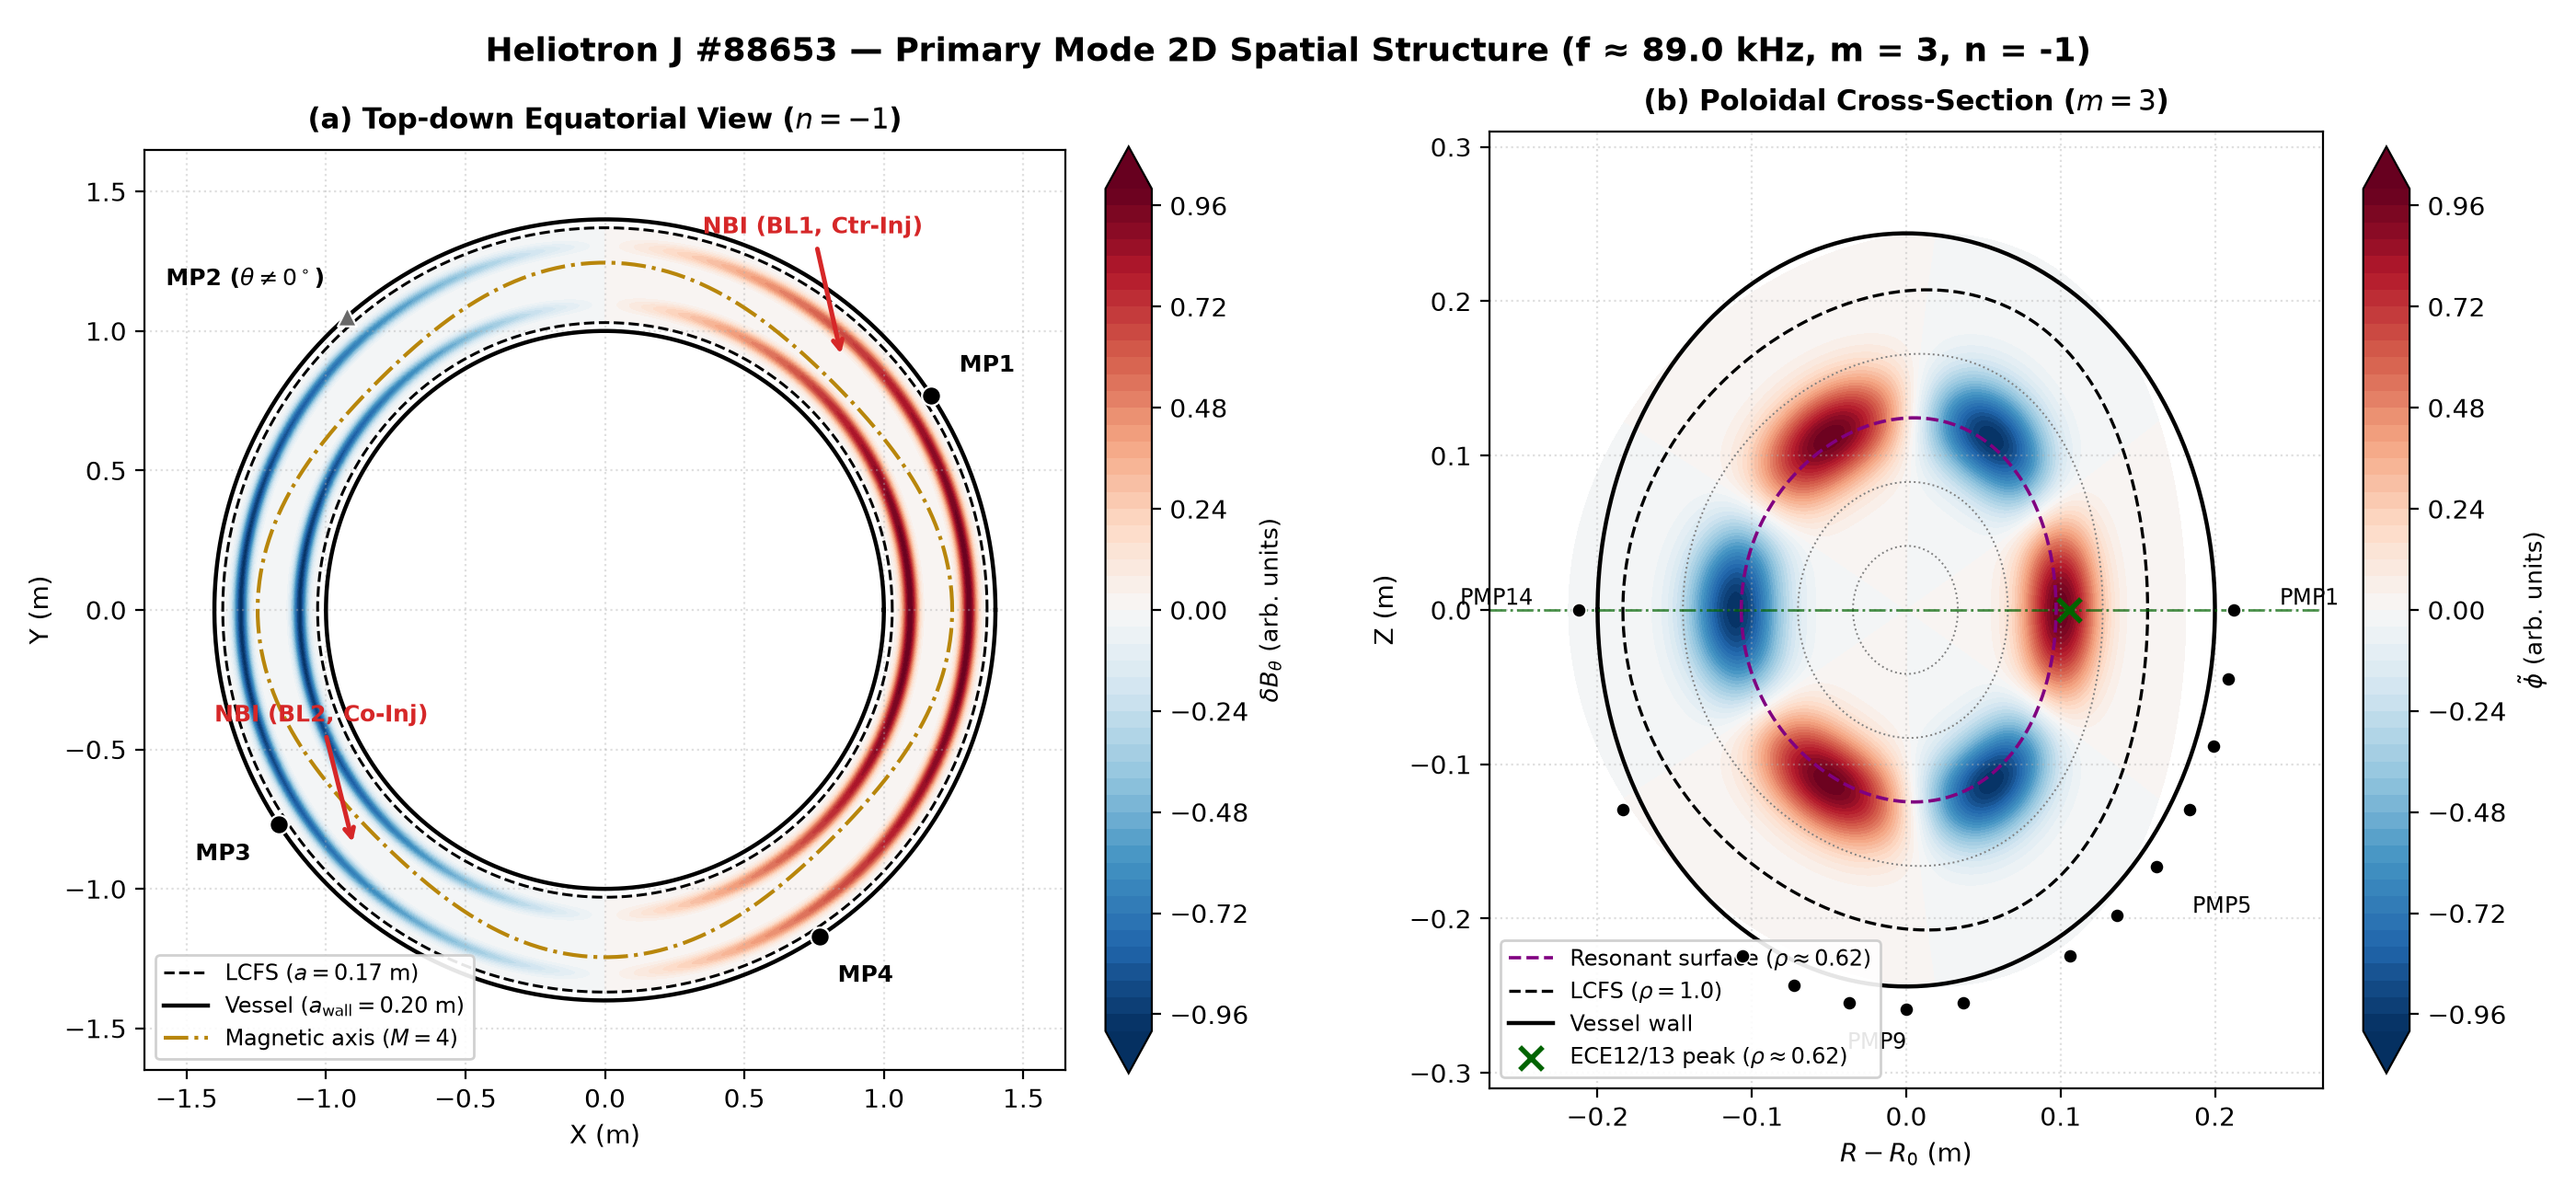
\includegraphics[width=0.62\textwidth]{Images/obj2_dynamics_and_structure/mhd_mode_spatial_map_2d_88653.png}
    \vspace{-0.1cm}
    \footnotesize
    \begin{itemize}
        \item Poloidal number $m=+3$: a single, coherent structure (top-down and poloidal cross-section agree).
        \item ECE fluctuation (\SIrange{80}{100}{kHz}) is largest at ECE12/13FAST
        (\SI{64.5}{GHz}/\SI{66.5}{GHz}; \SI{0.33}{V}/\SI{0.478}{V}, $\sim$200$\times$ the quiet level), near
        $\rho\approx0.62$. ECE12--13 are mutually coherent ($\gamma^2=0.77$) but not with MP1
        ($\gamma^2\approx0.06$ vs.\ floor 0.20): localization is suggestive only.
        \item Weak edge coupling at HAFAST7.5 ($\gamma^2=0.23$: above floor, below 0.7 gate).
    \end{itemize}
\end{frame}

% SLIDE 6 -- Obj 1 comparative persistence (~75s)
\begin{frame}{Objective 1: Mode Identity Survives ECH Shut-off}
    \small
    \centering
    \begin{tabular}{lccccc}
        \toprule
        Window & $f$ (kHz) & $n$ (aliased) & RMSE ($^\circ$) & $\gamma^2$ range \\
        \midrule
        ECH+NBI  & 89.0 & $-5$ ($\equiv -1$) & 5.2 & 0.96--0.98 \\
        NBI-only & 86.0 & $-5$ ($\equiv -1$) & 6.7 & 0.997--0.998 \\
        \bottomrule
    \end{tabular}
    \vspace{0.3cm}
    \normalsize
    \begin{itemize}
        \item The \textbf{same toroidal number and helicity} persist after ECH
        shuts off; only the frequency downshifts ($\sim$2--\SI{3}{kHz} primary: PSD peak
        89.0$\to$87.0, $n$-fit line 89.0$\to$86.0; $\sim$\SI{11.5}{kHz} secondary) -- consistent with electron
        cooling (lower sound speed) or a rotation/Doppler shift.
        \item In both windows $3\sigma$ occupancy is 100\%: the mode is
        \textbf{continuously sustained} by the NBI fast-ion drive, not decaying --
        but it hops discretely among 2--3 frequency branches
        ($\sim$0.4--1.3 jumps/ms), a hallmark of EPM/BAE avalanche (hole-clump)
        dynamics.
        \item \textbf{Reproduces in an independent shot:} validation shot
        \#88654 shows the same mode structure -- same rank order,
        comparable amplitudes, comparable or higher coherence -- downshifted
        $\sim$1--\SI{2.5}{kHz} (backup).
    \end{itemize}
\end{frame}

% ============================================================
\section{Objective 2: Spatial Structure \& Dynamics}
% ============================================================

% SLIDE 7 -- Obj 2 dual-band scaling (~90s)
\begin{frame}{Objective 2: Two Bands -- Poloidal Structure and Scaling Tests}
    \begin{columns}[c]
        \begin{column}{0.36\textwidth}
            \centering
            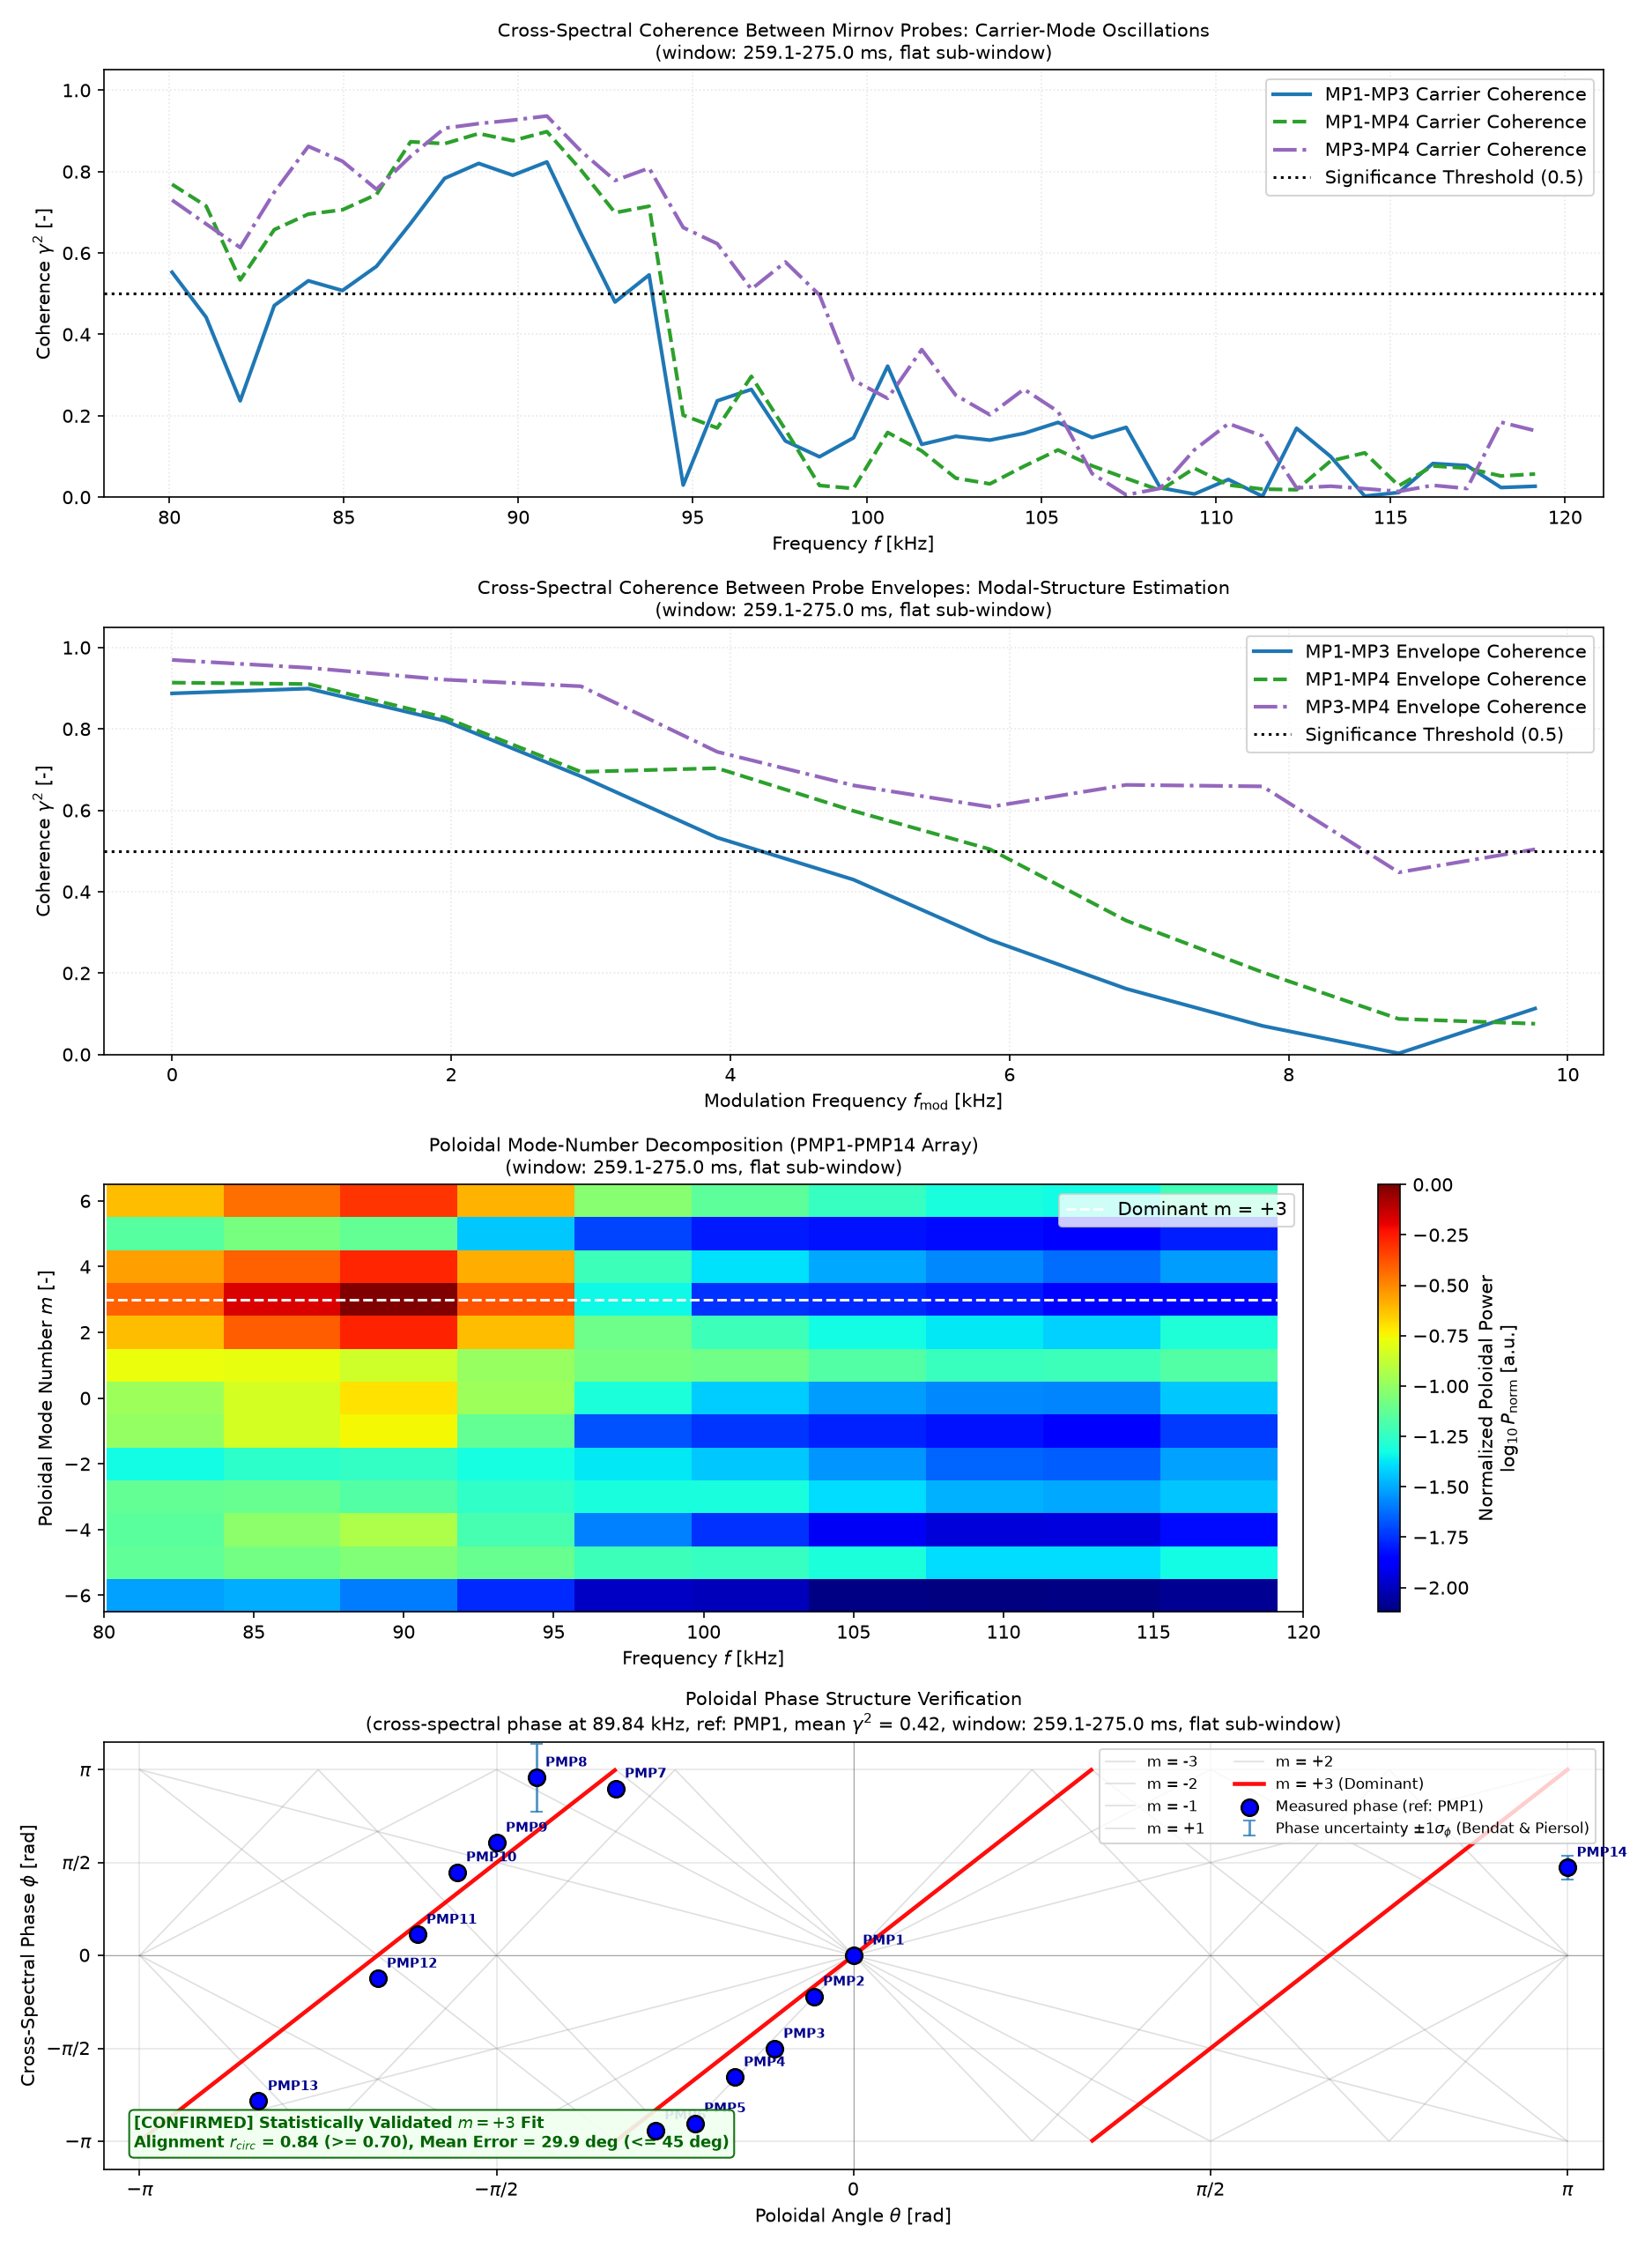
\includegraphics[height=0.84\textheight]{Images/obj2_dynamics_and_structure/mhd_analysis_objective2_structure_88653_80_120kHz.png}
        \end{column}
        \begin{column}{0.62\textwidth}
            \small
            \begin{itemize}
                \item \textbf{Primary (\SIrange{80}{120}{kHz}):} $m=+3$ \textbf{confirmed} in both windows
                ($r_{\text{circ}}$ up to 0.90), $f=\SI{89.84}{kHz}$; highest-$|r|$ scaling model
                BAE/GAM ($\sqrt{T_e}$): $r=-0.48$ ($p=0.20$).
                \item \textbf{Secondary (\SIrange{40}{80}{kHz}):} $m$ tentative ($+6\to+2$ between
                windows; $r_{\text{circ}}<0.7$), $f=\SI{42.97}{kHz}$; highest-$|r|$ model
                current-induced ($I_p$): $r=-0.85$ ($p=0.16$).
                \item \textbf{Scaling tests:} none of six models is significant
                (adjusted $p>0.16$; $N_{\text{eff}}\approx4$ for Secondary, $\approx9$ for Primary), and both
                top-$|r|$ models have the sign opposite to their prediction -- no model is identified.
            \end{itemize}
        \end{column}
    \end{columns}
\end{frame}

% SLIDE 8 -- Obj 2 macroscopic + heating correlations (~60s)
\begin{frame}{Objective 2: EPM--Heating Statistical Correlation Metrics}
    \small
    \begin{center}
    \begin{tabular}{lcc}
        \toprule
        Correlation with mode envelope & Secondary band ($r$) & Primary band ($r$) \\
        \midrule
        Plasma current $I_p$        & 0.801 & 0.758 \\
        Stored energy $W_p$         & 0.810 & 0.784 \\
        Line-averaged density $n_e$ ($t\ge270$\,ms) & 0.874 & 0.867 \\
        Fast H$\alpha$ emission     & 0.609 & 0.568 \\
        \midrule
        NBI power (direct)          & $\sim$0.61--0.64 & $\sim$0.61--0.64 \\
        ECH power (direct)          & $\sim$0.44--0.45 & $\sim$0.44--0.45 \\
        ECH power (\emph{partial}, step removed) & 0.06--0.12 & 0.06--0.12 \\
        \bottomrule
    \end{tabular}
    \end{center}
    \vspace{0.3cm}
    \normalsize
    Once the shared ECH-on/off step is partialled out, the ECH correlation nearly
    vanishes while the NBI correlation survives $\Rightarrow$ consistent with
    drive by the \textbf{NBI fast-ion population} rather than ECH. Caveat: NBI
    is also an on/off step shared with all plasma signals, and $I_p$, $W_p$,
    $n_e$ correlate more strongly (0.76--0.87); the series are strongly
    autocorrelated, so the correlations are descriptive, not tests.
\end{frame}

% SLIDE 9 -- Obj 2 self-coupling (~75s)
\begin{frame}{Objective 2: The Carrier Talks to Its Own Envelope}
    \begin{columns}[c]
        \begin{column}{0.58\textwidth}
            \centering
            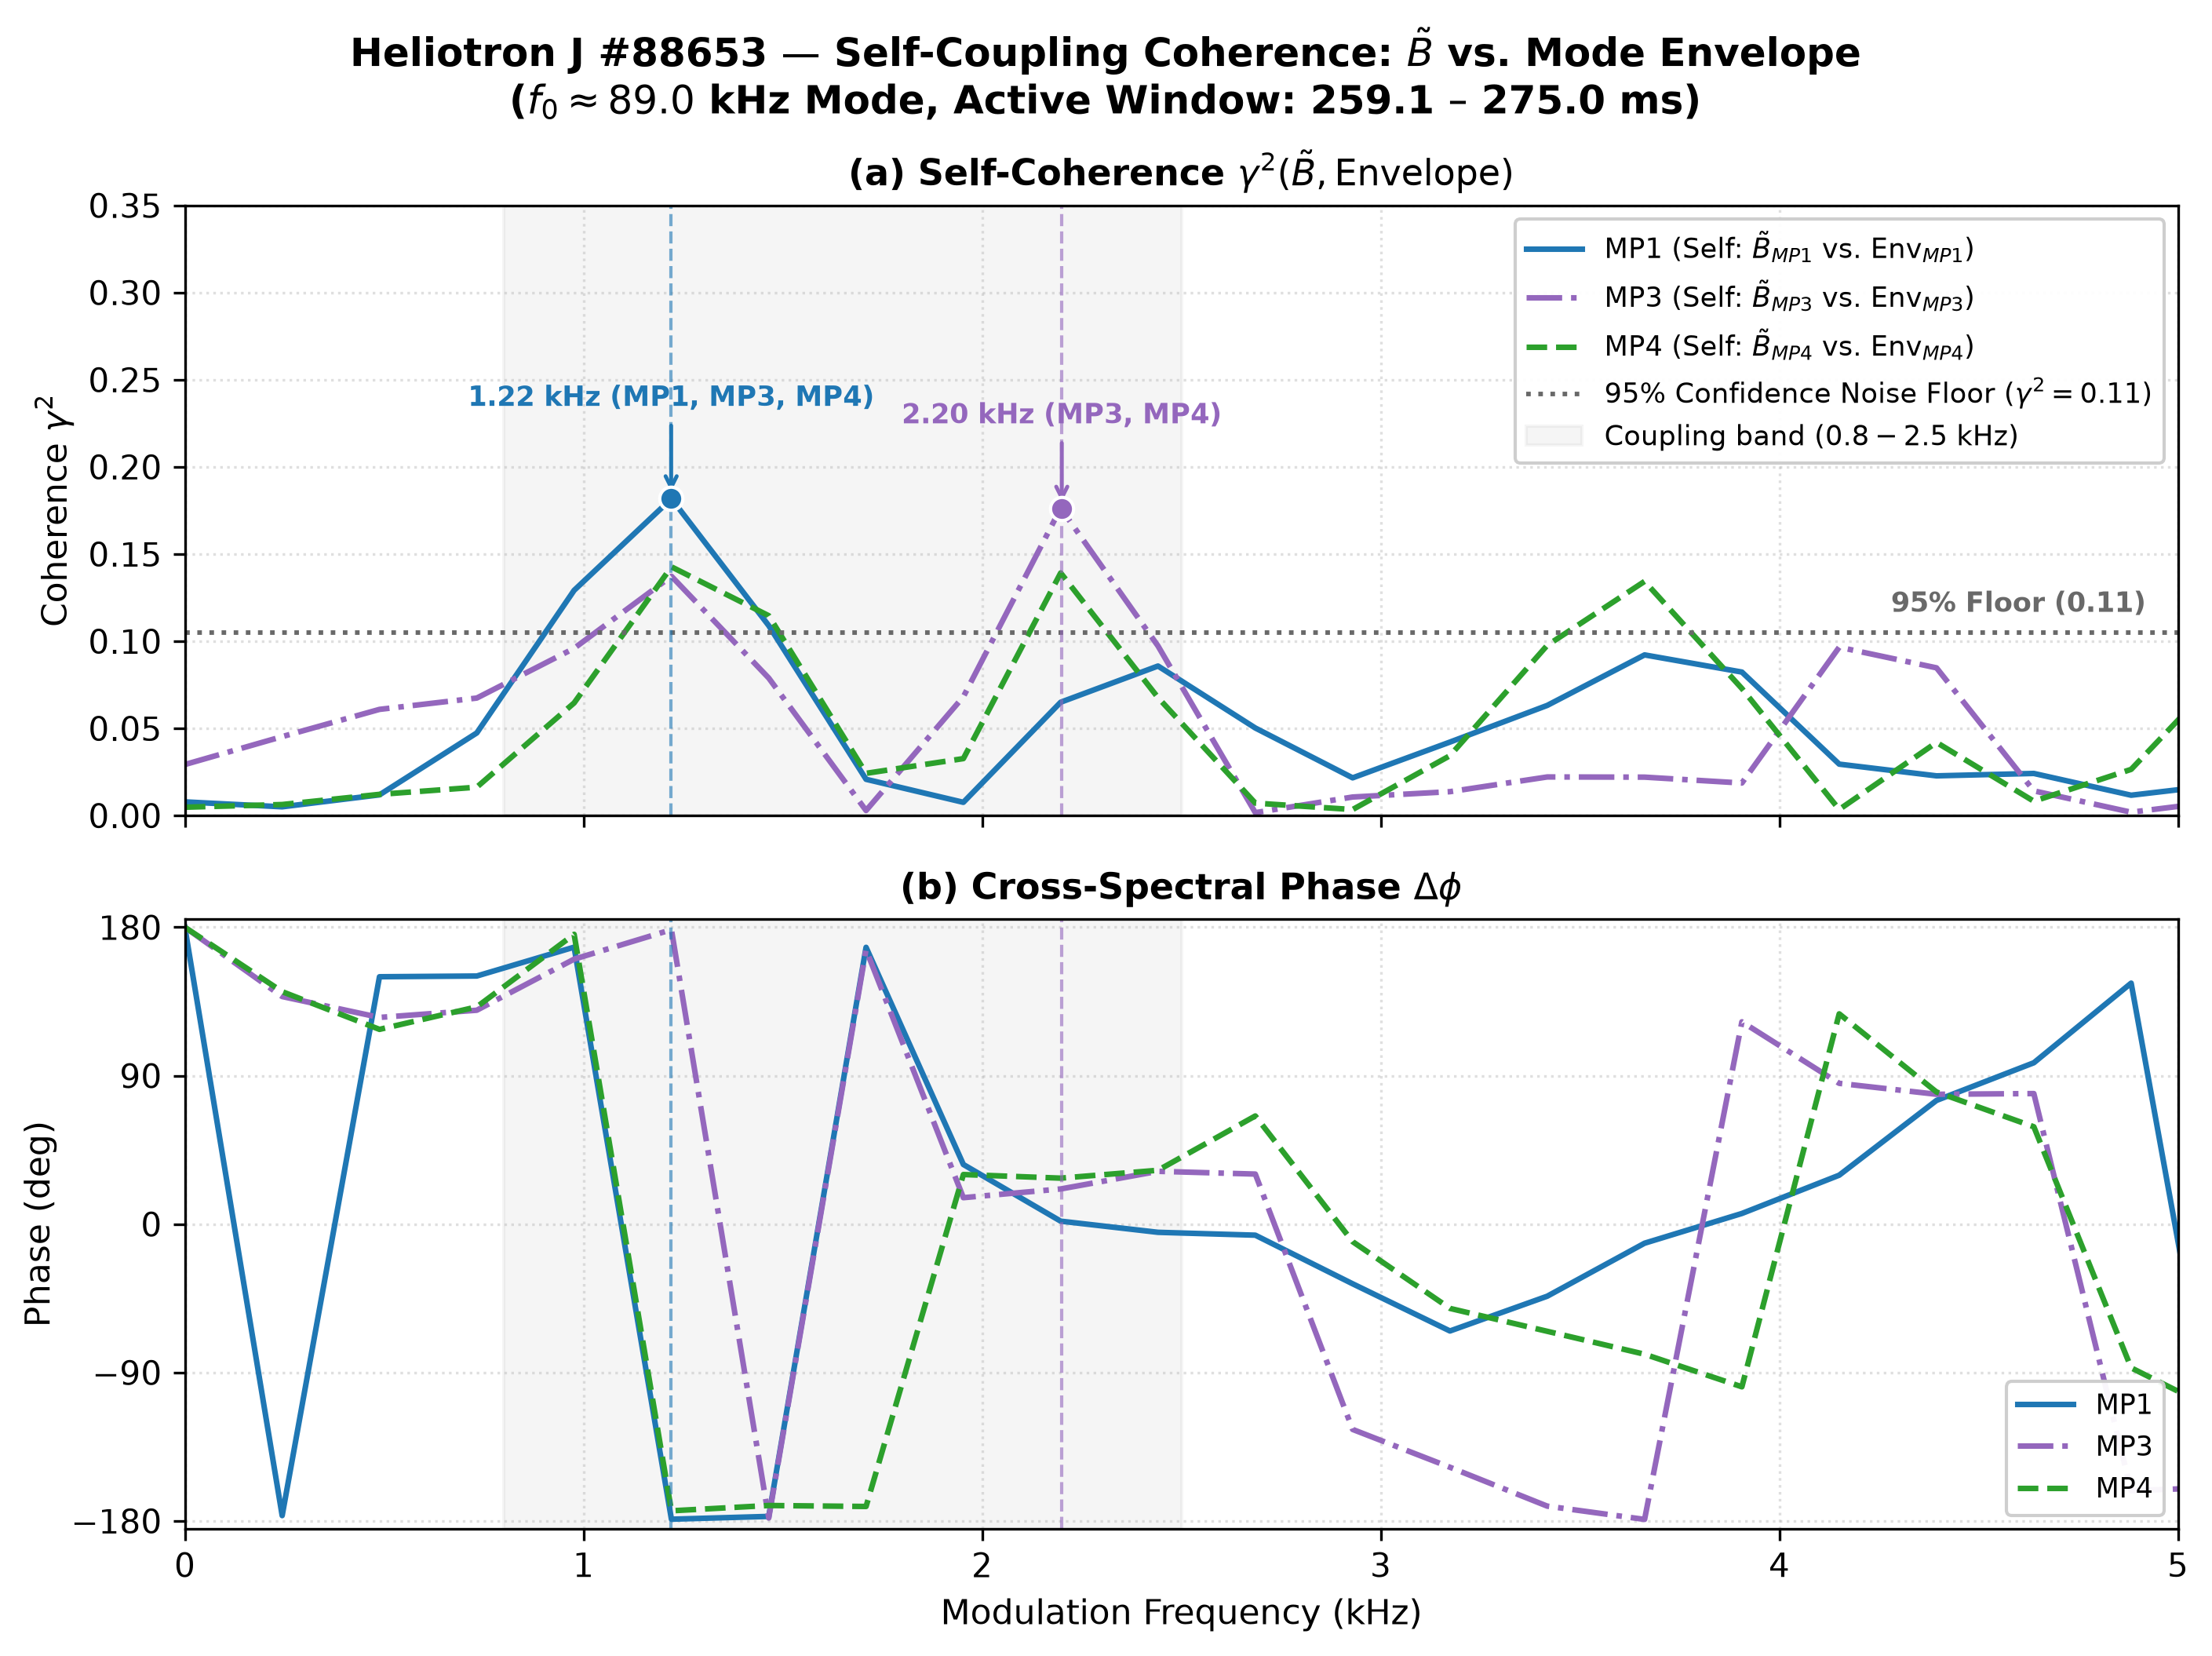
\includegraphics[width=\textwidth]{Images/obj2_dynamics_and_structure/mhd_self_coupling_coherence_shot_88653.png}
        \end{column}
        \begin{column}{0.40\textwidth}
            \footnotesize
            \begin{itemize}
                \item Self-coherence $\gamma^2$ of $\tilde{B}$ with its own Hilbert envelope
                peaks near \SI{1.2}{kHz} (all three probes: MP1 0.18, MP3/MP4 0.14) and
                \SI{2.2}{kHz} (MP3 0.18, MP4 0.14; MP1 below floor), above the
                nominal 95\% floor of 0.105 (\SIrange{259.1}{275.0}{ms}; segment overlap makes
                the floor optimistic).
                \item The \SI{2.2}{kHz} peak (MP3, MP4) persists at 2$\times$ and 4$\times$
                resolution and exceeds the floor in all three probes in the NBI-only window; the
                \SI{1.2}{kHz} peak already clears the floor on all three probes here, strongest
                on MP1.
                \item Consistent with a weak wave--envelope interaction (linear beating of
                adjacent lines also gives envelope coherence); motivation for Objective 3.
            \end{itemize}
        \end{column}
    \end{columns}
\end{frame}

% ============================================================
\section{Objective 3: Non-linear Coupling (Bicoherence)}
% ============================================================

% SLIDE 10 -- Obj 3 discovery (~90s)
\begin{frame}{Objective 3: A Striking $f \leftrightarrow f/2$ Locking Signature}
    \centering
    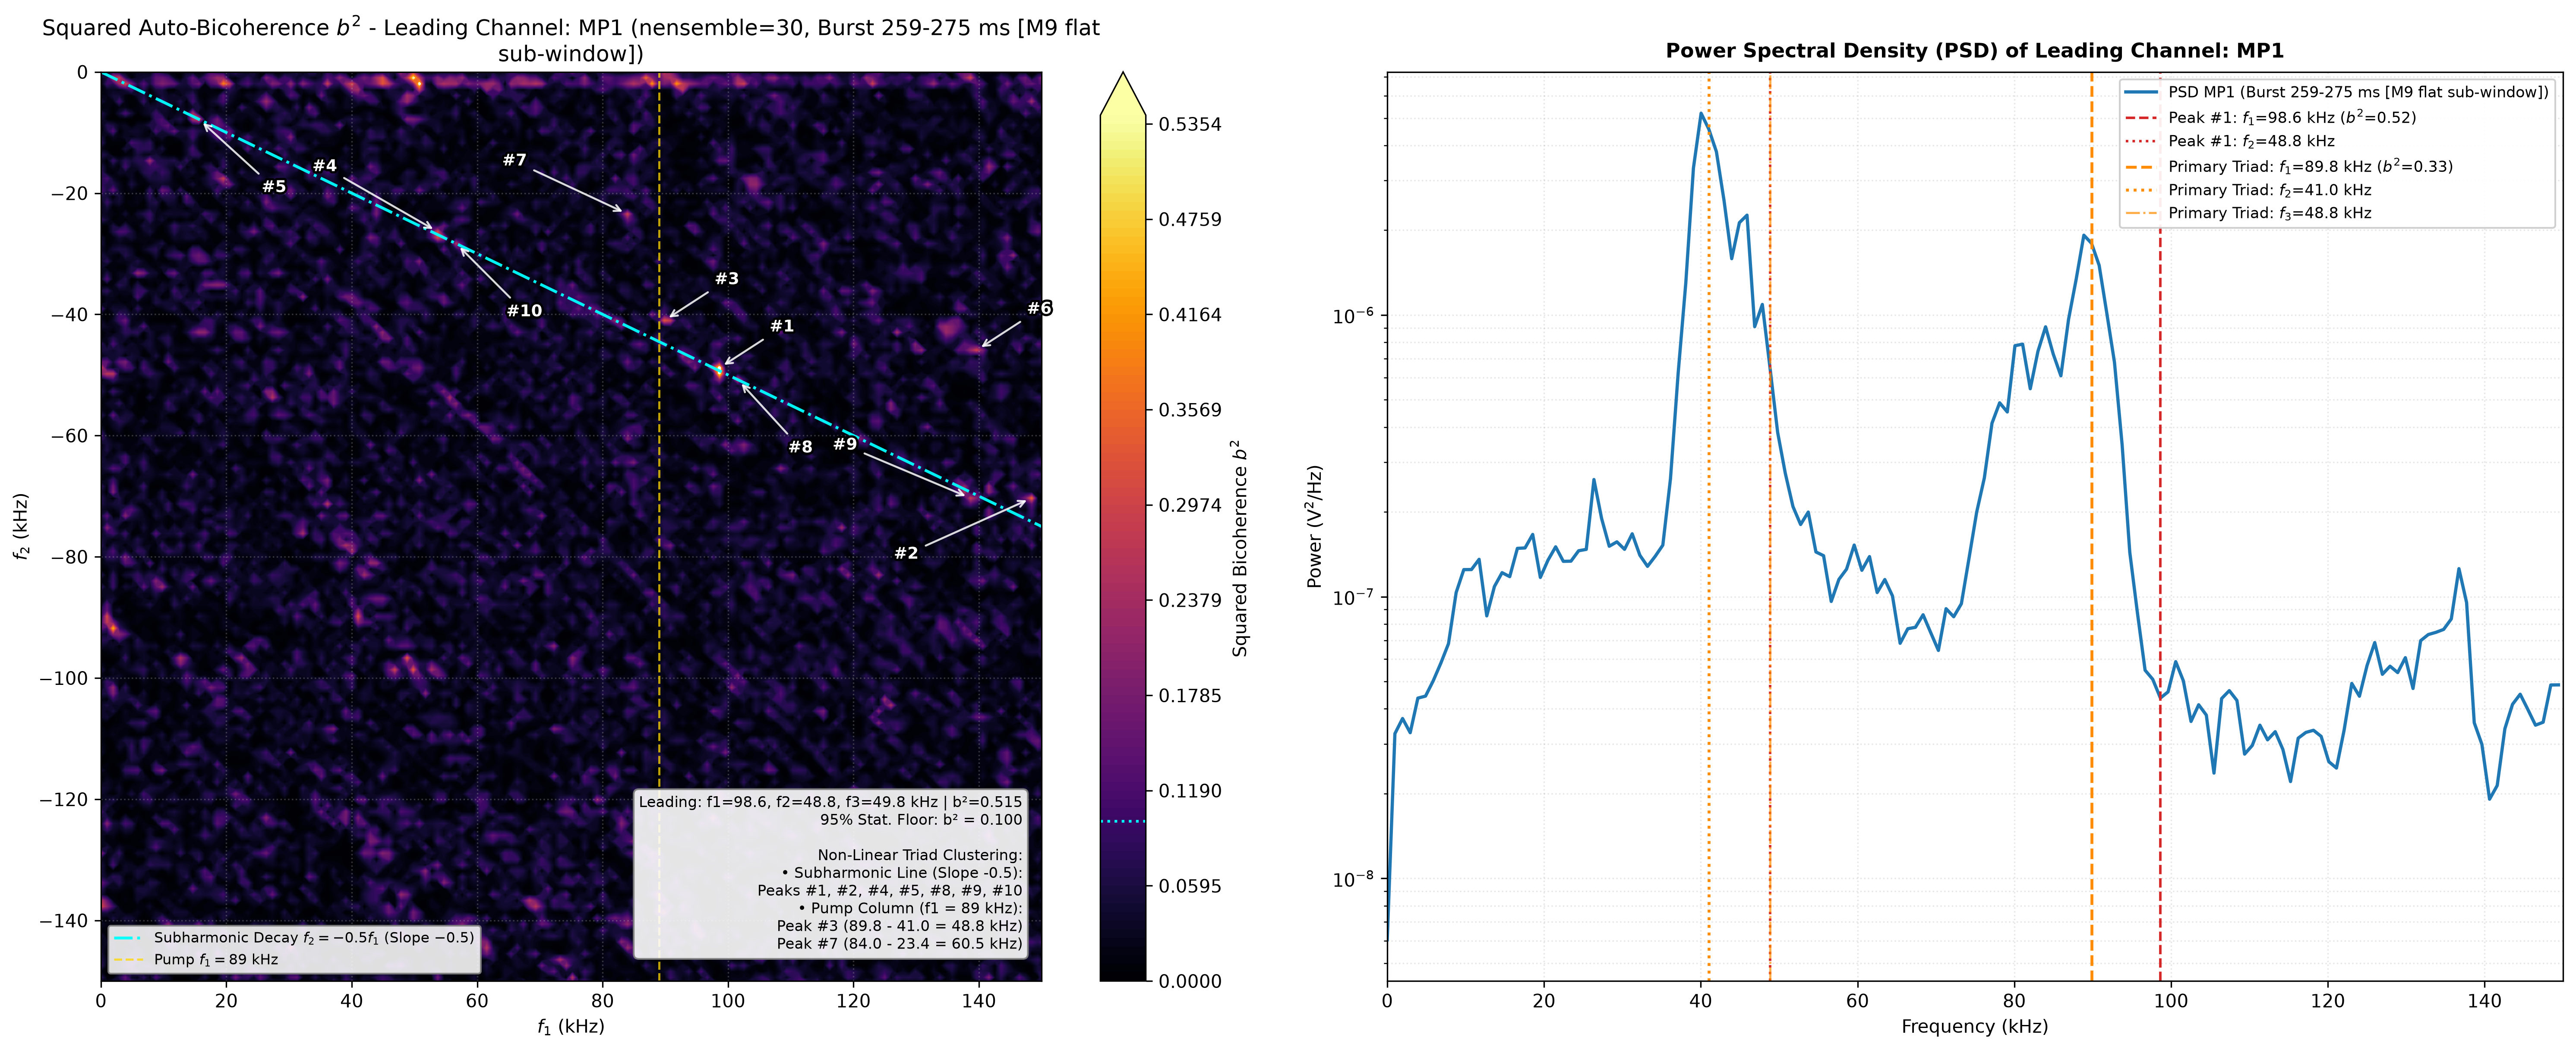
\includegraphics[width=0.95\textwidth]{Images/obj3_nonlinear_coupling/mhd_bicoherence_objective3_88653.png}
    \vspace{-0.05cm}
    \footnotesize
    \raggedright
    MP1 auto-bicoherence (\SIrange{259.1}{275.0}{ms}) peaks at $b^2=0.515$ for
    $f_1=\SI{98.6}{kHz}$, $f_2=\SI{-48.8}{kHz}$, with leading triads along $f_2\approx-0.5f_1$:
    $f_3=f_1-0.5f_1=0.5f_1\Rightarrow|f_2|=|f_3|=\tfrac12f_1$, an
    $f\leftrightarrow f/2$ phase lock (ratio 0.495). Caveat: $b^2=0.515$ is comparable to
    quiet-time maxima (0.35--0.69); the strongest ridge ($b^2=0.88$) is in the NBI-only window, and
    later windows shift to asymmetric triads.
\end{frame}

% SLIDE 11 -- Obj 3 energy-transfer direction (NEW) (~80s)
\begin{frame}{Objective 3: Energy Transfer Is Upward in the Strongest Windows}
    \begin{columns}[T]
        \begin{column}{0.52\textwidth}
            \centering
            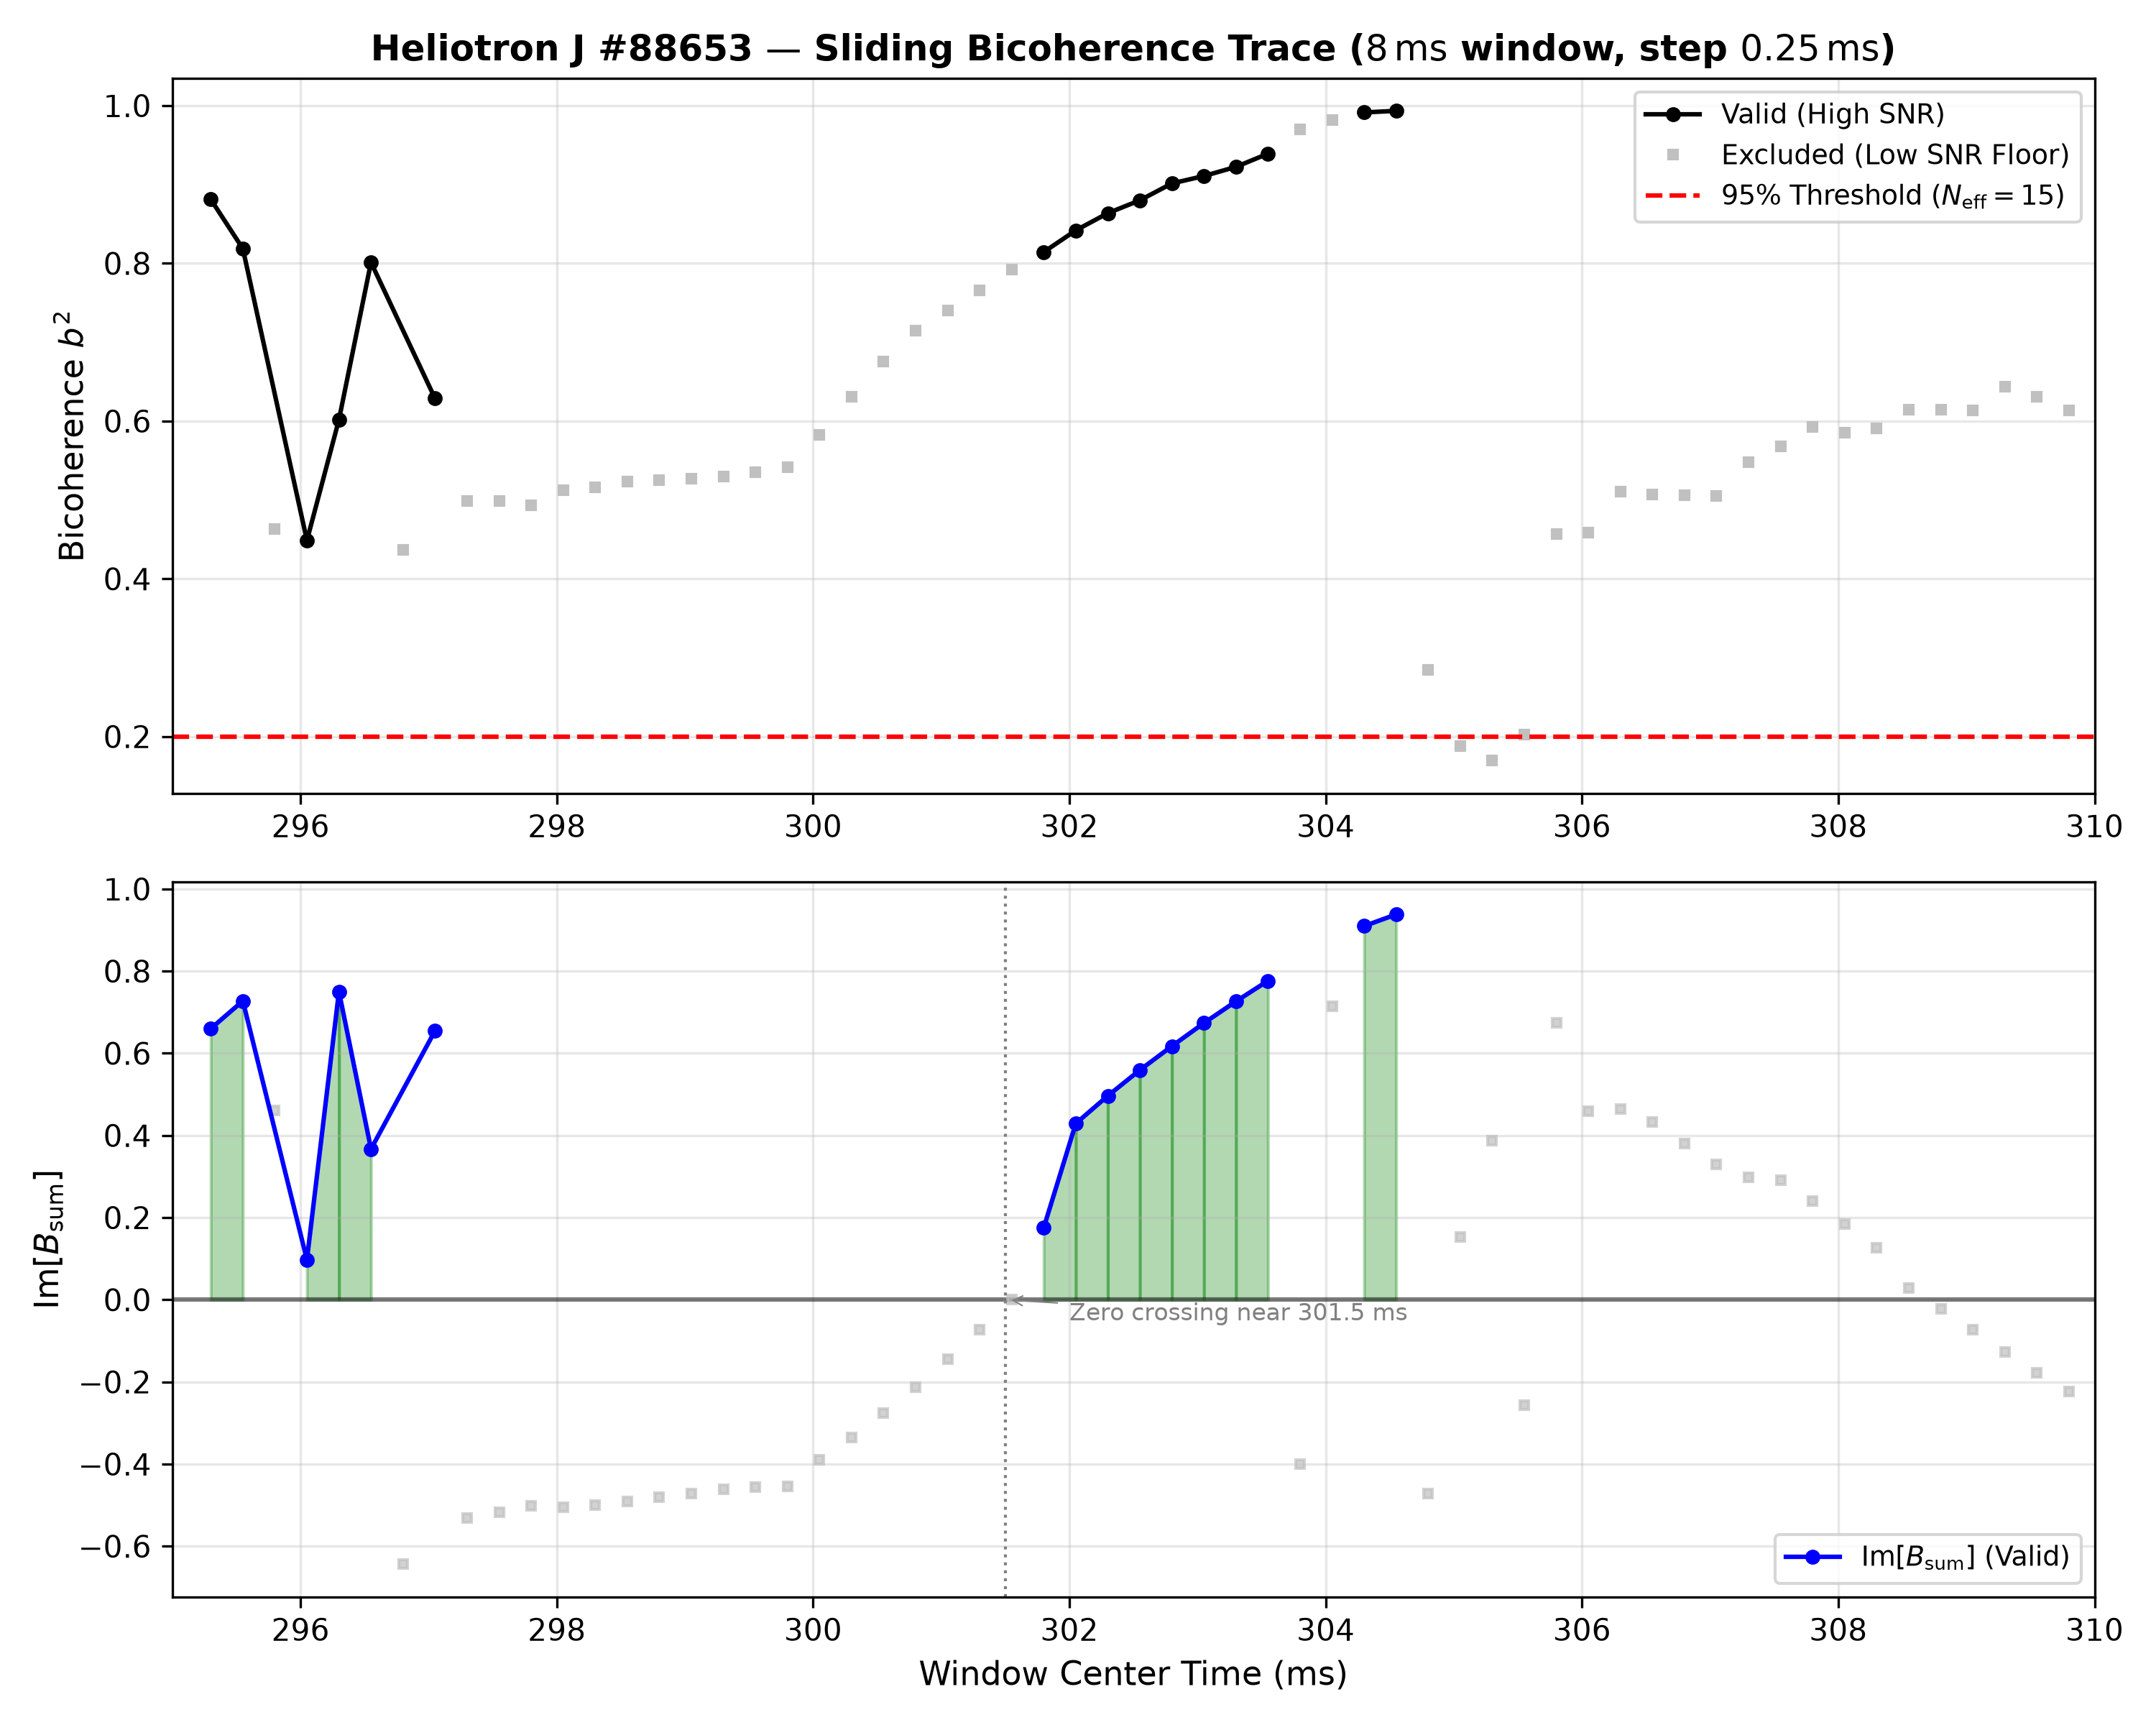
\includegraphics[width=\textwidth]{Images/heating_phase_comparison/bicoherence_sliding_trace_snr.png}
        \end{column}
        \begin{column}{0.48\textwidth}
            \scriptsize
            \begin{itemize}
                \item The \textbf{sign} of $\mathrm{Im}[B_{\text{sum}}]$ sets the
                direction: $>0$ = \textbf{coalescence} (up); $<0$ = decay (down).
                \item Episode 1 (6 windows, centers \SIrange{295.3}{297.1}{ms}; 5 end
                before the $\sim$\SI{300.6}{ms} beam turn-off, 1 straddles it) is near
                $f/2$ in 4 of 6 ($47+98\to145$\,kHz in two). Episode 2 (10 windows,
                \SIrange{301.8}{304.6}{ms}, all straddling turn-off): 0 of 10 near
                $f/2$; the triads change (e.g.\ $44.9+66.4\to111.3$\,kHz in 5 windows).
                \item All 16 windows with $\mathrm{den}>2.5\times10^{-23}$ have
                $\mathrm{Im}[B_{\text{sum}}]>0$ (16/16 for
                $2.5$--$4.0\times10^{-23}$; 17/18 at $2.0$; 18/22 at $1.5\times10^{-23}$).
                \item Windows below the cut at \SIrange{296.8}{301.5}{ms} (grey,
                $b^2\approx0.4$--$0.8$) have $\mathrm{Im}<0$, rising smoothly through
                zero near \SI{301.5}{ms}: the biphase drifts, so the sign is
                \emph{threshold-dependent}.
                \item 97\% window overlap $\Rightarrow$ $\sim$2 independent episodes.
            \end{itemize}
            \vspace{0.1cm}
            \tiny $b^2$ is a maximum over many bins (per-bin 95\% level: 0.20 for
            $N_{\text{eff}}=15$). In 18 quiet-time windows ($\sim$2 independent) the
            maximum $b^2$ was 0.35--0.69; 15 of 16 valid windows exceed 0.69.
        \end{column}
    \end{columns}
\end{frame}

% SLIDE 12 -- Obj 3 mode identity & burst dynamics (NEW) (~85s)
\begin{frame}{Objective 3: Which Mode Drives Which? Inconclusive}
    \begin{columns}
        \begin{column}{0.42\textwidth}
            \begin{figure}[h!]
                \centering
                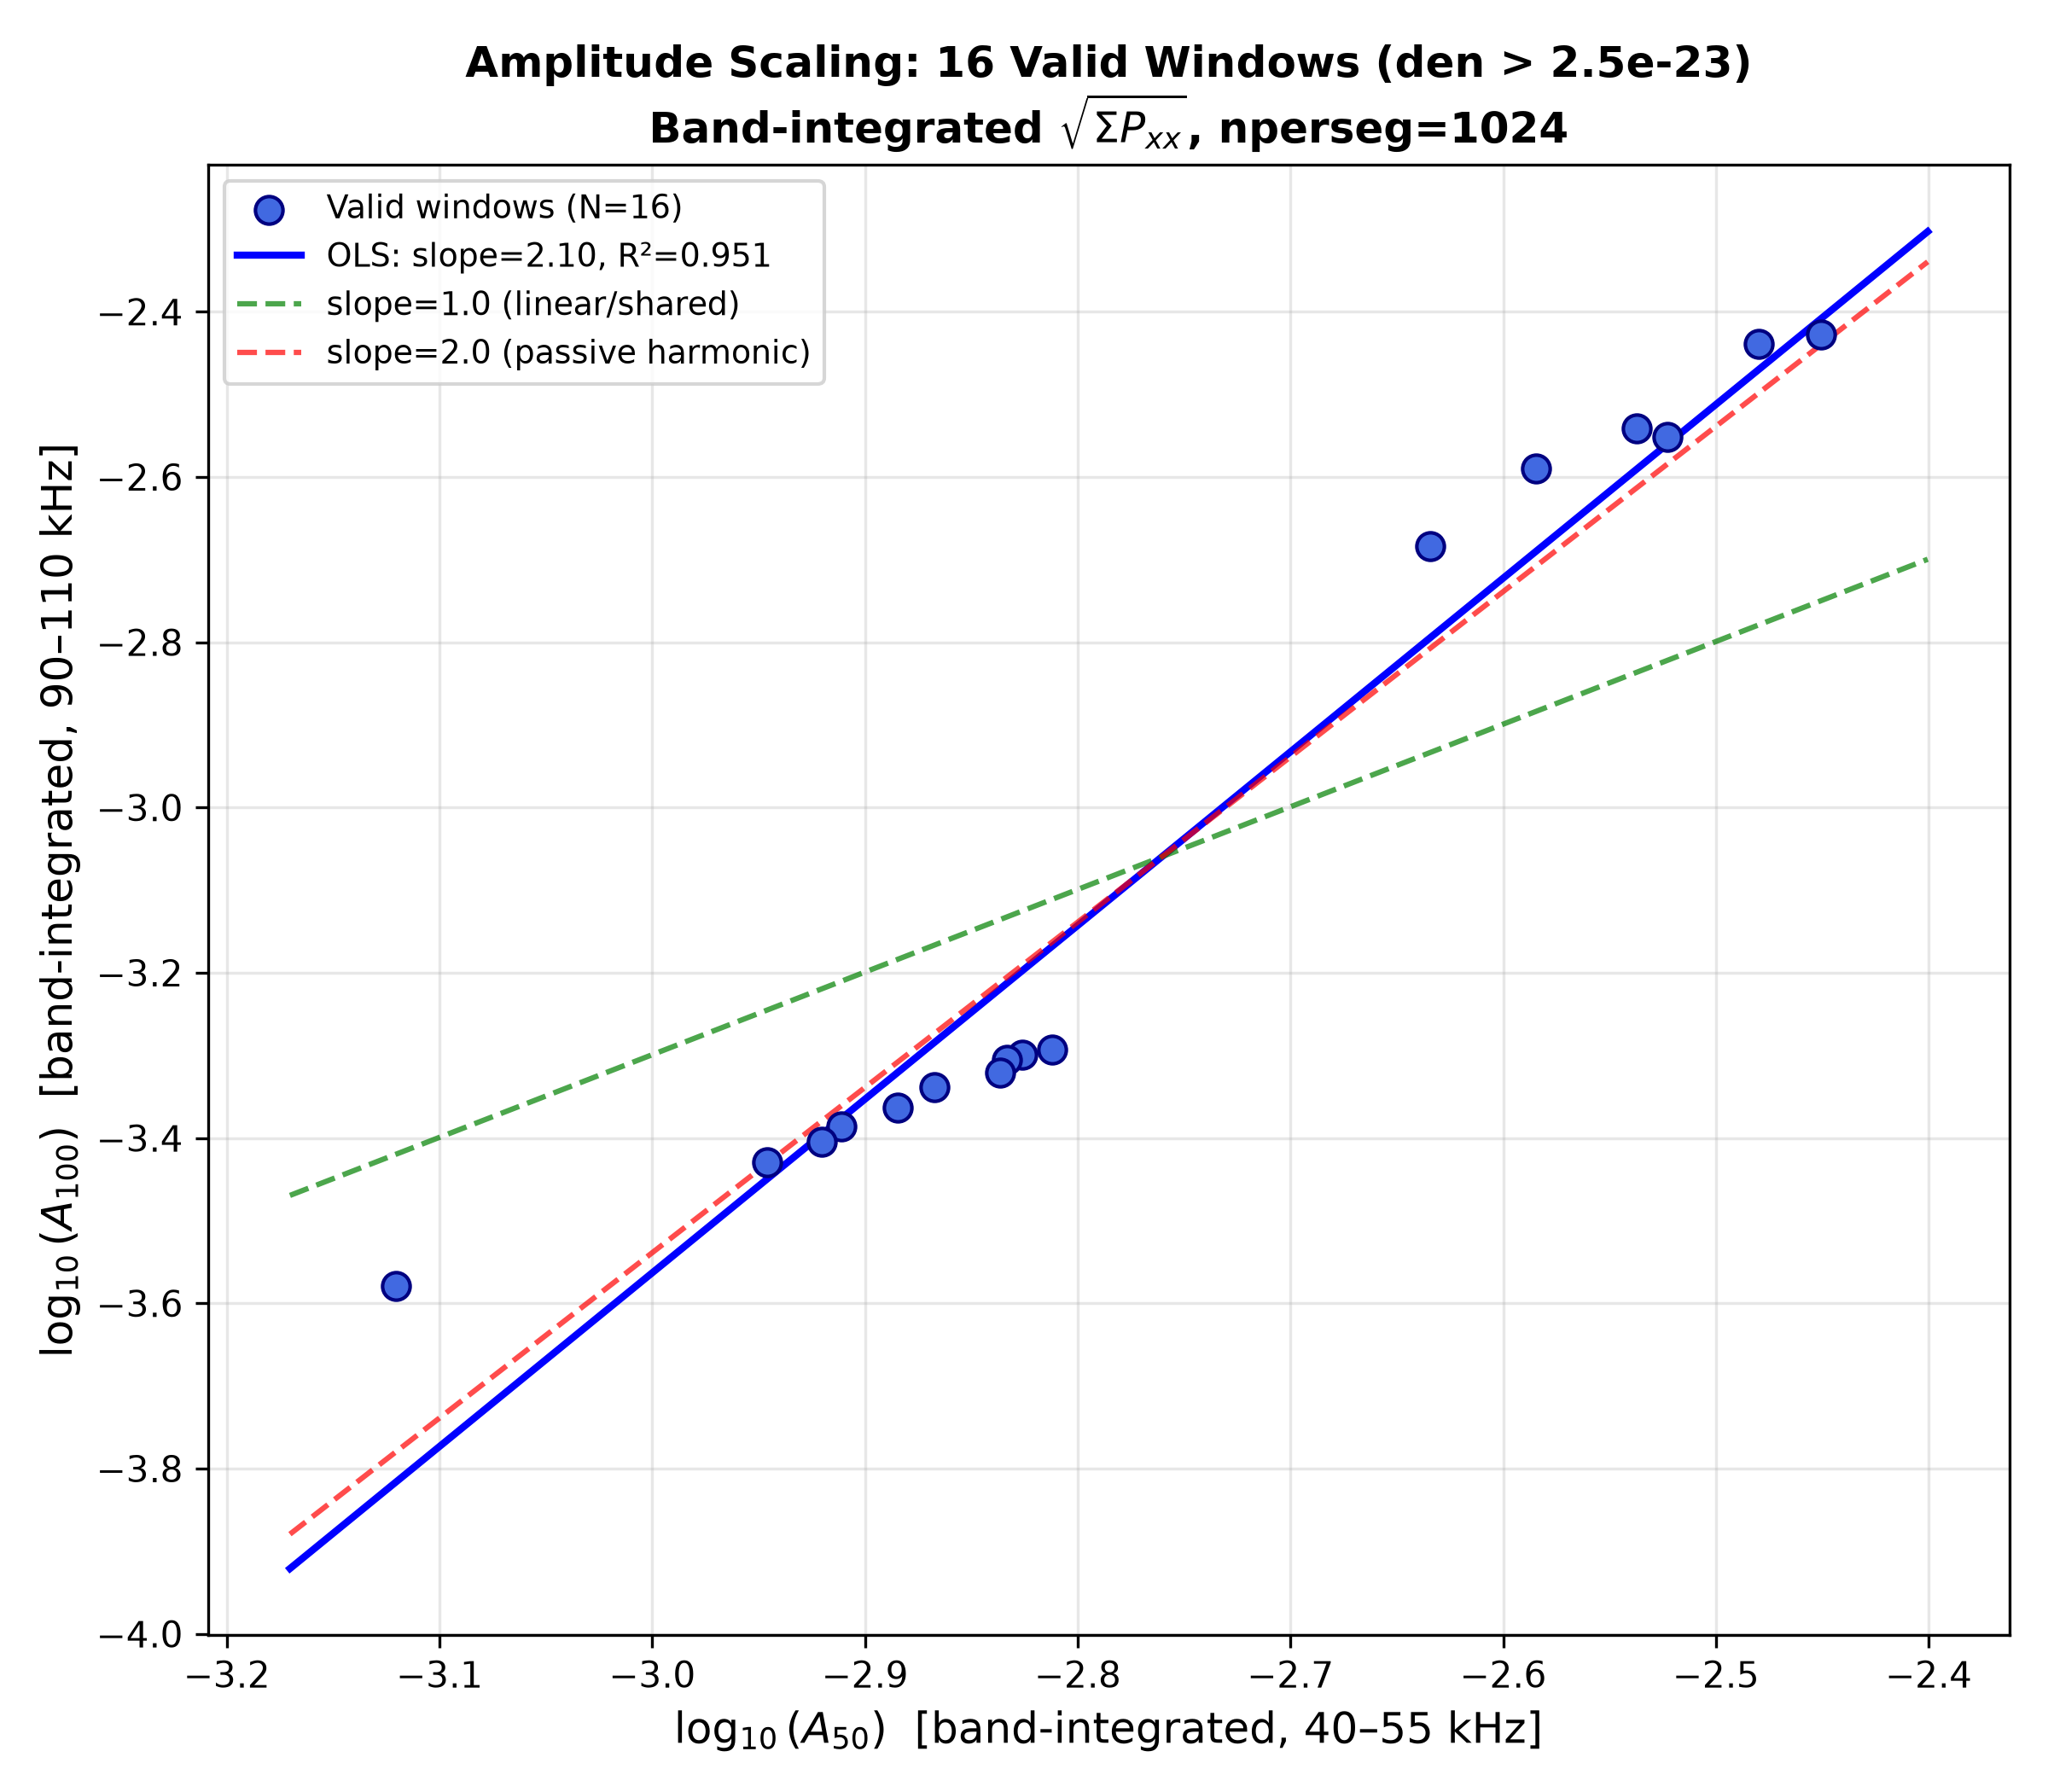
\includegraphics[width=\textwidth]{Images/amplitude_scaling_valid16.png}
            \end{figure}
        \end{column}
        \begin{column}{0.58\textwidth}
            \scriptsize
            \begin{itemize}
                \item Does the lower mode drive a passive harmonic (slope 2), or are they independently driven/shared envelope (slope 1)?
                \item \textbf{Pooled scaling:} $2.10$ (band) to $2.26$ (peak PSD) on the 16 valid windows. Block-bootstrap CI is $[0.94,\;2.37]$.
                \item \textbf{Within-episode:} $1.39$ ($N=6$) and $0.95$ ($N=10$). The pooled $2.10$ value mostly reflects the amplitude drop between episodes ($\sim 2$ effective independent samples).
                \item \textbf{Band peaks:} Lower band peaks at ${\sim}\SI{40}{kHz}$, upper band at $90{-}\SI{105}{kHz}$. The ratio ranges from $2.21{-}2.57$ ($0/16$ windows fall within 5\% of 2.0).
                \item \textbf{Triads:} Only windows 1, 2, and 5 are a clean ${\sim}50+50 \to {\sim}100$\,kHz pair. Episode 2's strongest triads hop ($44.9+66.4 \to 111.3$ and $58.6+70.3 \to 128.9$\,kHz), so the $A_{100}$ vs $A_{50}$ scaling is not a test of a single harmonic interaction.
                \item \textbf{Bottom line:} Scaling is inconclusive; a strict passive second harmonic is disfavored by the frequency ratio.
                \item \textbf{Not stationary:} the strongest triad is the same ($\pm2$ bins) in only 41\% of 8\,ms windows; the most common triad has mean $b^2=0.066$ (noise level) in 8\,ms windows and $0.0004$ over the full burst -- intermittent coupling that moves between triads.
            \end{itemize}
        \end{column}
    \end{columns}
\end{frame}

% SLIDE 13 -- Obj 3 validation status (~80s)
\begin{frame}{Objective 3: Real Coupling, Not Yet a Confirmed Mechanism}
    \footnotesize
    \begin{itemize}
        \item \textbf{What is confirmed:} asymptotic convergence ($1/N\to0$)
        gives a non-zero intercept ($b^2_\infty\approx0.28$--$0.33$ for the
        leading triads vs.\ $\approx0$ for the noise baseline) -- a
        \textbf{real} quadratic phase coupling, not a finite-sample artifact.
        \item \textbf{What fails:} strict double-validation -- shot
        \#88654 reproduces the primary mode (matching coherence,
        $\sim$\SI{2}{kHz} downshift) but not the coupling ($b^2\le0.34$
        vs.\ \num{0.50} required, backup); a scan of 36 Langmuir probe
        tips found \textbf{zero} matches above $b^2>0.5$.
        \item \textbf{Self-critical check:} the burst window is \emph{not}
        statistically superior to quiescent (max $b^2=0.37$) or control
        (max $b^2=0.46$) periods -- no rigorous basis to call this an
        exclusive H-mode signature.
        \item \textbf{Comparative:} NBI-only triads reach up to $\sim$3$\times$
        higher $b^2$ than ECH+NBI (8\,ms sub-windows) -- coupling appears to strengthen once ECH switches off, but the same validation caveat applies.
        \item \textbf{Conclusion:} statistically real; upward in the highest-SNR
        windows (threshold-dependent), but \emph{not yet independently confirmed}
        as a specific mechanism -- reported honestly as an open finding.
    \end{itemize}
\end{frame}

% ============================================================
\section{Conclusions}
% ============================================================

% SLIDE 14 -- Conclusions (~85s)
\begin{frame}{Conclusions}
    \footnotesize
    \begin{itemize}
        \item \textbf{Objective 1:} A single $m=+3$ energetic-particle-like mode at
        $\sim$\SI{89}{kHz} ($n\equiv-1$ mod 4; best fit $n=-5$) is identified in the
        magnetic data and \textbf{keeps its identity}
        across ECH shut-off -- only its frequency shifts. ECE fluctuation in the mode band
        peaks near $\rho\approx0.62$ but is not coherent with MP1, so radial localization
        is suggestive only.
        \item \textbf{Objective 2:} The mode envelope correlates strongly with heating and
        confinement metrics ($r=0.57$--$0.87$ for $I_p$, $W_p$, $n_e$, H$\alpha$ in both
        bands; consistent with \textbf{NBI drive} rather than ECH), establishing the
        EPM--heating link. The Primary poloidal structure is \textbf{confirmed} ($m=+3$; Secondary
        unconfirmed); band-separated scaling-model tests are inconclusive -- no model is
        statistically significant.
        \item \textbf{Objective 3:} Three-wave phase coupling is \textbf{statistically real}; early at $f/2$, later shifting to asymmetric triads that hop between windows. Energy flows \textbf{upward} in the 16 highest-SNR windows (${\sim}2$ independent episodes; the sign is threshold-dependent). Not validated under the strict double criterion; mode identity and mechanism remain \textbf{open questions}.
        \item \textbf{Confinement relevance:} the primary mode's edge/core
        localization and weak edge-H$\alpha$ coupling ($\gamma^2=0.23$) make it a
        possible fast-ion/heat-loss channel, though a direct transport
        coefficient has not yet been quantified -- a natural next step.
    \end{itemize}
    \vspace{0.2cm}
    \textbf{Next steps:} re-analysis with a working validation shot, a
    refined Langmuir cross-check, phase-locking tests to resolve mode
    identity, and extension of this pipeline to a broader shot database.
\end{frame}

% SLIDE 14b -- Thesis objectives status summary
\begin{frame}{Thesis Objectives: Status Summary}
    \footnotesize
    \begin{center}
    \renewcommand{\arraystretch}{1.3}
    \begin{tabular}{p{6.4cm}p{5.7cm}c}
        \toprule
        Specific objective (thesis \S1.3.2) & Delivered evidence & Status \\
        \midrule
        Spectral properties \& temporal evolution; dominant modes &
        $m={+}3$ mode at $\sim$\SI{89}{kHz}, $n\equiv{-}1$; survives ECH shut-off &
        \textbf{Met} \\
        EPM--heating correlation; statistical metrics &
        $r=0.57$--$0.87$ vs.\ $I_p$, $W_p$, $n_e$, H$\alpha$; NBI drive $>$ ECH &
        \textbf{Met} \\
        Secondary-band H-mode fluctuations; edge turbulence \& heat-transport coupling &
        Bicoherence real \& unidirectional; edge/H$\alpha$ coupling weak
        ($\gamma^2=0.23$); double-validation not passed &
        \textbf{Partial} \\
        \bottomrule
    \end{tabular}
    \end{center}
    \vspace{0.3cm}
    \normalsize
    The third objective is the one where the evidence is weakest: the
    non-linear coupling is statistically real and consistently unidirectional,
    but its specific tie to edge turbulence / enhanced heat transport is not yet
    independently confirmed -- reported honestly as open, not overstated.
\end{frame}

% SLIDE 15 -- Thank you / Questions
\begin{frame}
    \begin{center}
        {\Huge Thank you}\\[0.5cm]
        {\Large Questions?}
    \end{center}
\end{frame}

% ================================================================
% ================================================================
%                        BACKUP SLIDES
% ================================================================
% ================================================================
\appendix
\section{Backup Slides}

\begin{frame}
    \begin{center}
        {\usebeamerfont{title}\structure{\Huge Backup Slides}}
    \end{center}
\end{frame}

\subsection{Backup: Objective 1}



\begin{frame}{Backup: Objective 1 -- Radial Fluctuation Profile}
    \begin{figure}[h!]
        \centering
        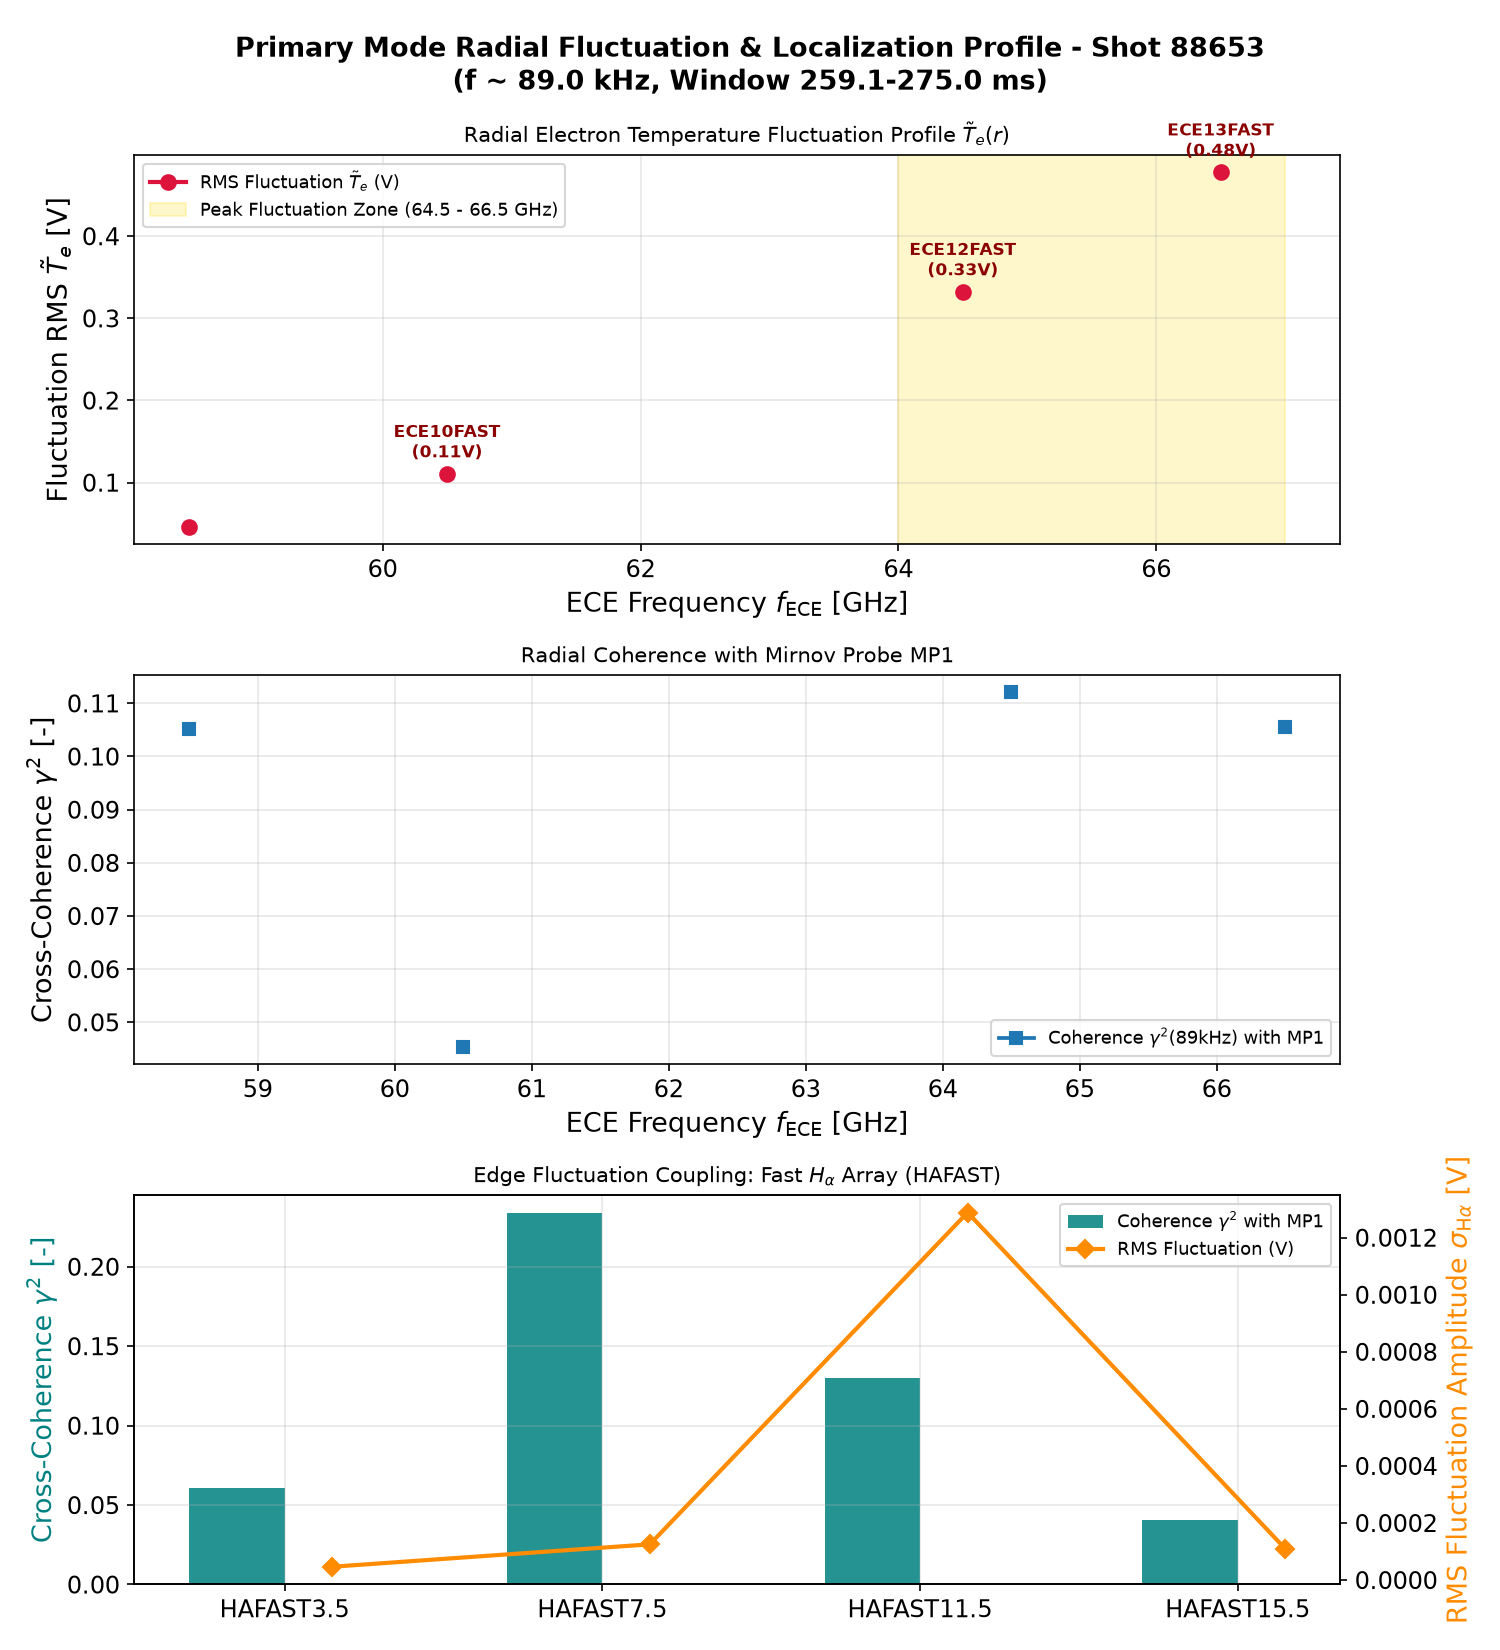
\includegraphics[height=0.74\textheight]{Images/obj1_mode_identification/mhd_primary_mode_radial_profile_shot_88653.png}
    \end{figure}
    \vspace{-0.3cm}
    {\tiny RMS of the \SIrange{80}{100}{kHz} band, \SIrange{259.1}{275.0}{ms}. Omitted: ECE1--7, 11, 14 (active = quiet RMS: dead or outside the plasma) and ECE8, 15, 16 ($<0.01$\,V). ECE12--13 are mutually coherent (0.77 at \SI{89}{kHz}); ECE--MP1 coherence (0.05--0.11) is below its floor (0.20).}
\end{frame}

\begin{frame}{Backup: Objective 1 Comparative -- Zoomed Spectrograms}
    \begin{columns}[T]
        \begin{column}{0.5\textwidth}
            \centering ECH+NBI (259.1--291.3 ms)\\
            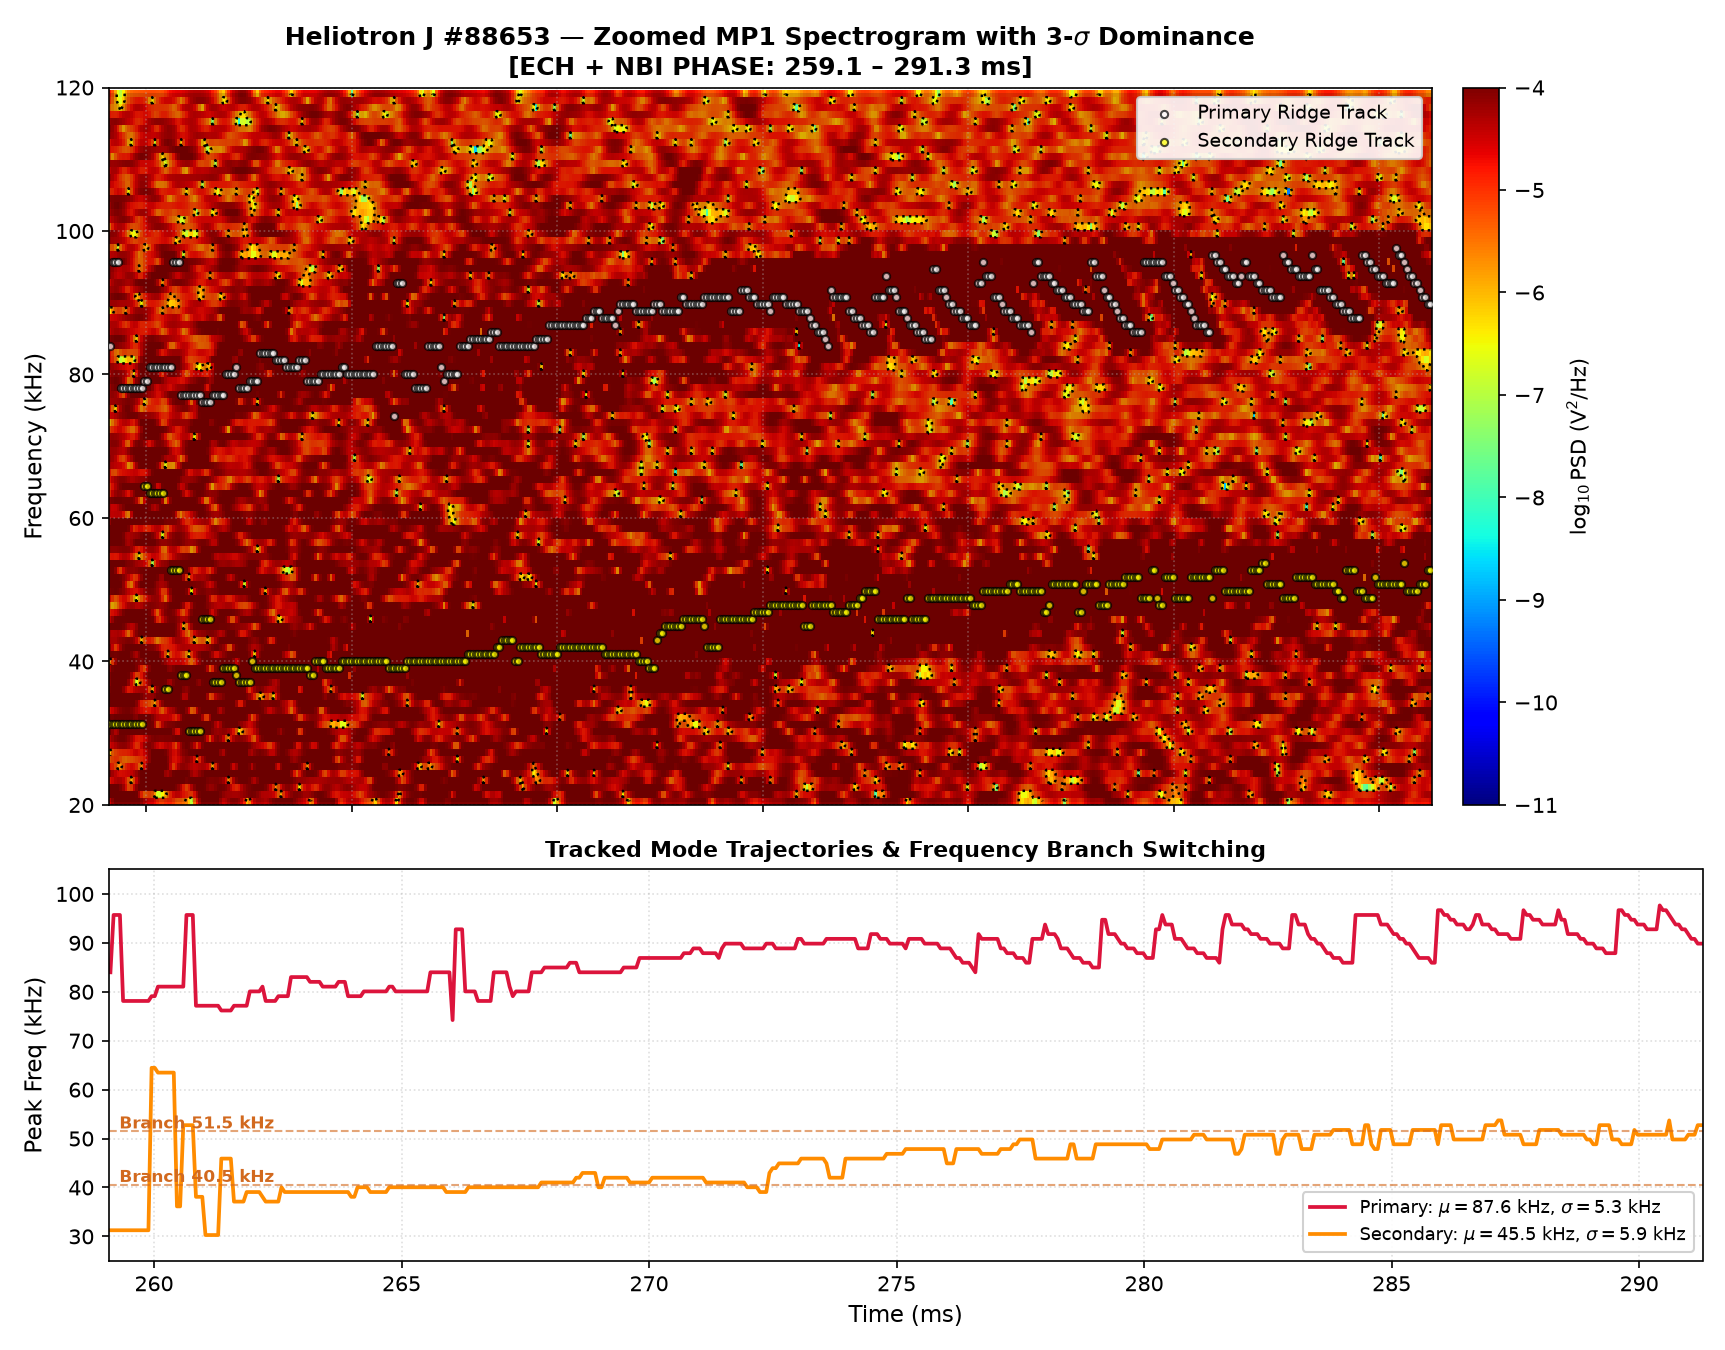
\includegraphics[width=\textwidth]{Images/heating_phase_comparison/zoomed_spectrogram_3sigma_ECH_NBI_259.1_291.3ms.png}
        \end{column}
        \begin{column}{0.5\textwidth}
            \centering NBI-only (291.3--300.0 ms)\\
            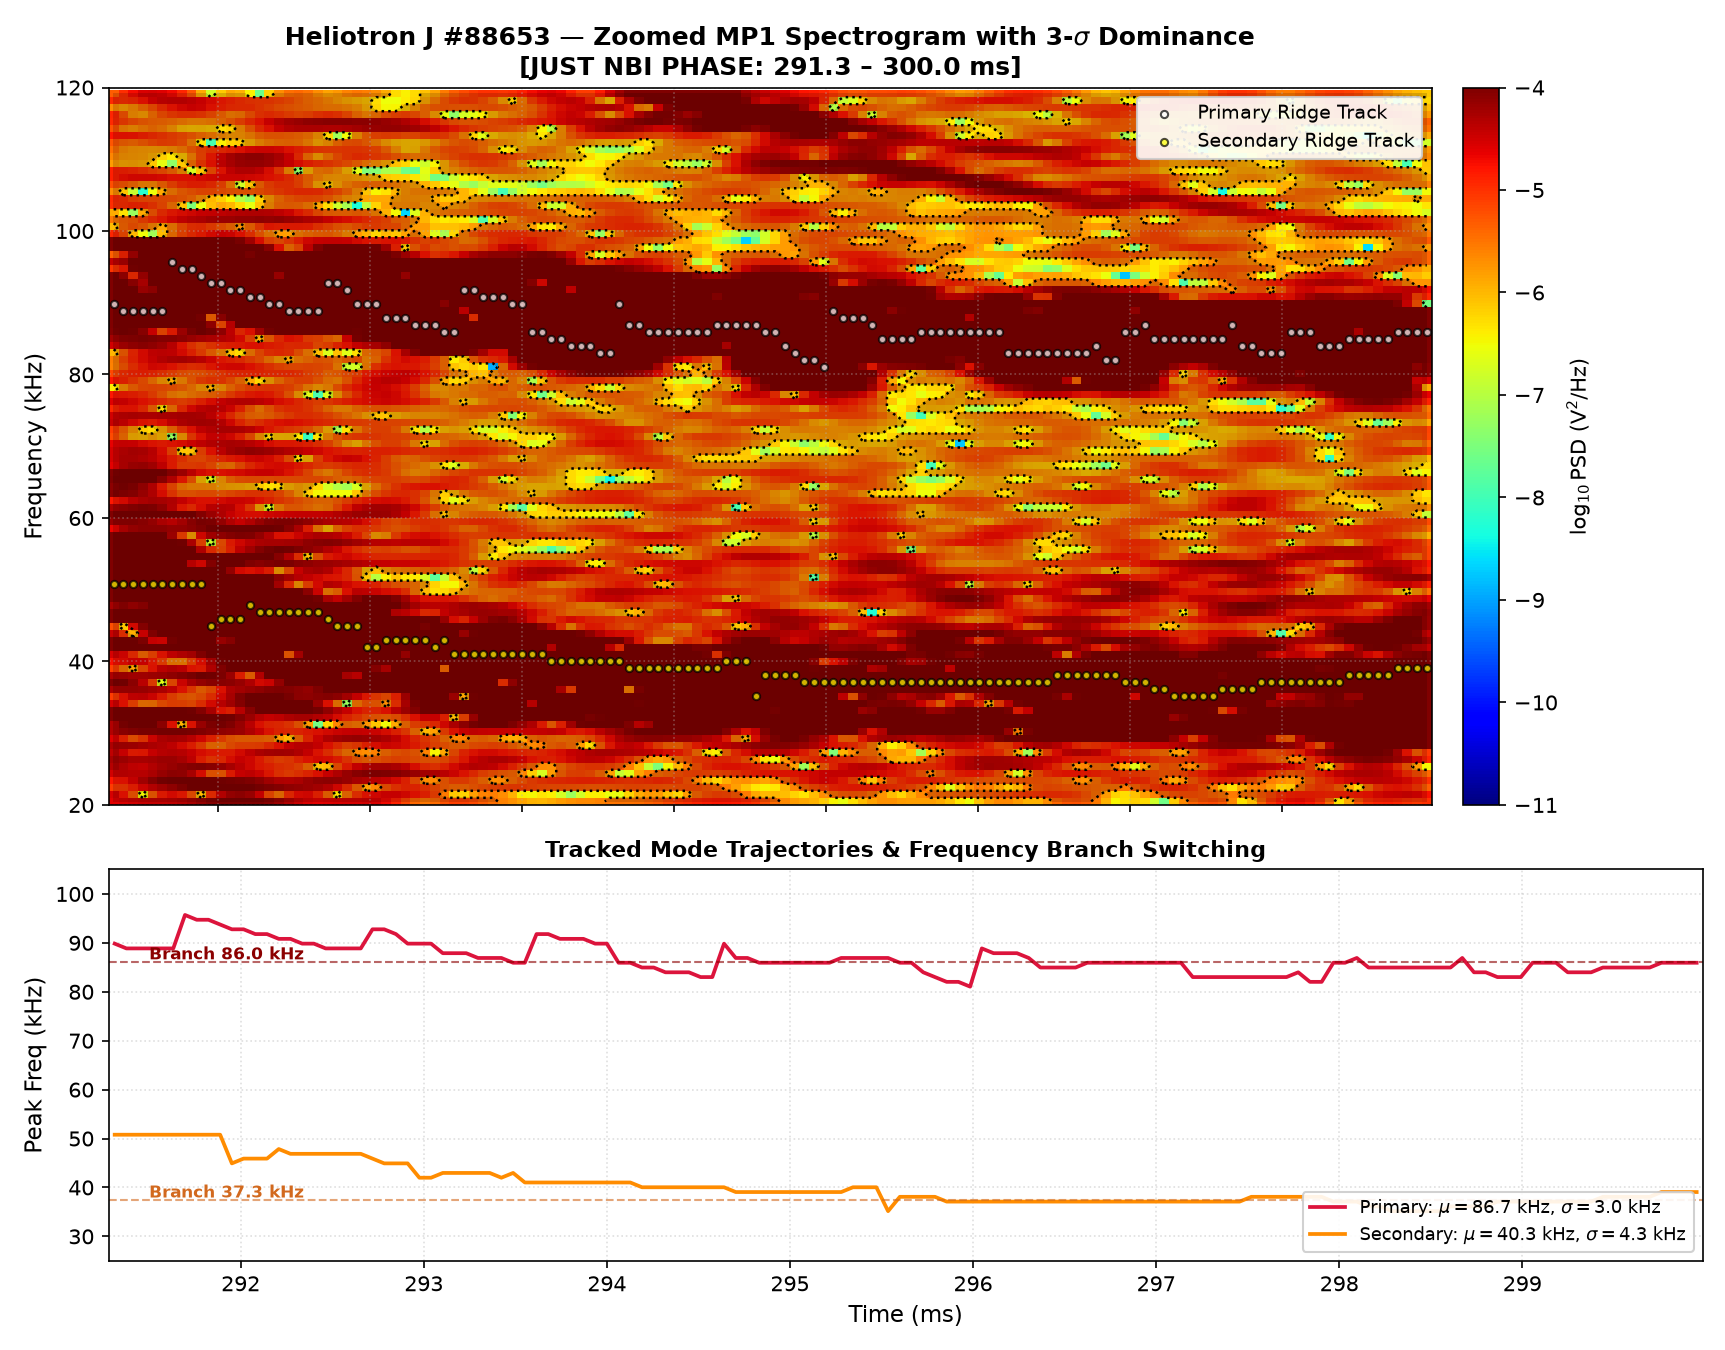
\includegraphics[width=\textwidth]{Images/heating_phase_comparison/zoomed_spectrogram_3sigma_NBI_only_291.3_300.0ms.png}
        \end{column}
    \end{columns}
\end{frame}

\begin{frame}{Backup: Objective 1 Comparative -- Mode Identification Overview}
    \begin{columns}[T]
        \begin{column}{0.4\textwidth}
            \centering ECH+NBI\\
            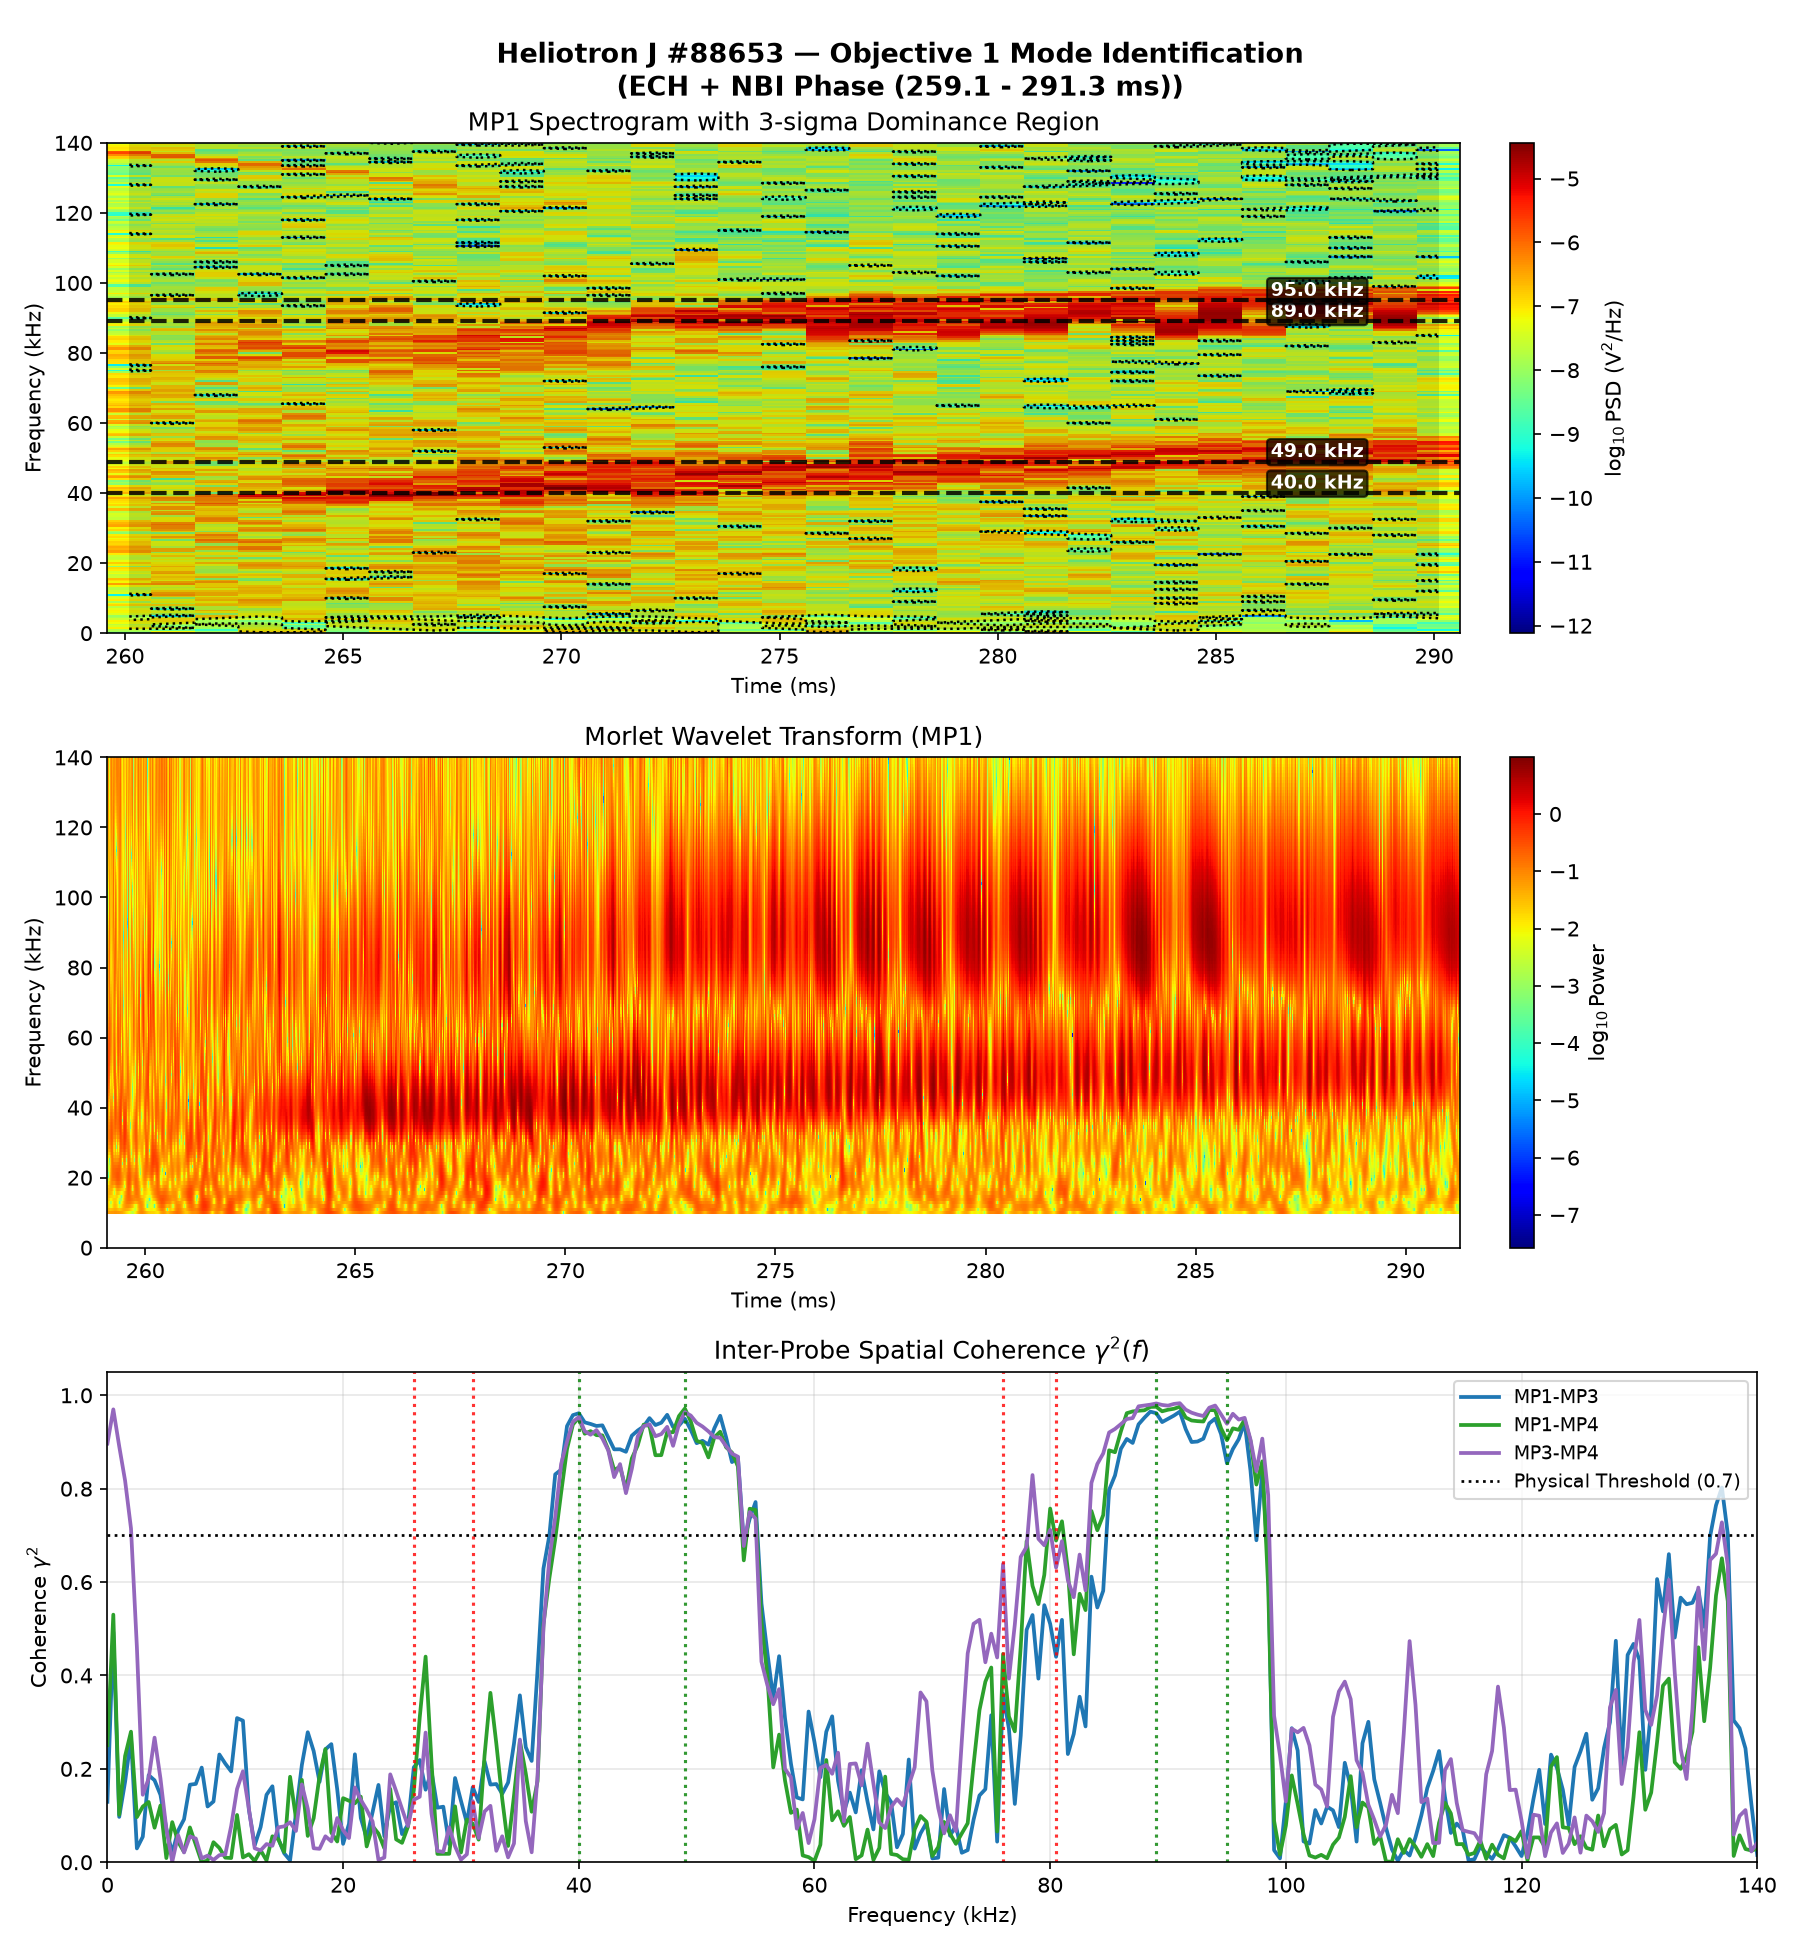
\includegraphics[width=\textwidth]{Images/heating_phase_comparison/mhd_analysis_objective1_88653_ECH_NBI.png}
        \end{column}
        \begin{column}{0.4\textwidth}
            \centering NBI-only\\
            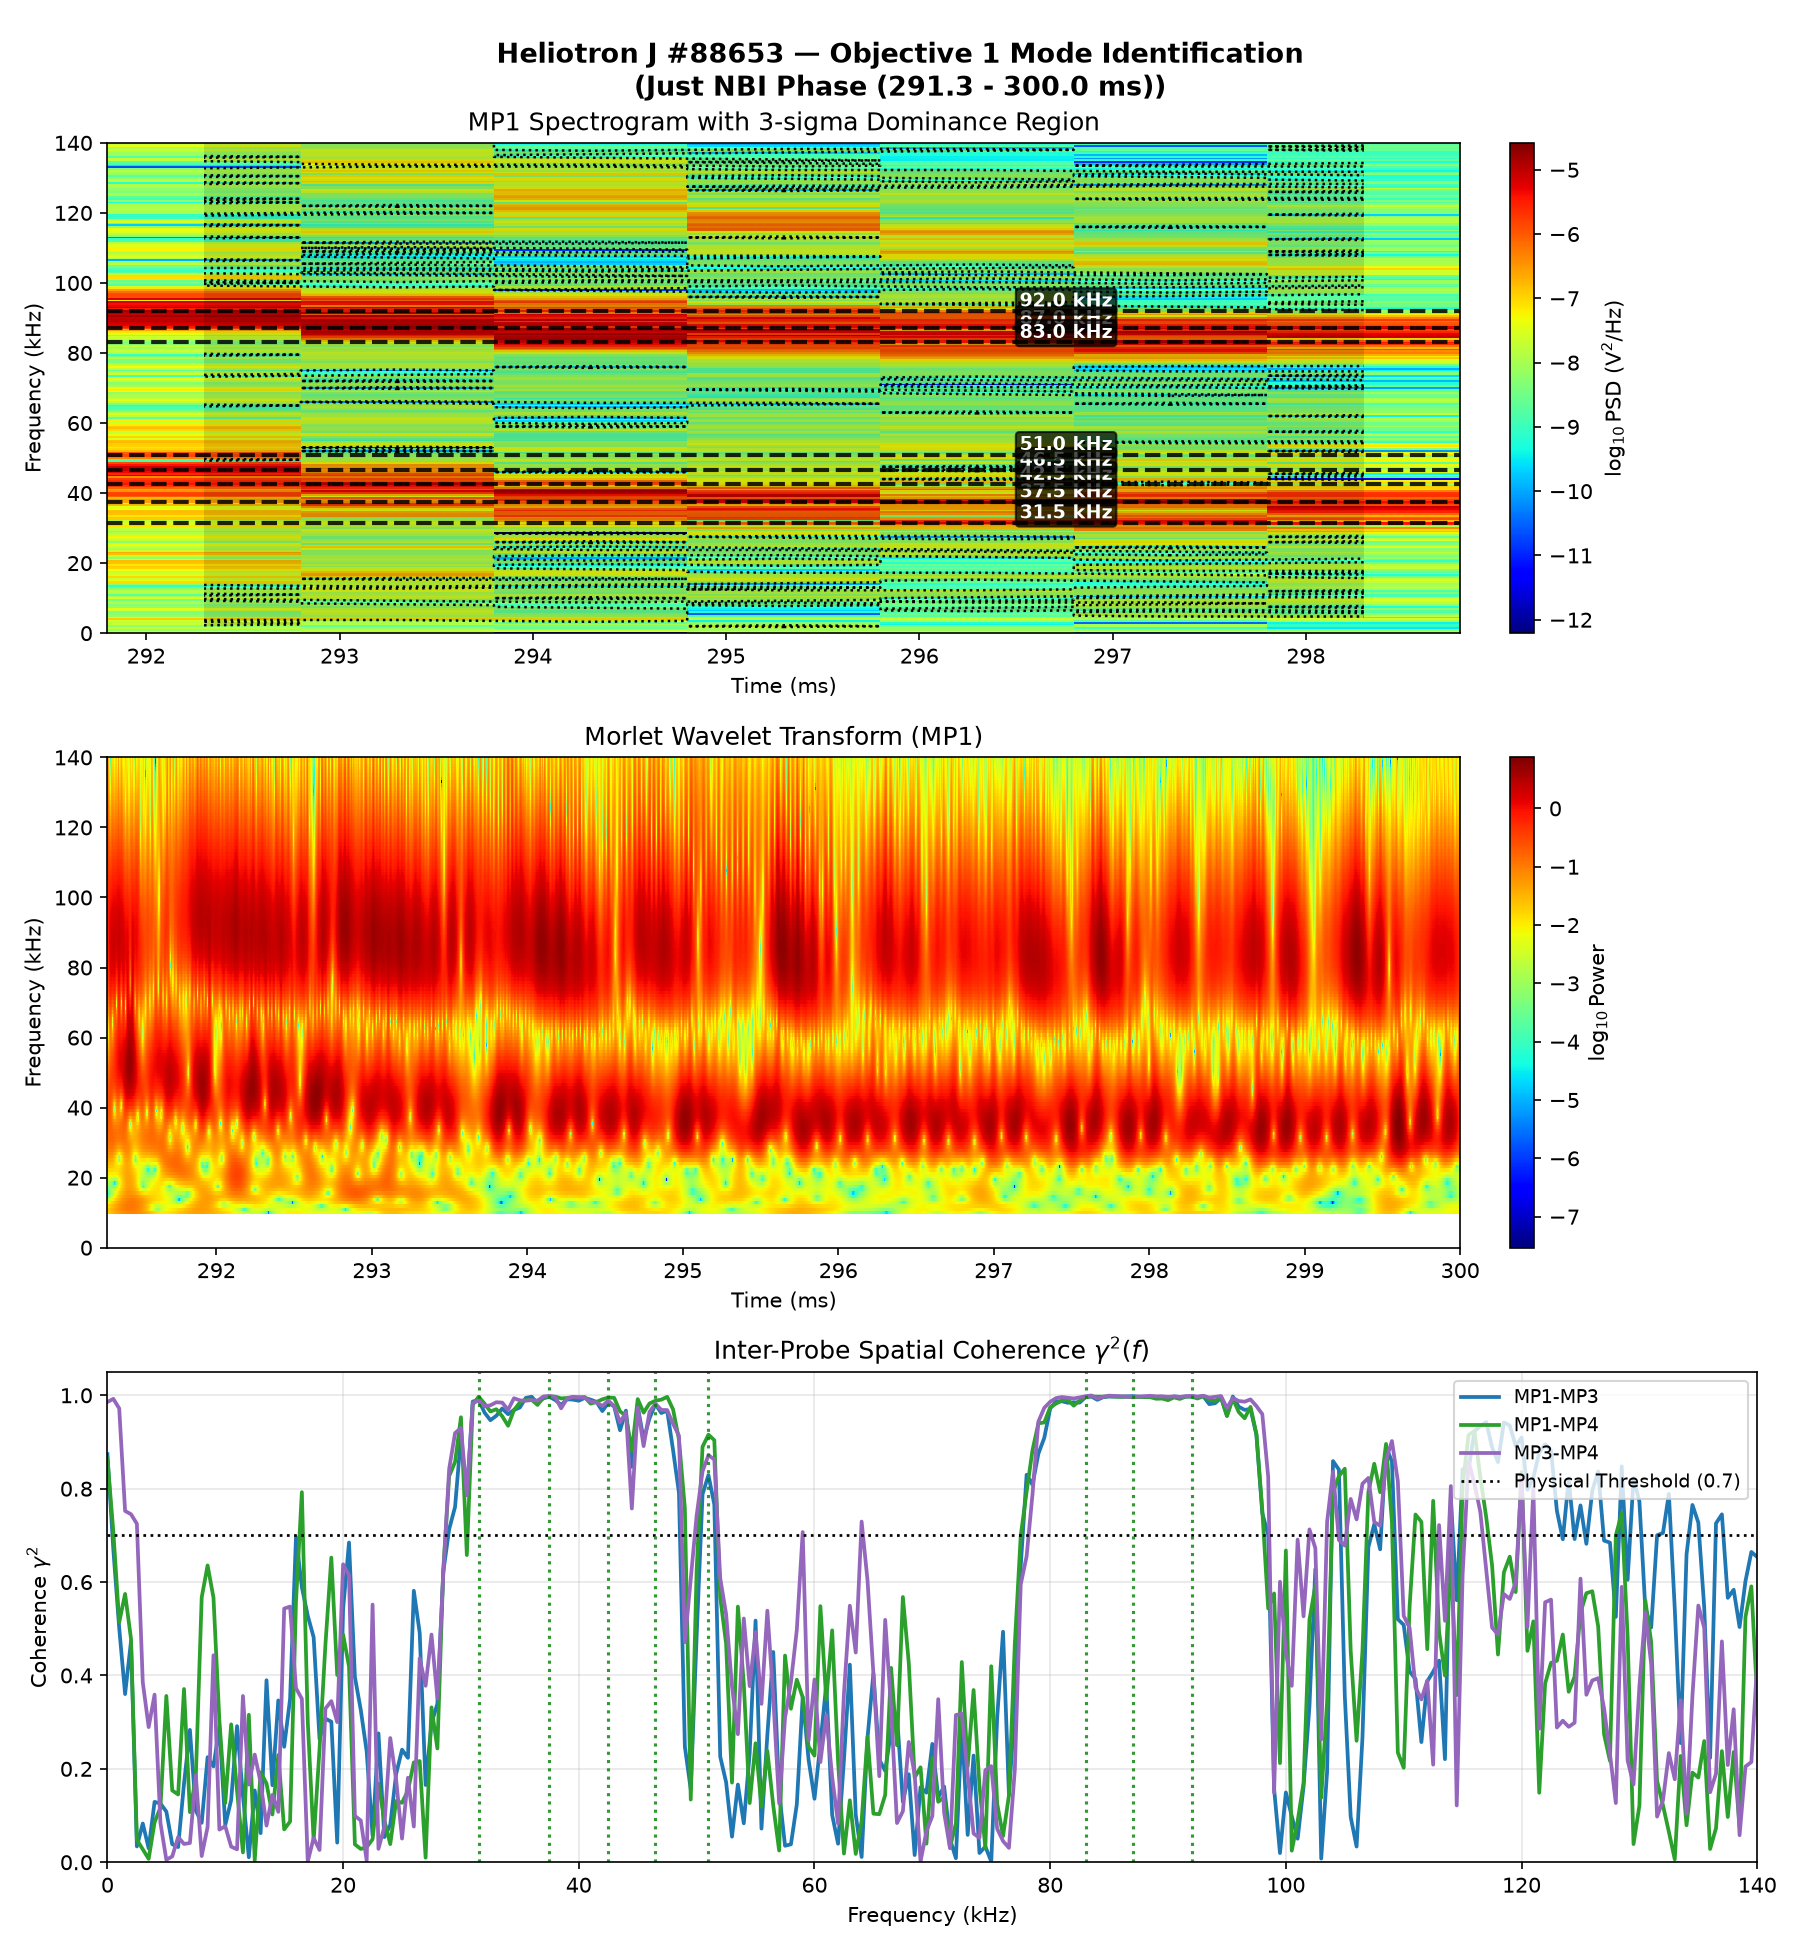
\includegraphics[width=\textwidth]{Images/heating_phase_comparison/mhd_analysis_objective1_88653_NBI_only.png}
        \end{column}
    \end{columns}
\end{frame}

\begin{frame}{Backup: Objective 1 Comparative -- Confirmed Discrete Modes}
    \tiny
    \setlength{\tabcolsep}{5pt}
    \begin{columns}[T]
        \begin{column}{0.48\textwidth}
            \centering \normalsize\textbf{ECH+NBI}\tiny
            \begin{tabular}{cc@{\hspace{6pt}}ccc}
                \toprule
                $f$ (kHz) & Amp. (a.u.) & $\gamma^2_{13}$ & $\gamma^2_{14}$ & $\gamma^2_{34}$ \\
                \midrule
                89.0 & \num{5.36e-6} & 0.962 & 0.975 & 0.983 \\
                49.0 & \num{3.05e-6} & 0.950 & 0.972 & 0.964 \\
                40.0 & \num{2.89e-6} & 0.962 & 0.952 & 0.953 \\
                95.0 & \num{1.78e-6} & 0.854 & 0.904 & 0.939 \\
                \bottomrule
            \end{tabular}
            \vspace{0.15cm}
            \raggedright 4 additional candidates (80.5, 26.0, 76.0, 31.0 kHz) were above the noise floor but failed the coherence criterion.
        \end{column}
        \begin{column}{0.48\textwidth}
            \centering \normalsize\textbf{NBI-only}\tiny
            \begin{tabular}{cc@{\hspace{6pt}}ccc}
                \toprule
                $f$ (kHz) & Amp. (a.u.) & $\gamma^2_{13}$ & $\gamma^2_{14}$ & $\gamma^2_{34}$ \\
                \midrule
                37.5 & \num{8.24e-6} & 0.997 & 0.997 & 0.999 \\
                87.0 & \num{6.76e-6} & 0.998 & 0.996 & 0.997 \\
                83.0 & \num{3.90e-6} & 0.996 & 0.996 & 0.998 \\
                92.0 & \num{3.43e-6} & 0.998 & 0.997 & 0.999 \\
                42.5 & \num{2.41e-6} & 0.984 & 0.995 & 0.989 \\
                31.5 & \num{1.85e-6} & 0.990 & 0.997 & 0.989 \\
                46.5 & \num{1.21e-6} & 0.981 & 0.988 & 0.982 \\
                51.0 & \num{2.17e-7} & 0.829 & 0.916 & 0.872 \\
                \bottomrule
            \end{tabular}
        \end{column}
    \end{columns}
    \vspace{0.2cm}
    \normalsize
    \textbf{Observation:} every candidate mode passes the dual criterion once ECH switches off, and coherence pairs are systematically higher -- consistent with a cleaner, more coherent fluctuation spectrum in the NBI-only phase.
\end{frame}

\subsection{Backup: Objective 2}

\begin{frame}{Backup: Objective 2 -- Secondary Band Macroscopic Correlations}
    \begin{figure}[h!]
        \centering
        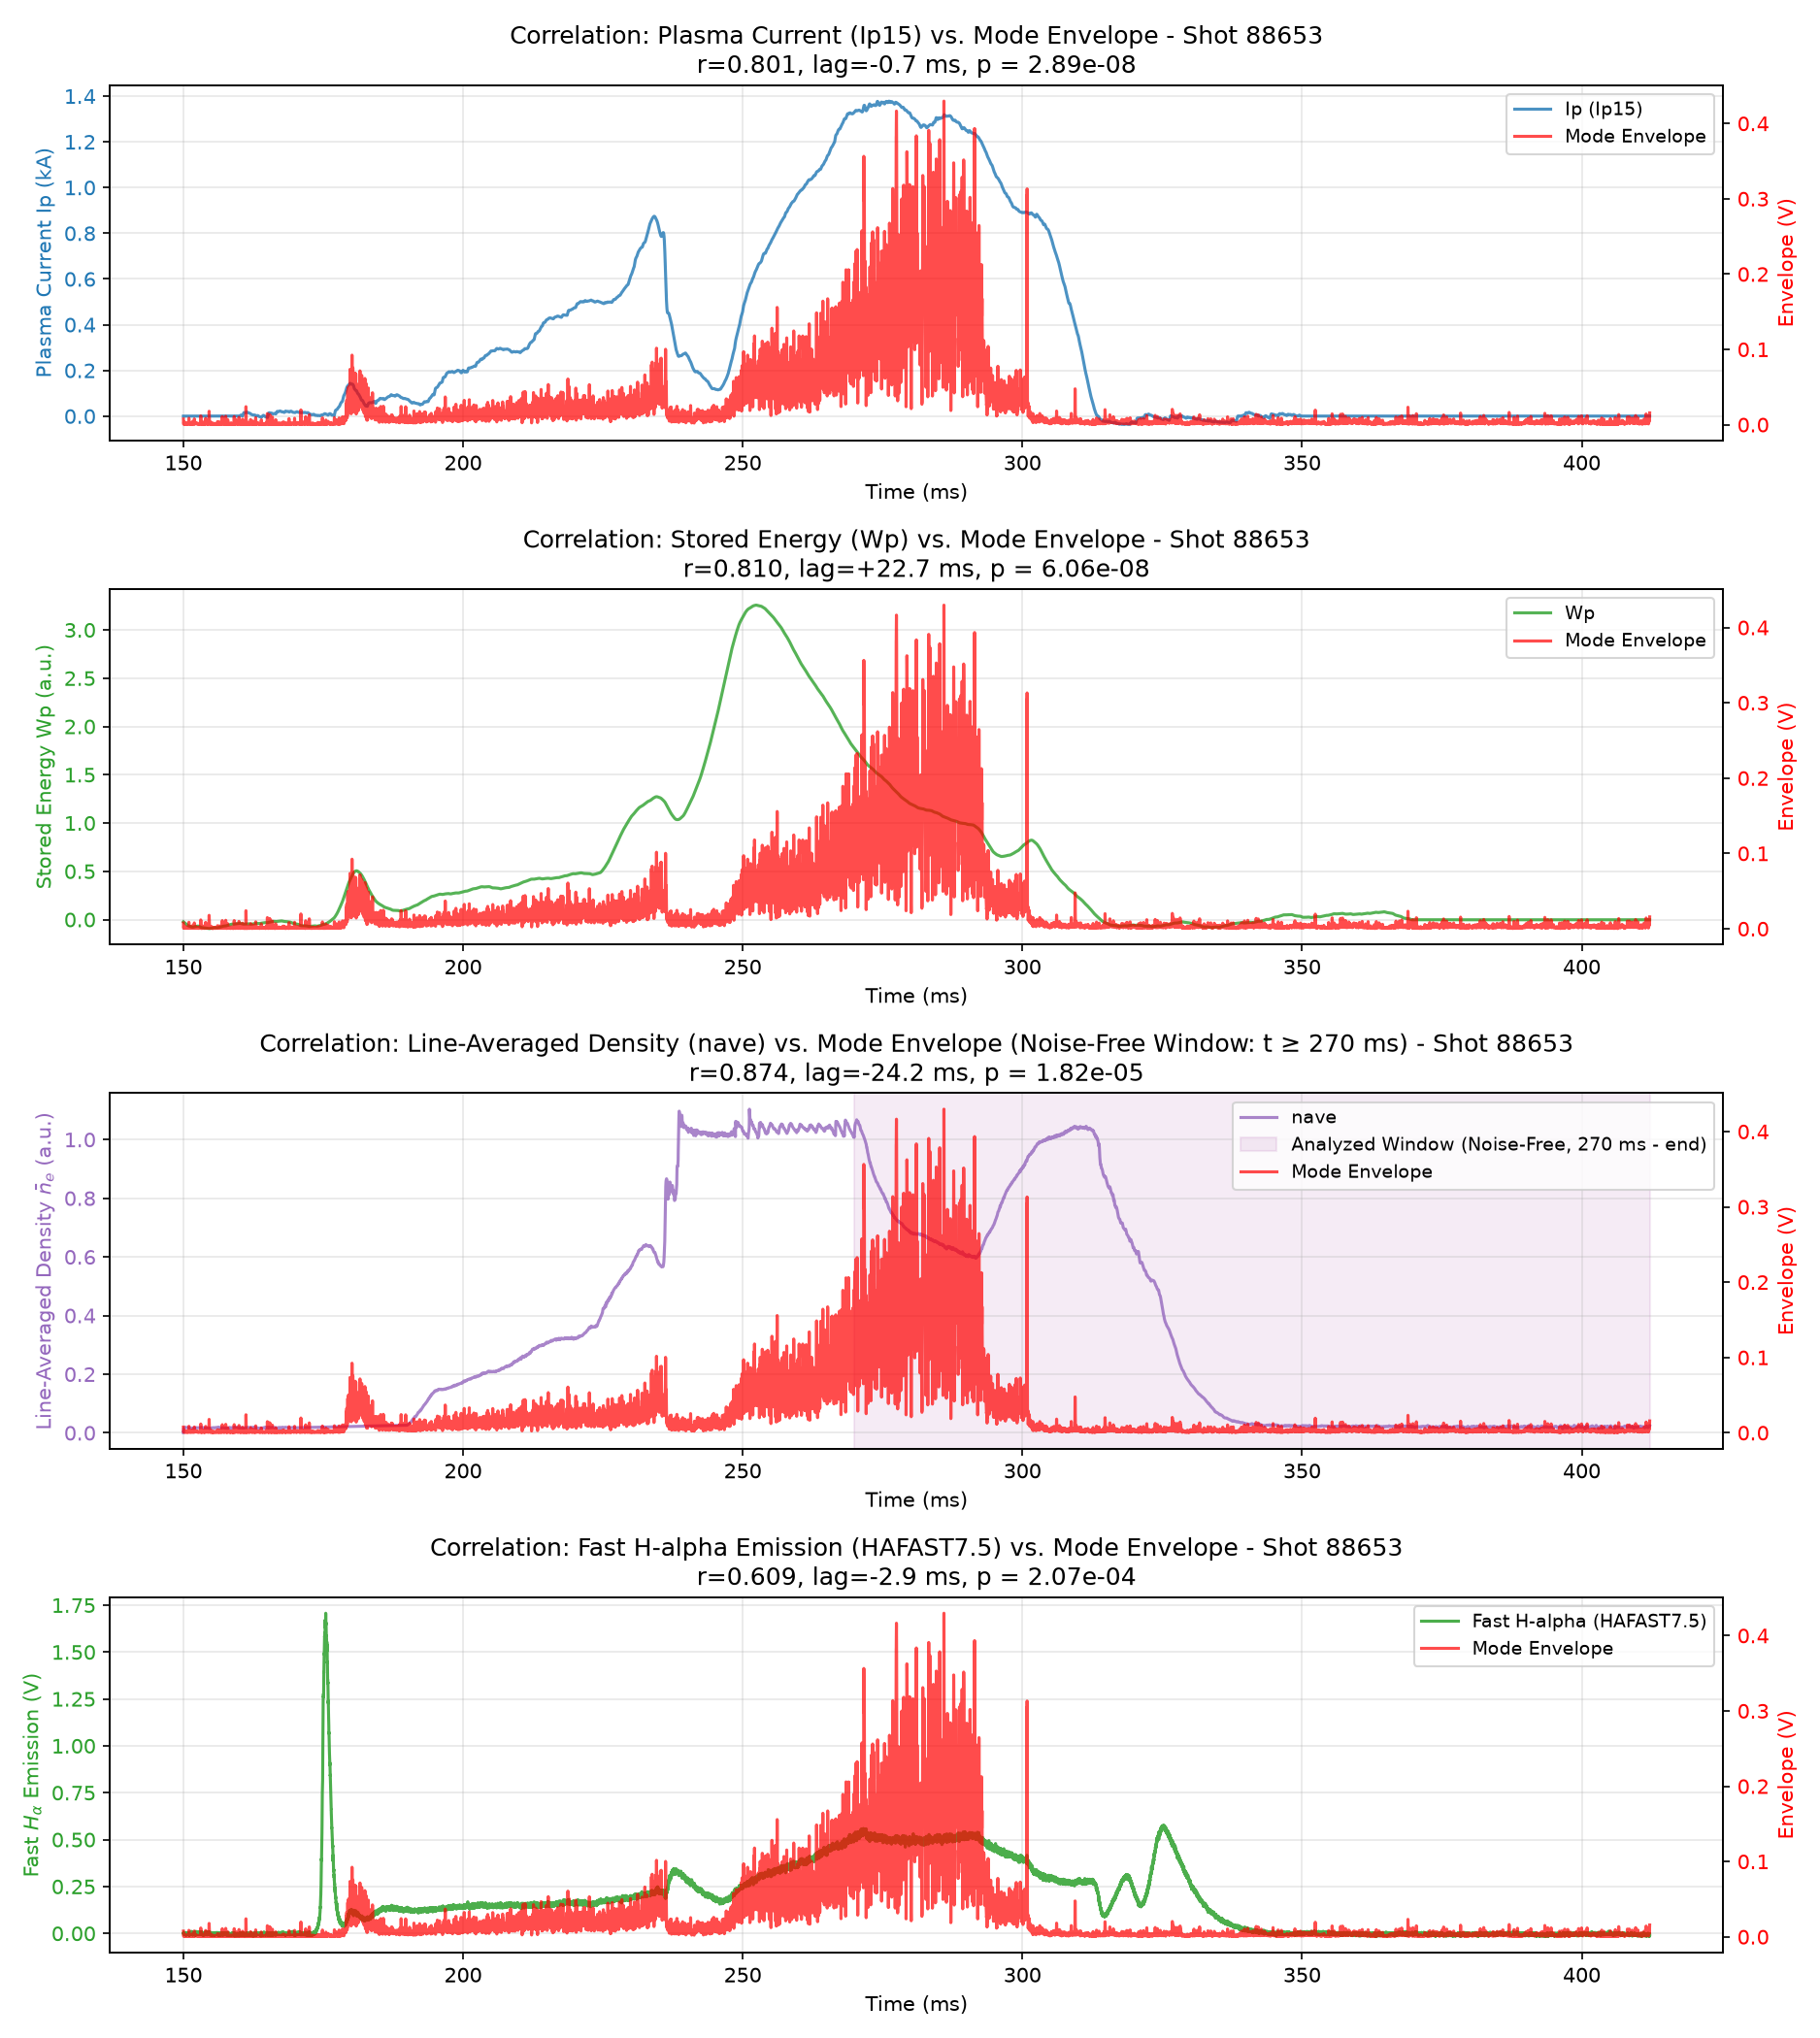
\includegraphics[height=0.85\textheight]{Images/obj2_dynamics_and_structure/mhd_analysis_objective2_88653_40_80kHz.png}
    \end{figure}
\end{frame}

\begin{frame}{Backup: Objective 2 -- Secondary Band Heating Synchronization}
    \begin{figure}[h!]
        \centering
        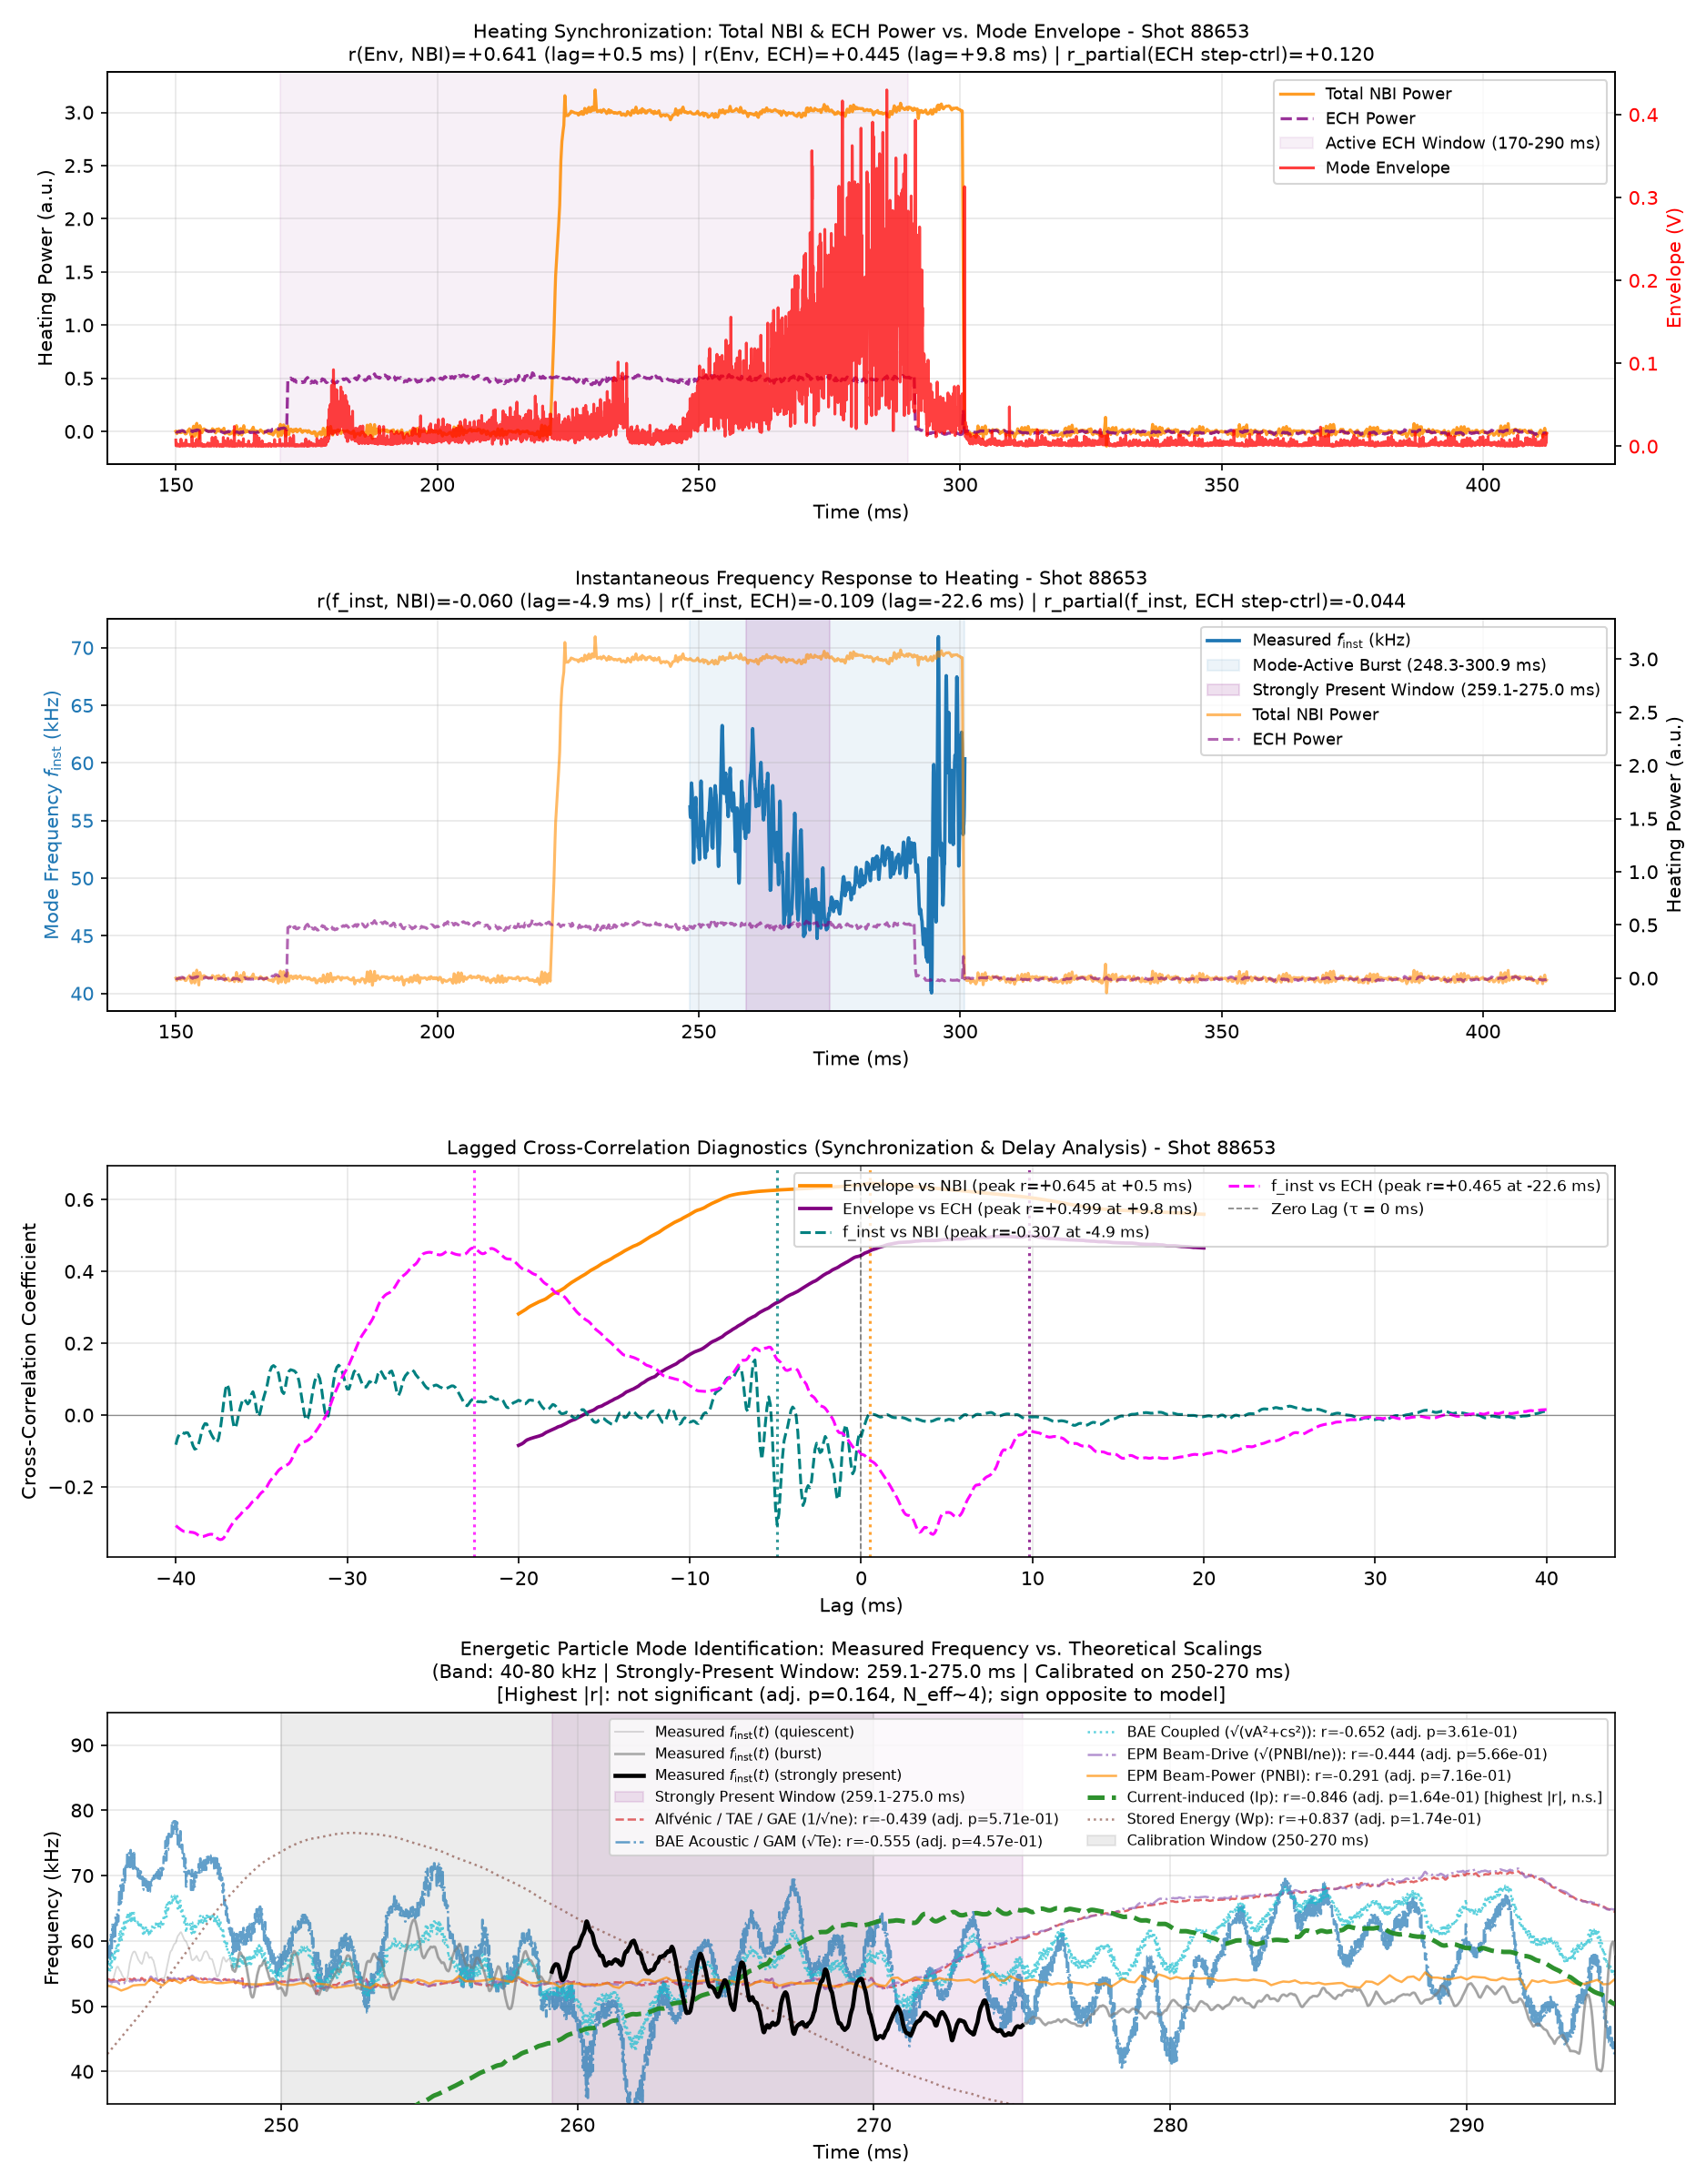
\includegraphics[height=0.85\textheight]{Images/obj2_dynamics_and_structure/mhd_analysis_objective2_heating_88653_40_80kHz.png}
    \end{figure}
\end{frame}

\begin{frame}{Backup: Objective 2 -- Primary Band Macroscopic Correlations}
    \begin{figure}[h!]
        \centering
        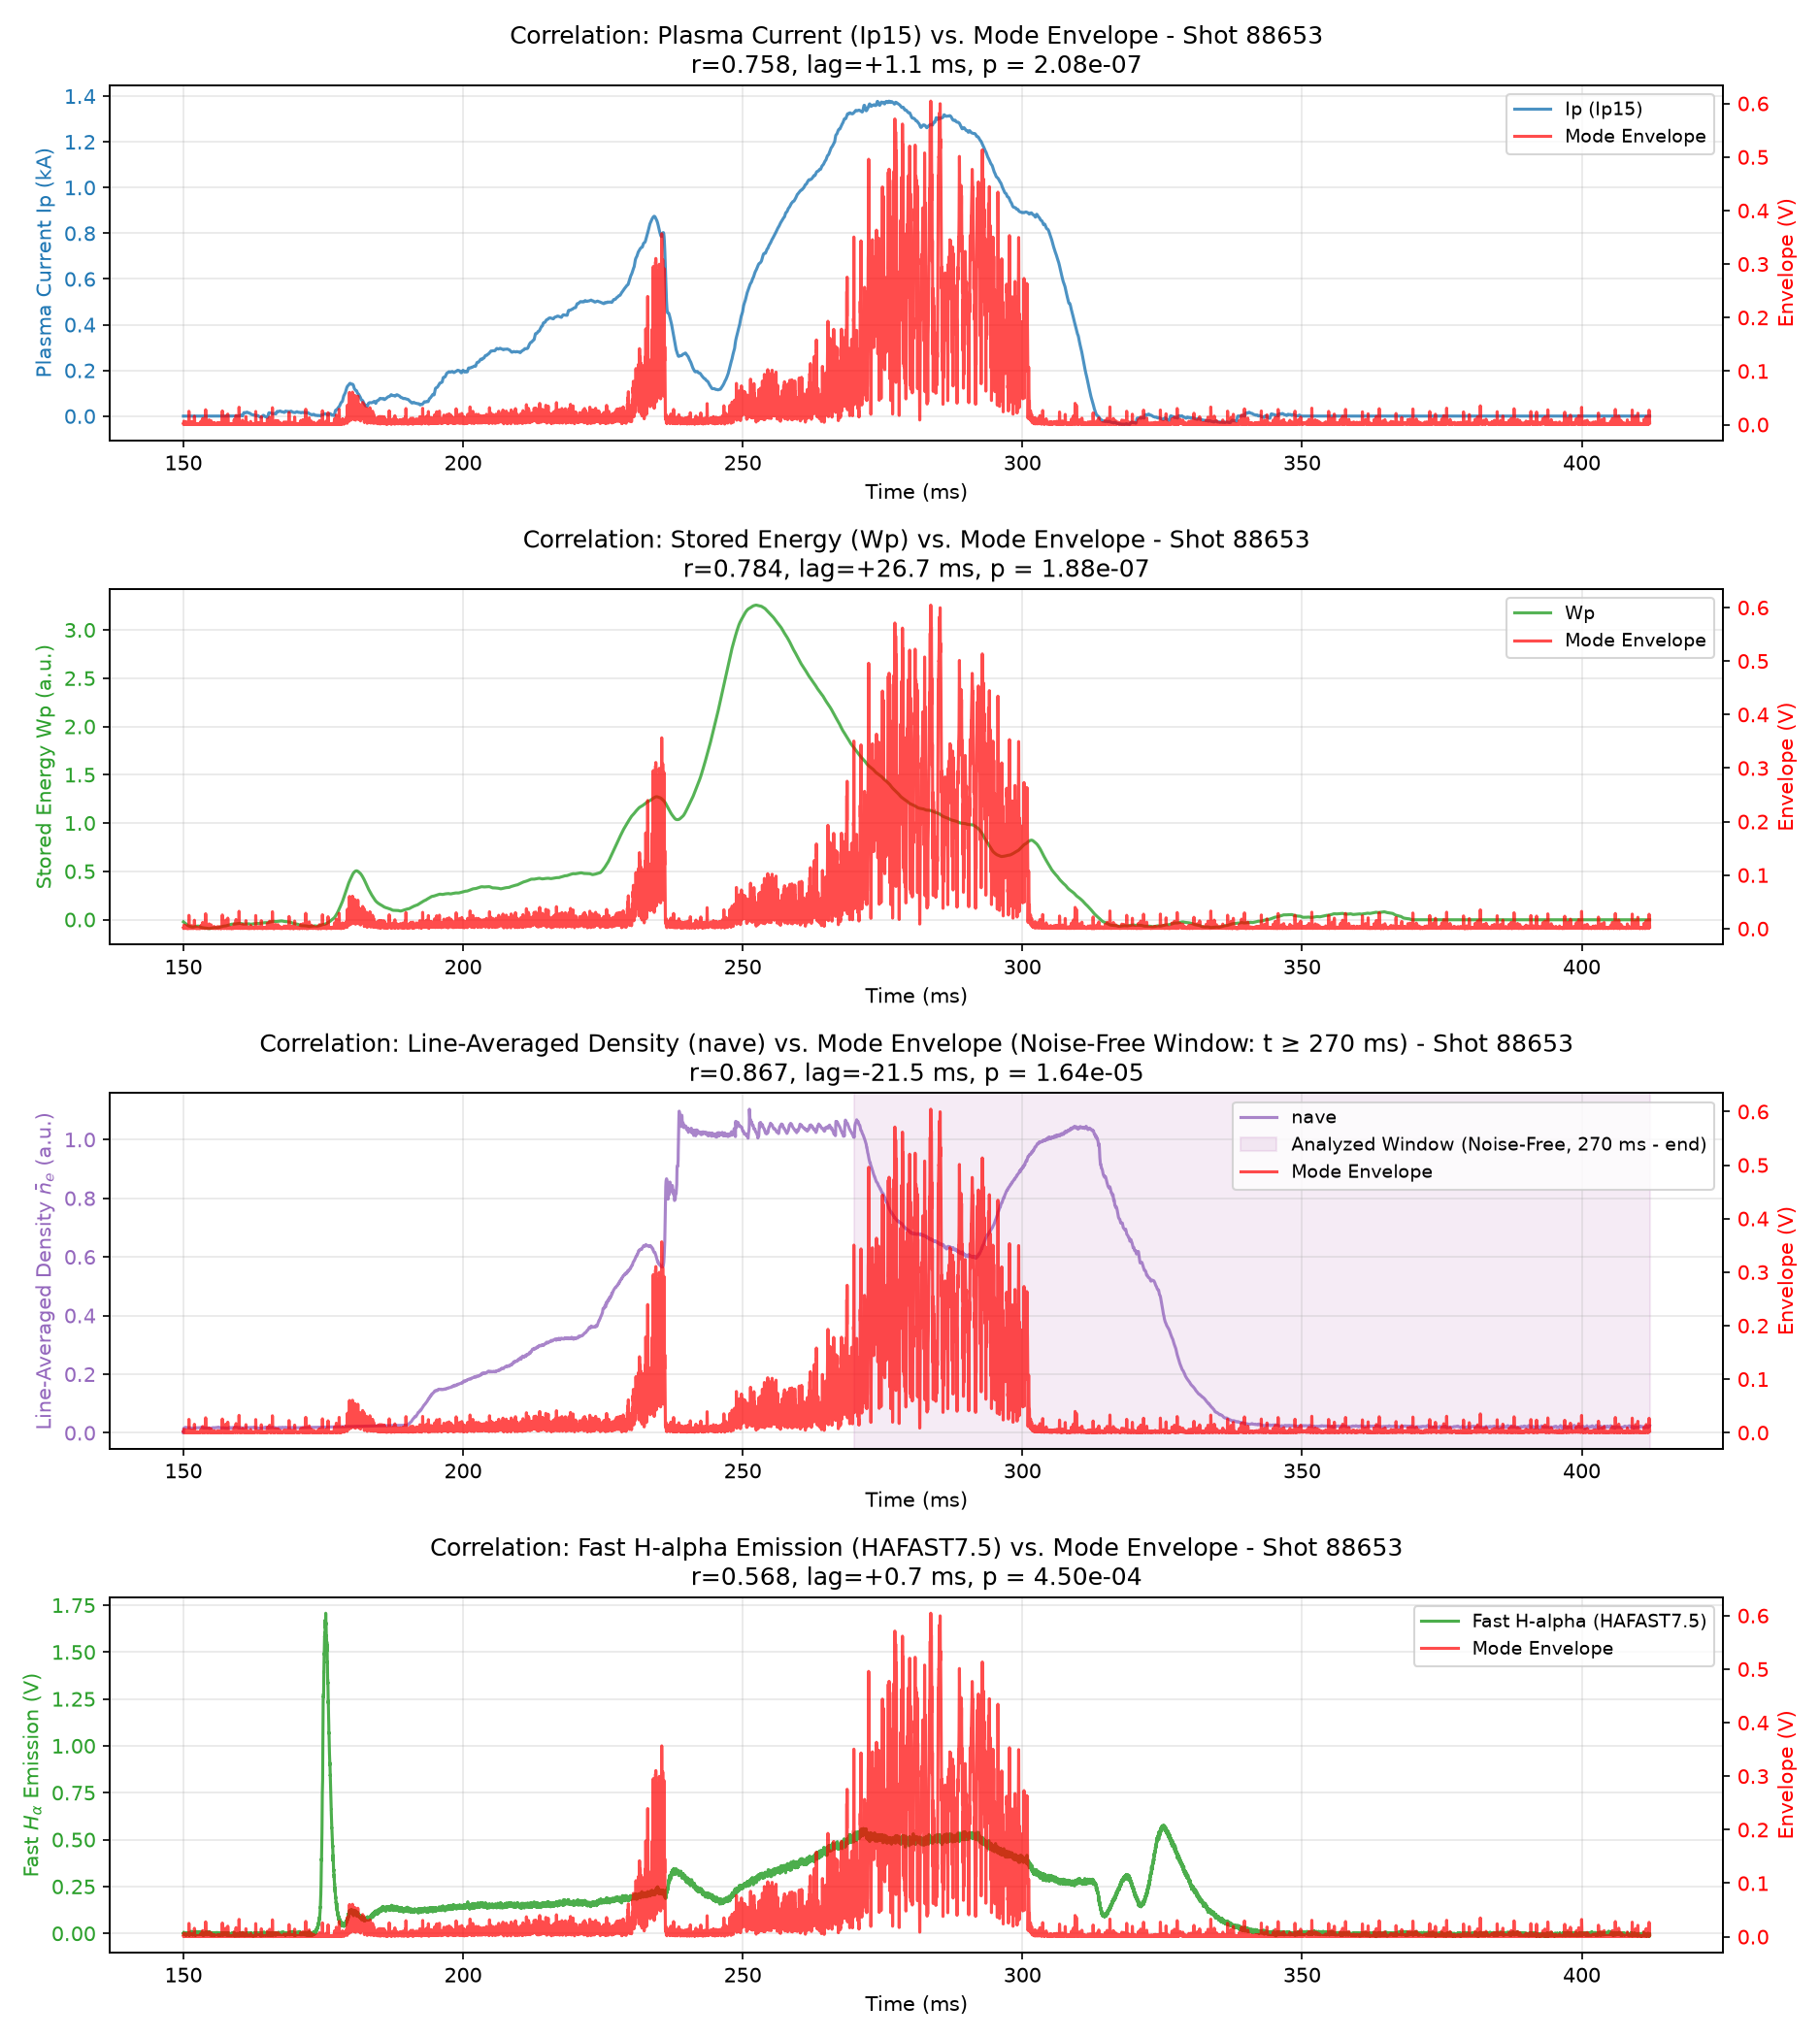
\includegraphics[height=0.85\textheight]{Images/obj2_dynamics_and_structure/mhd_analysis_objective2_88653_80_120kHz.png}
    \end{figure}
\end{frame}

\begin{frame}{Backup: Objective 2 -- Primary Band Heating Synchronization}
    \begin{figure}[h!]
        \centering
        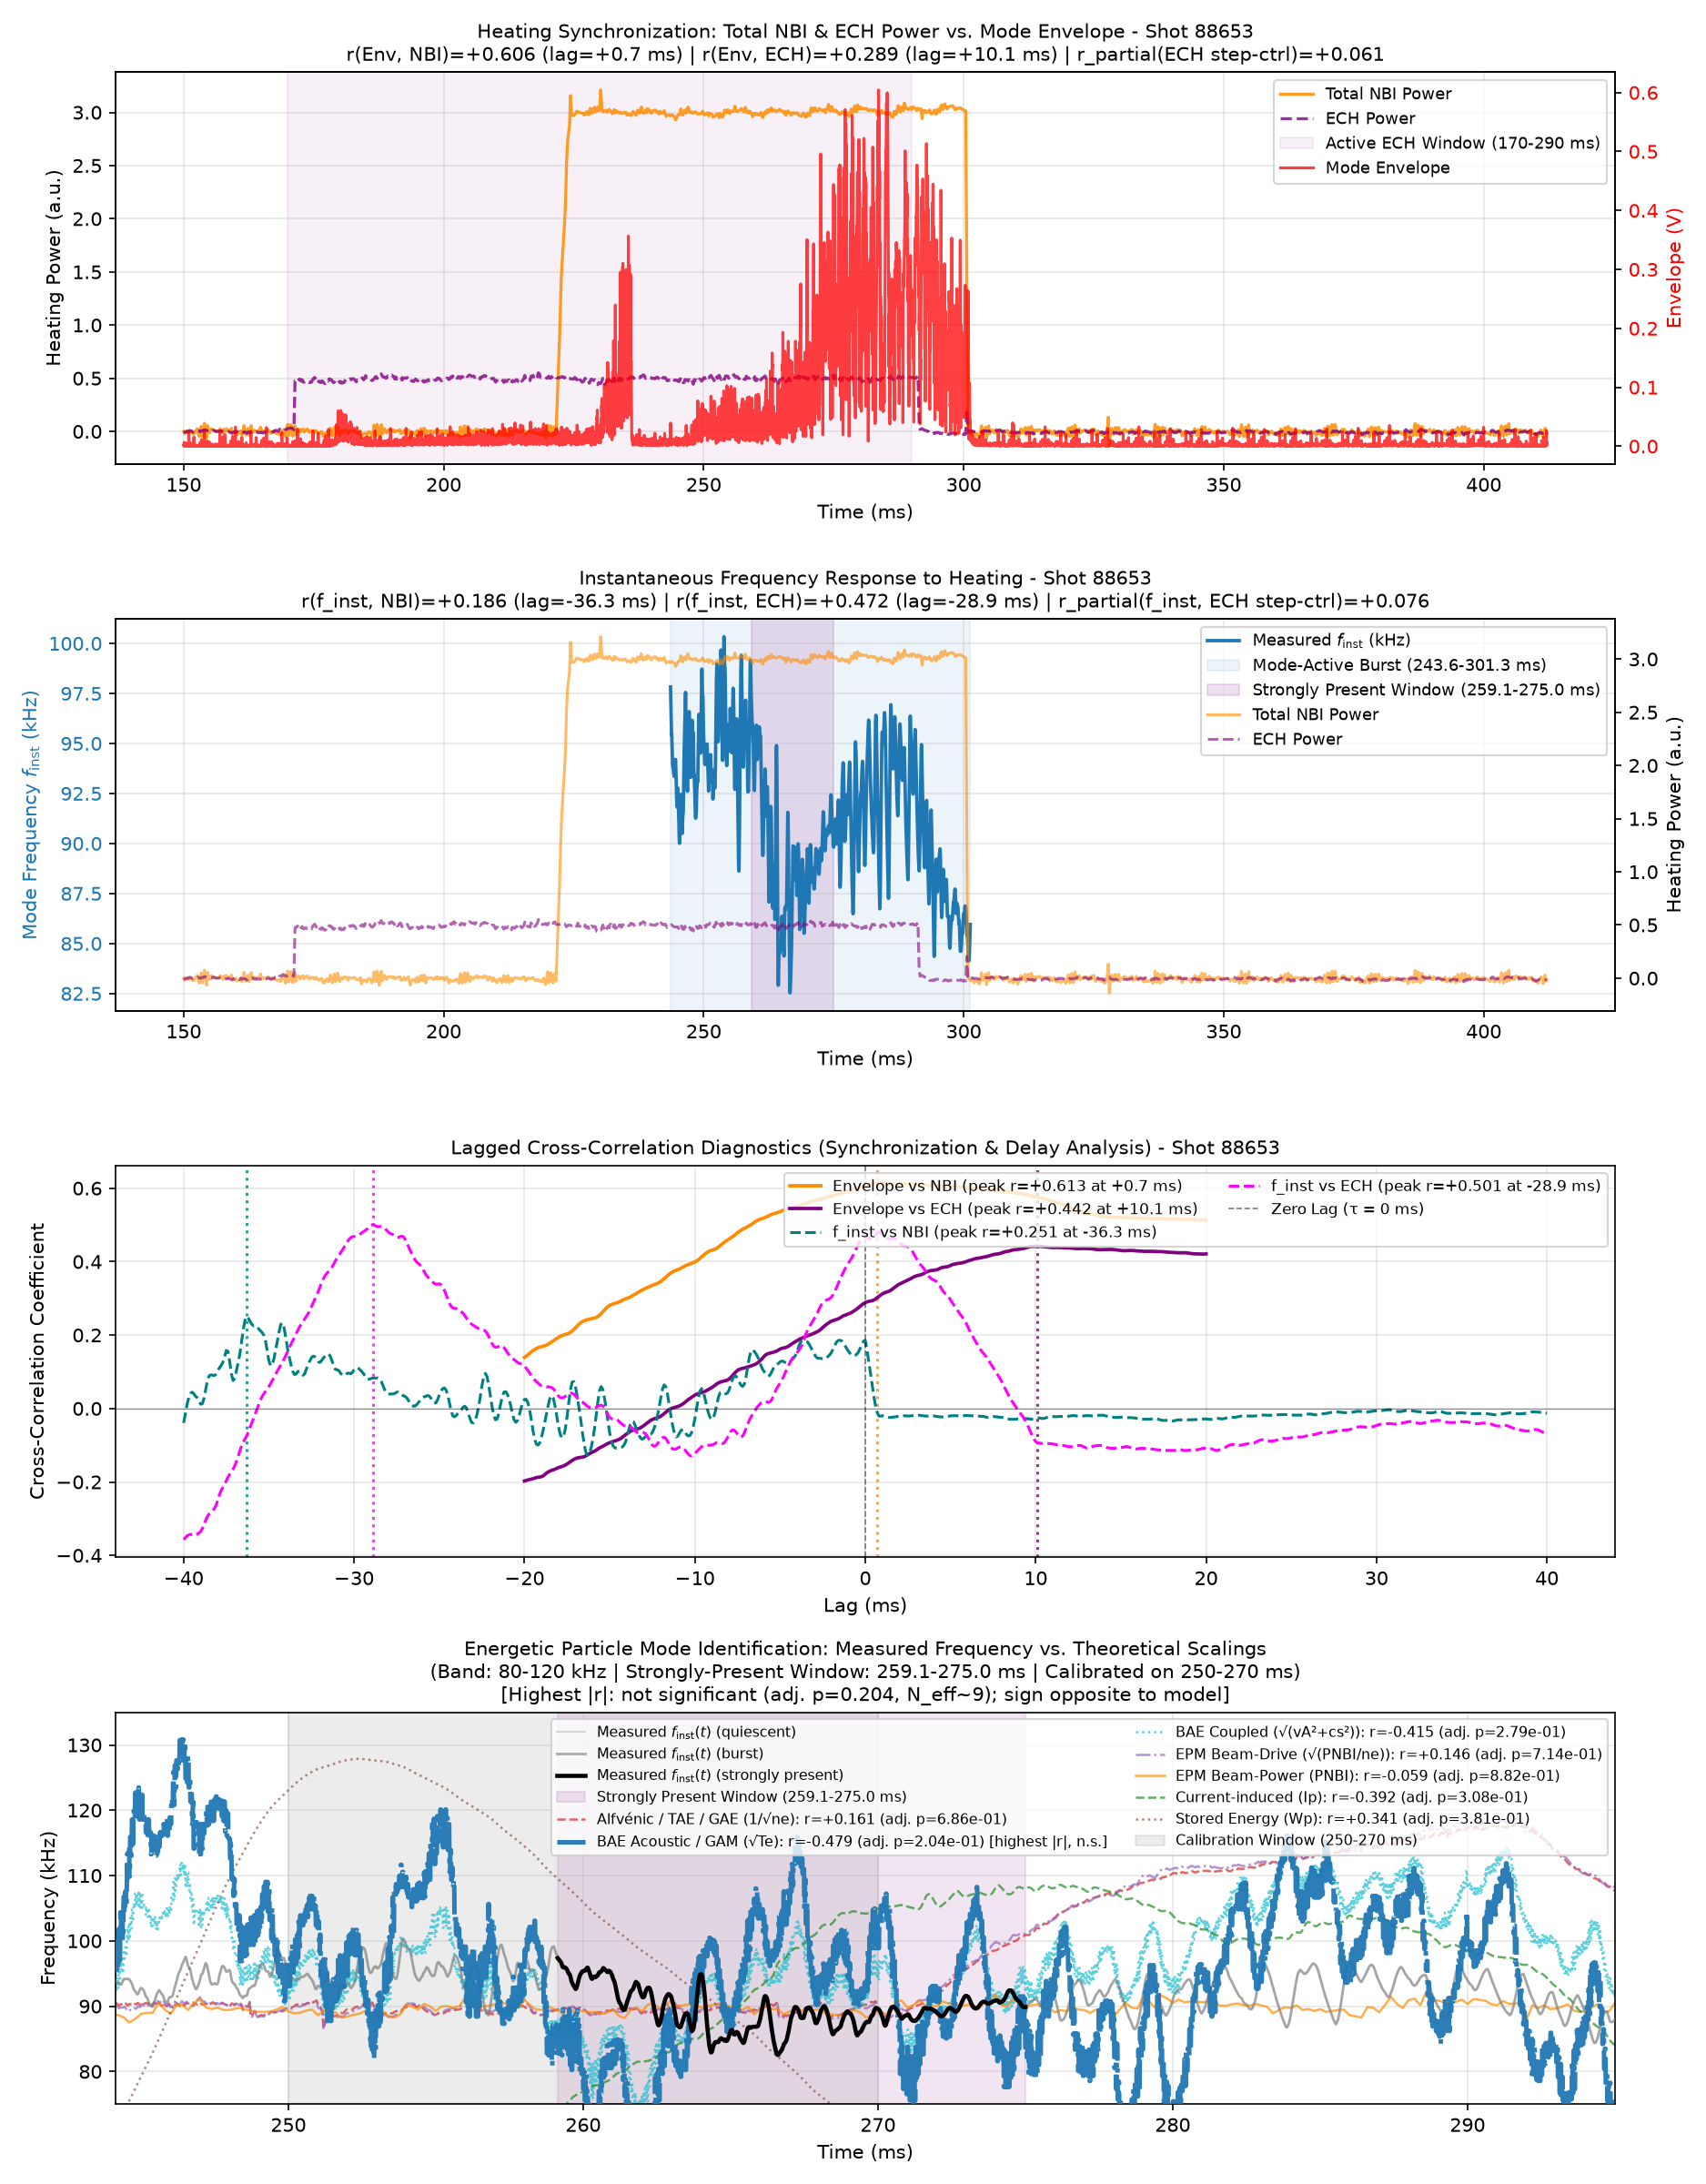
\includegraphics[height=0.85\textheight]{Images/obj2_dynamics_and_structure/mhd_analysis_objective2_heating_88653_80_120kHz.png}
    \end{figure}
\end{frame}

\begin{frame}{Backup: Objective 2 -- Secondary Band Poloidal Structure (Full Window)}
    \begin{figure}[h!]
        \centering
        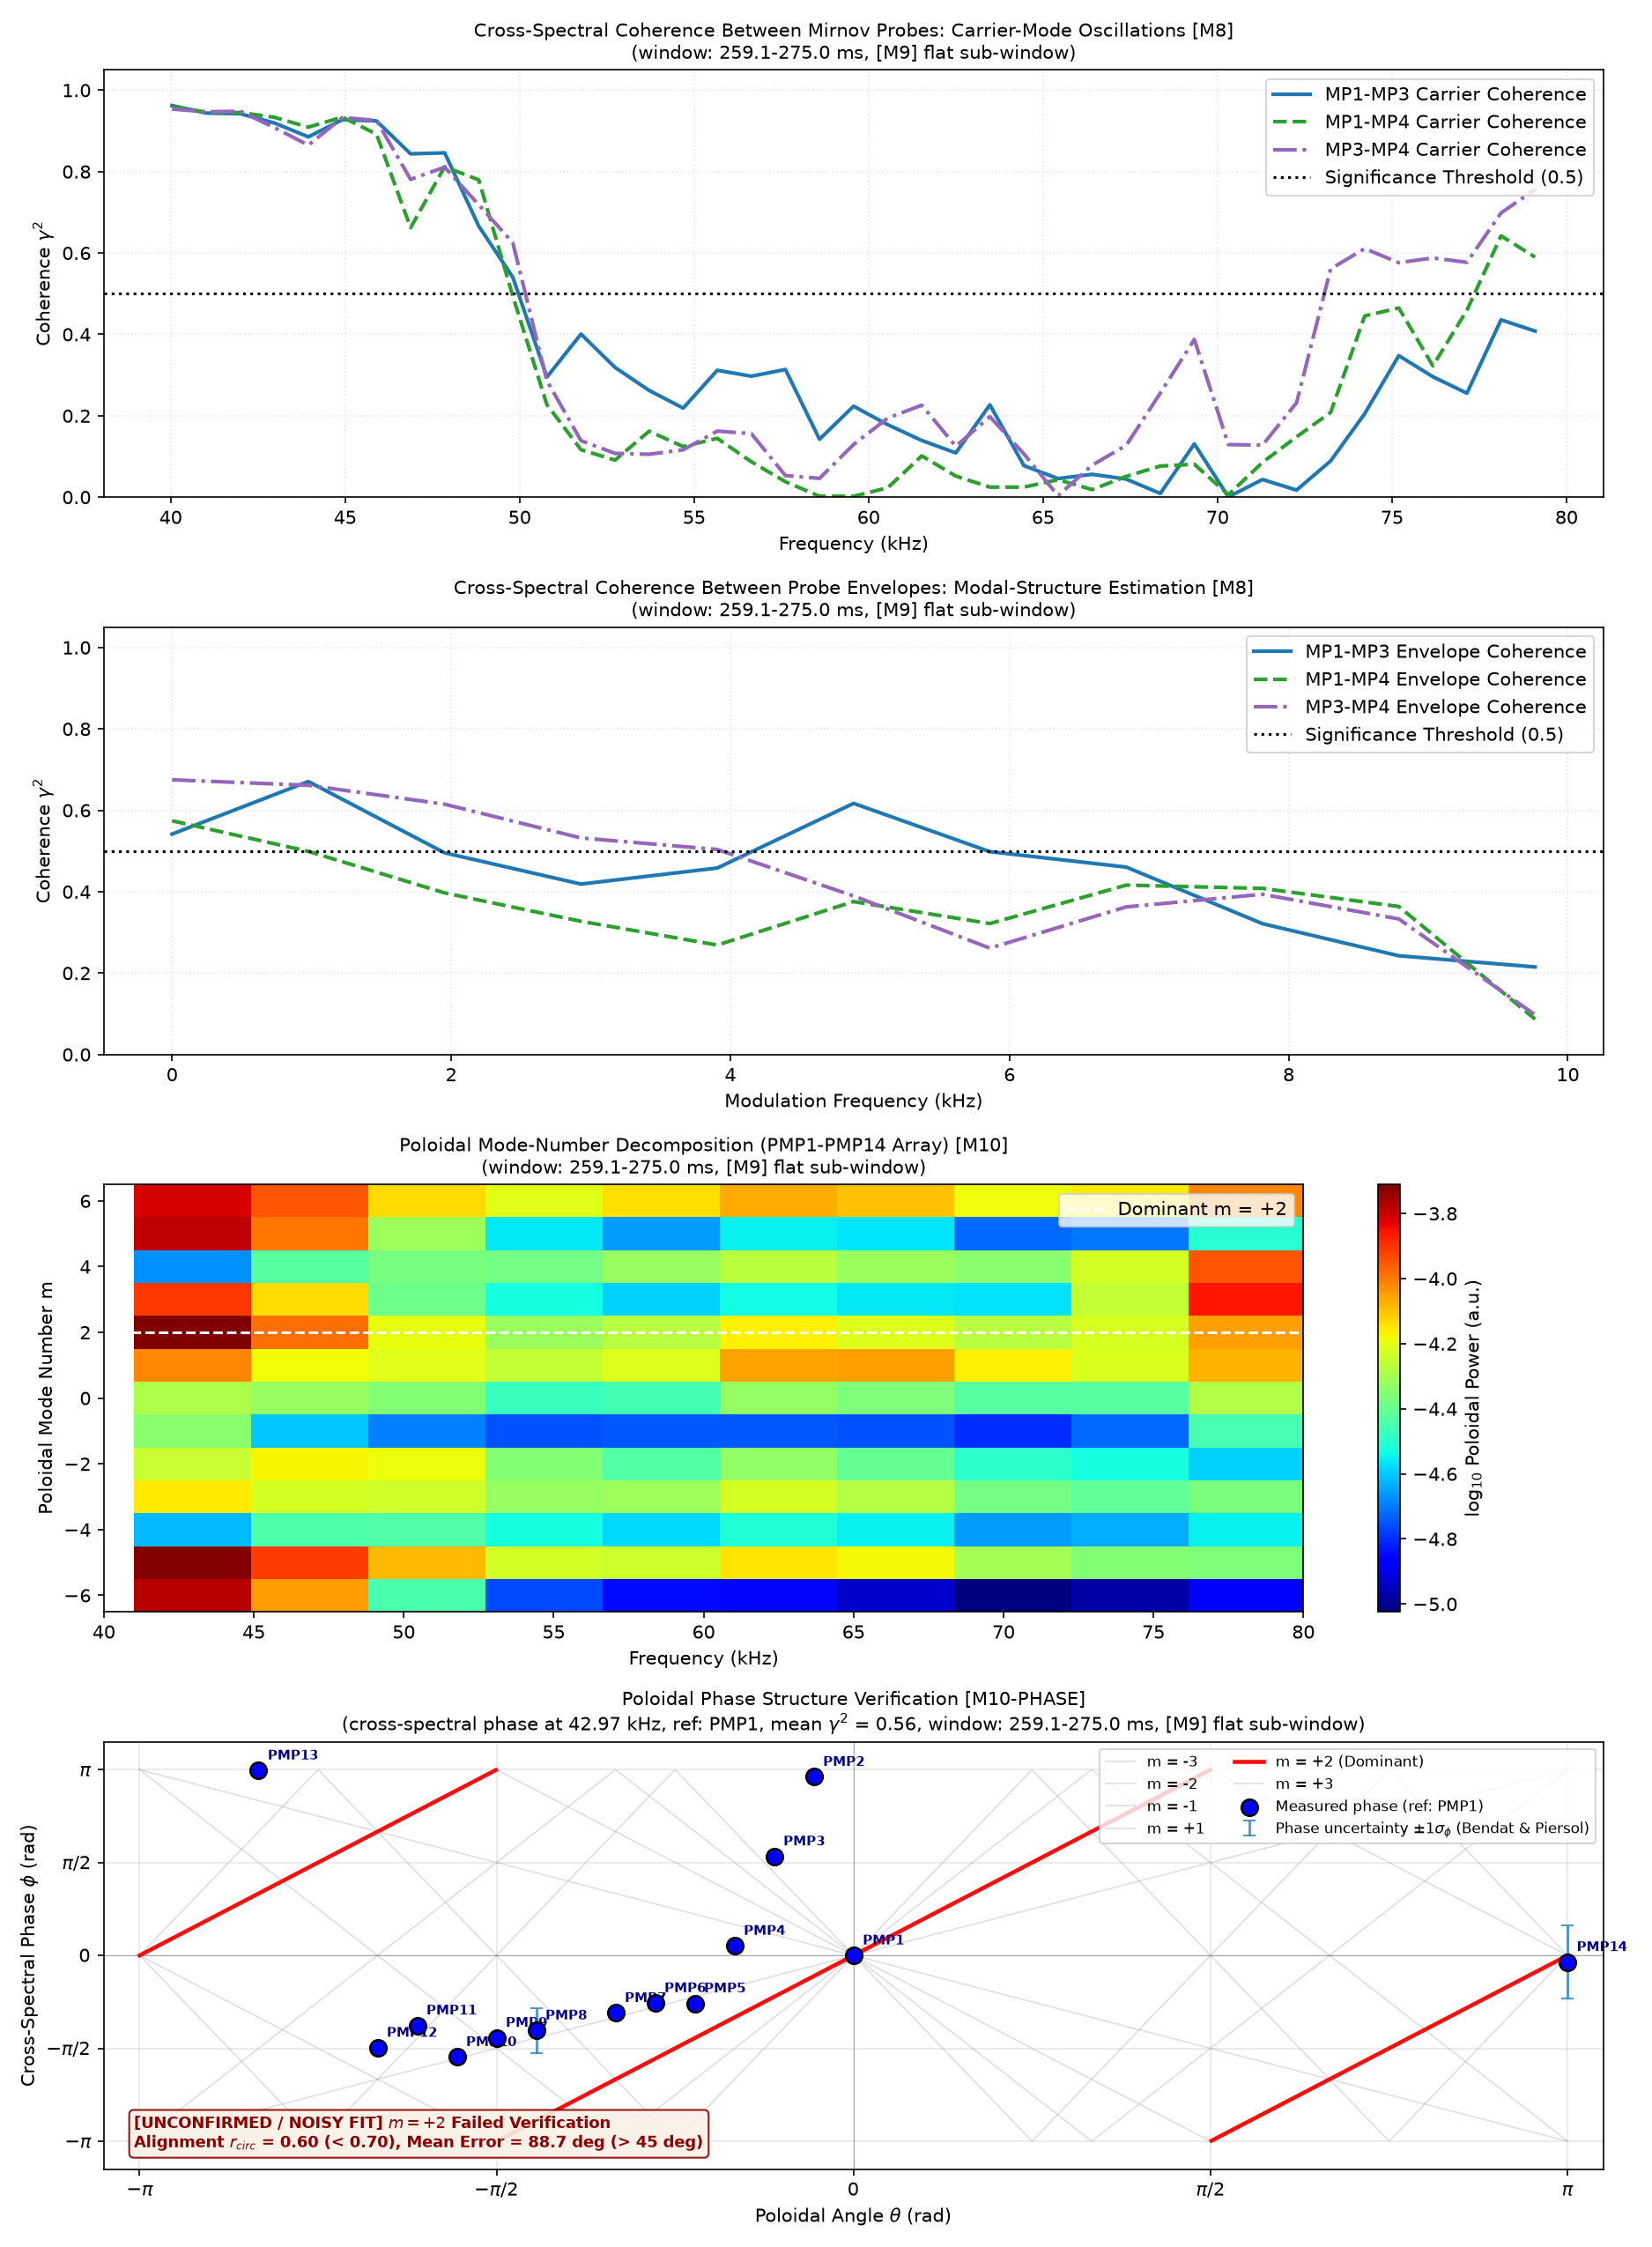
\includegraphics[width=0.85\textwidth,height=0.62\textheight,keepaspectratio]{Images/obj2_dynamics_and_structure/mhd_analysis_objective2_structure_88653_40_80kHz.png}
    \end{figure}
    \footnotesize
    Full ECH+NBI window (\SIrange{259.1}{291.3}{ms}), companion to the Primary full-window
    structure on the main Objective 2 slide. Consistent with the tentative status
    reported there: $m$ is not stable across the ECH+NBI/NBI-only split (see next slide).
\end{frame}

\begin{frame}{Backup: Objective 2 Comparative -- Secondary Band Spatial Structure}
    \begin{columns}[T]
        \begin{column}{0.5\textwidth}
            \centering ECH+NBI\\
            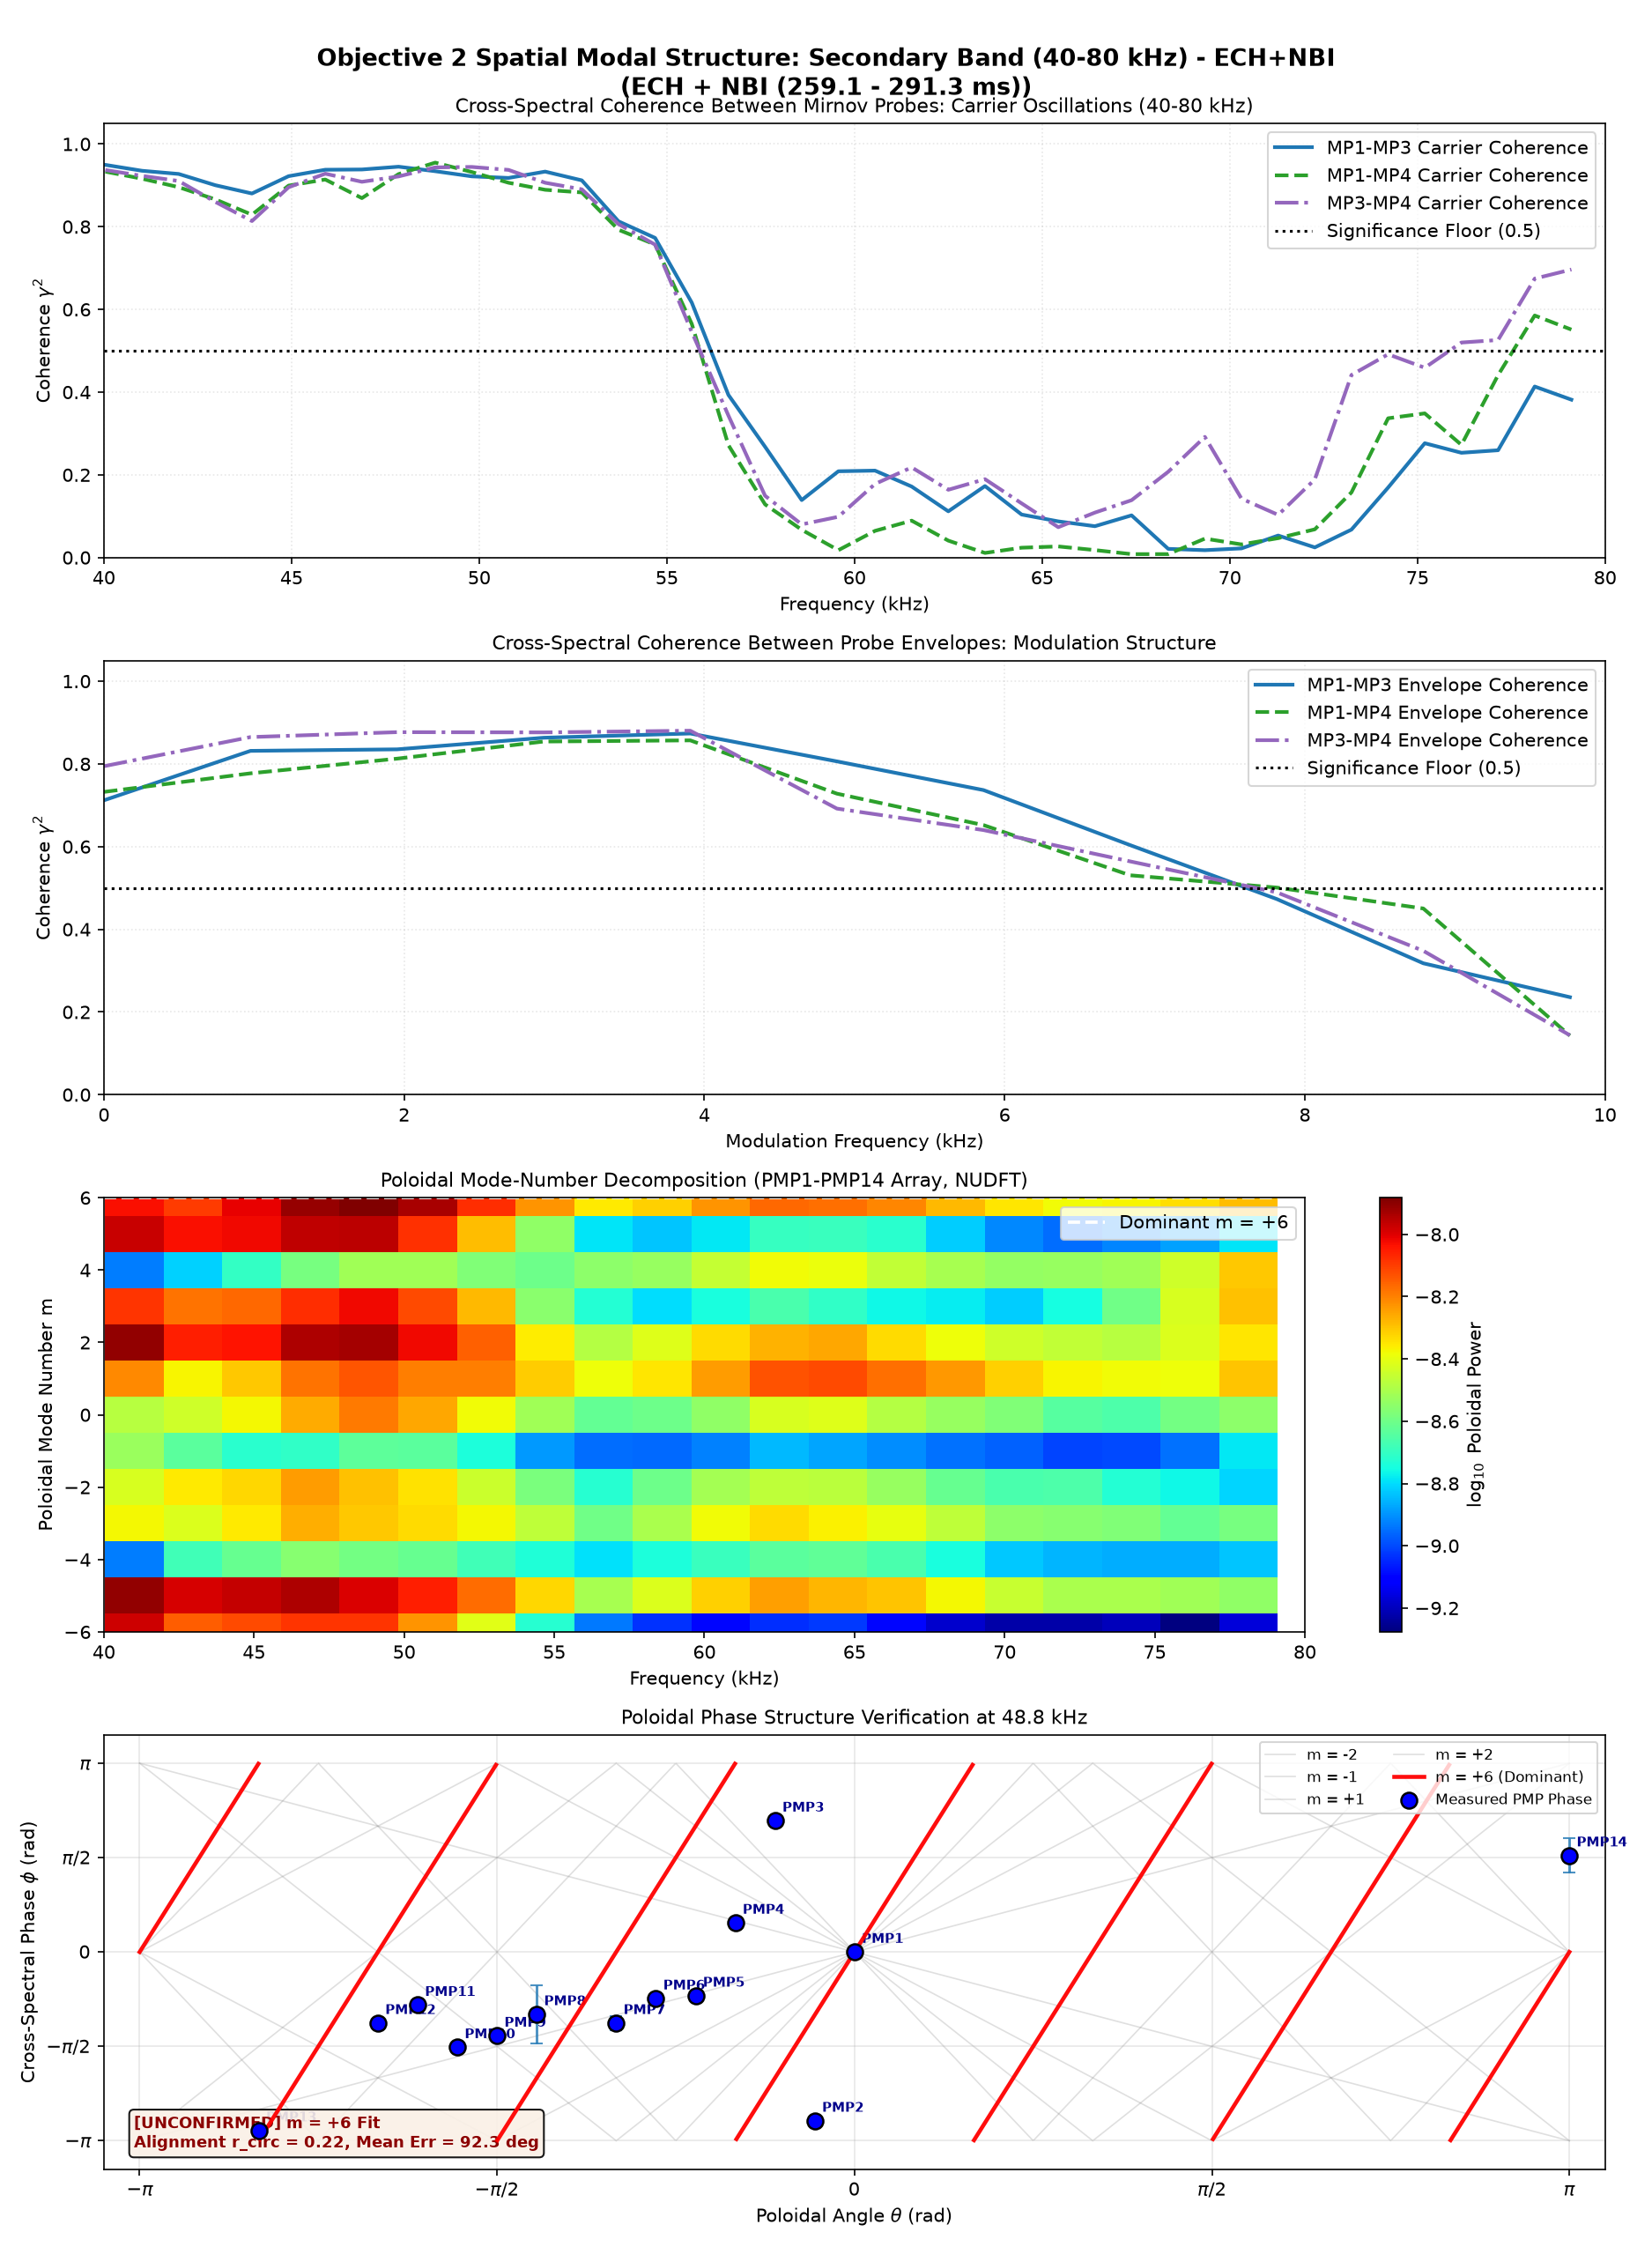
\includegraphics[width=\textwidth,height=0.66\textheight,keepaspectratio]{Images/heating_phase_comparison/mhd_analysis_objective2_structure_88653_40_80kHz_ECH_NBI.png}
        \end{column}
        \begin{column}{0.5\textwidth}
            \centering NBI-only\\
            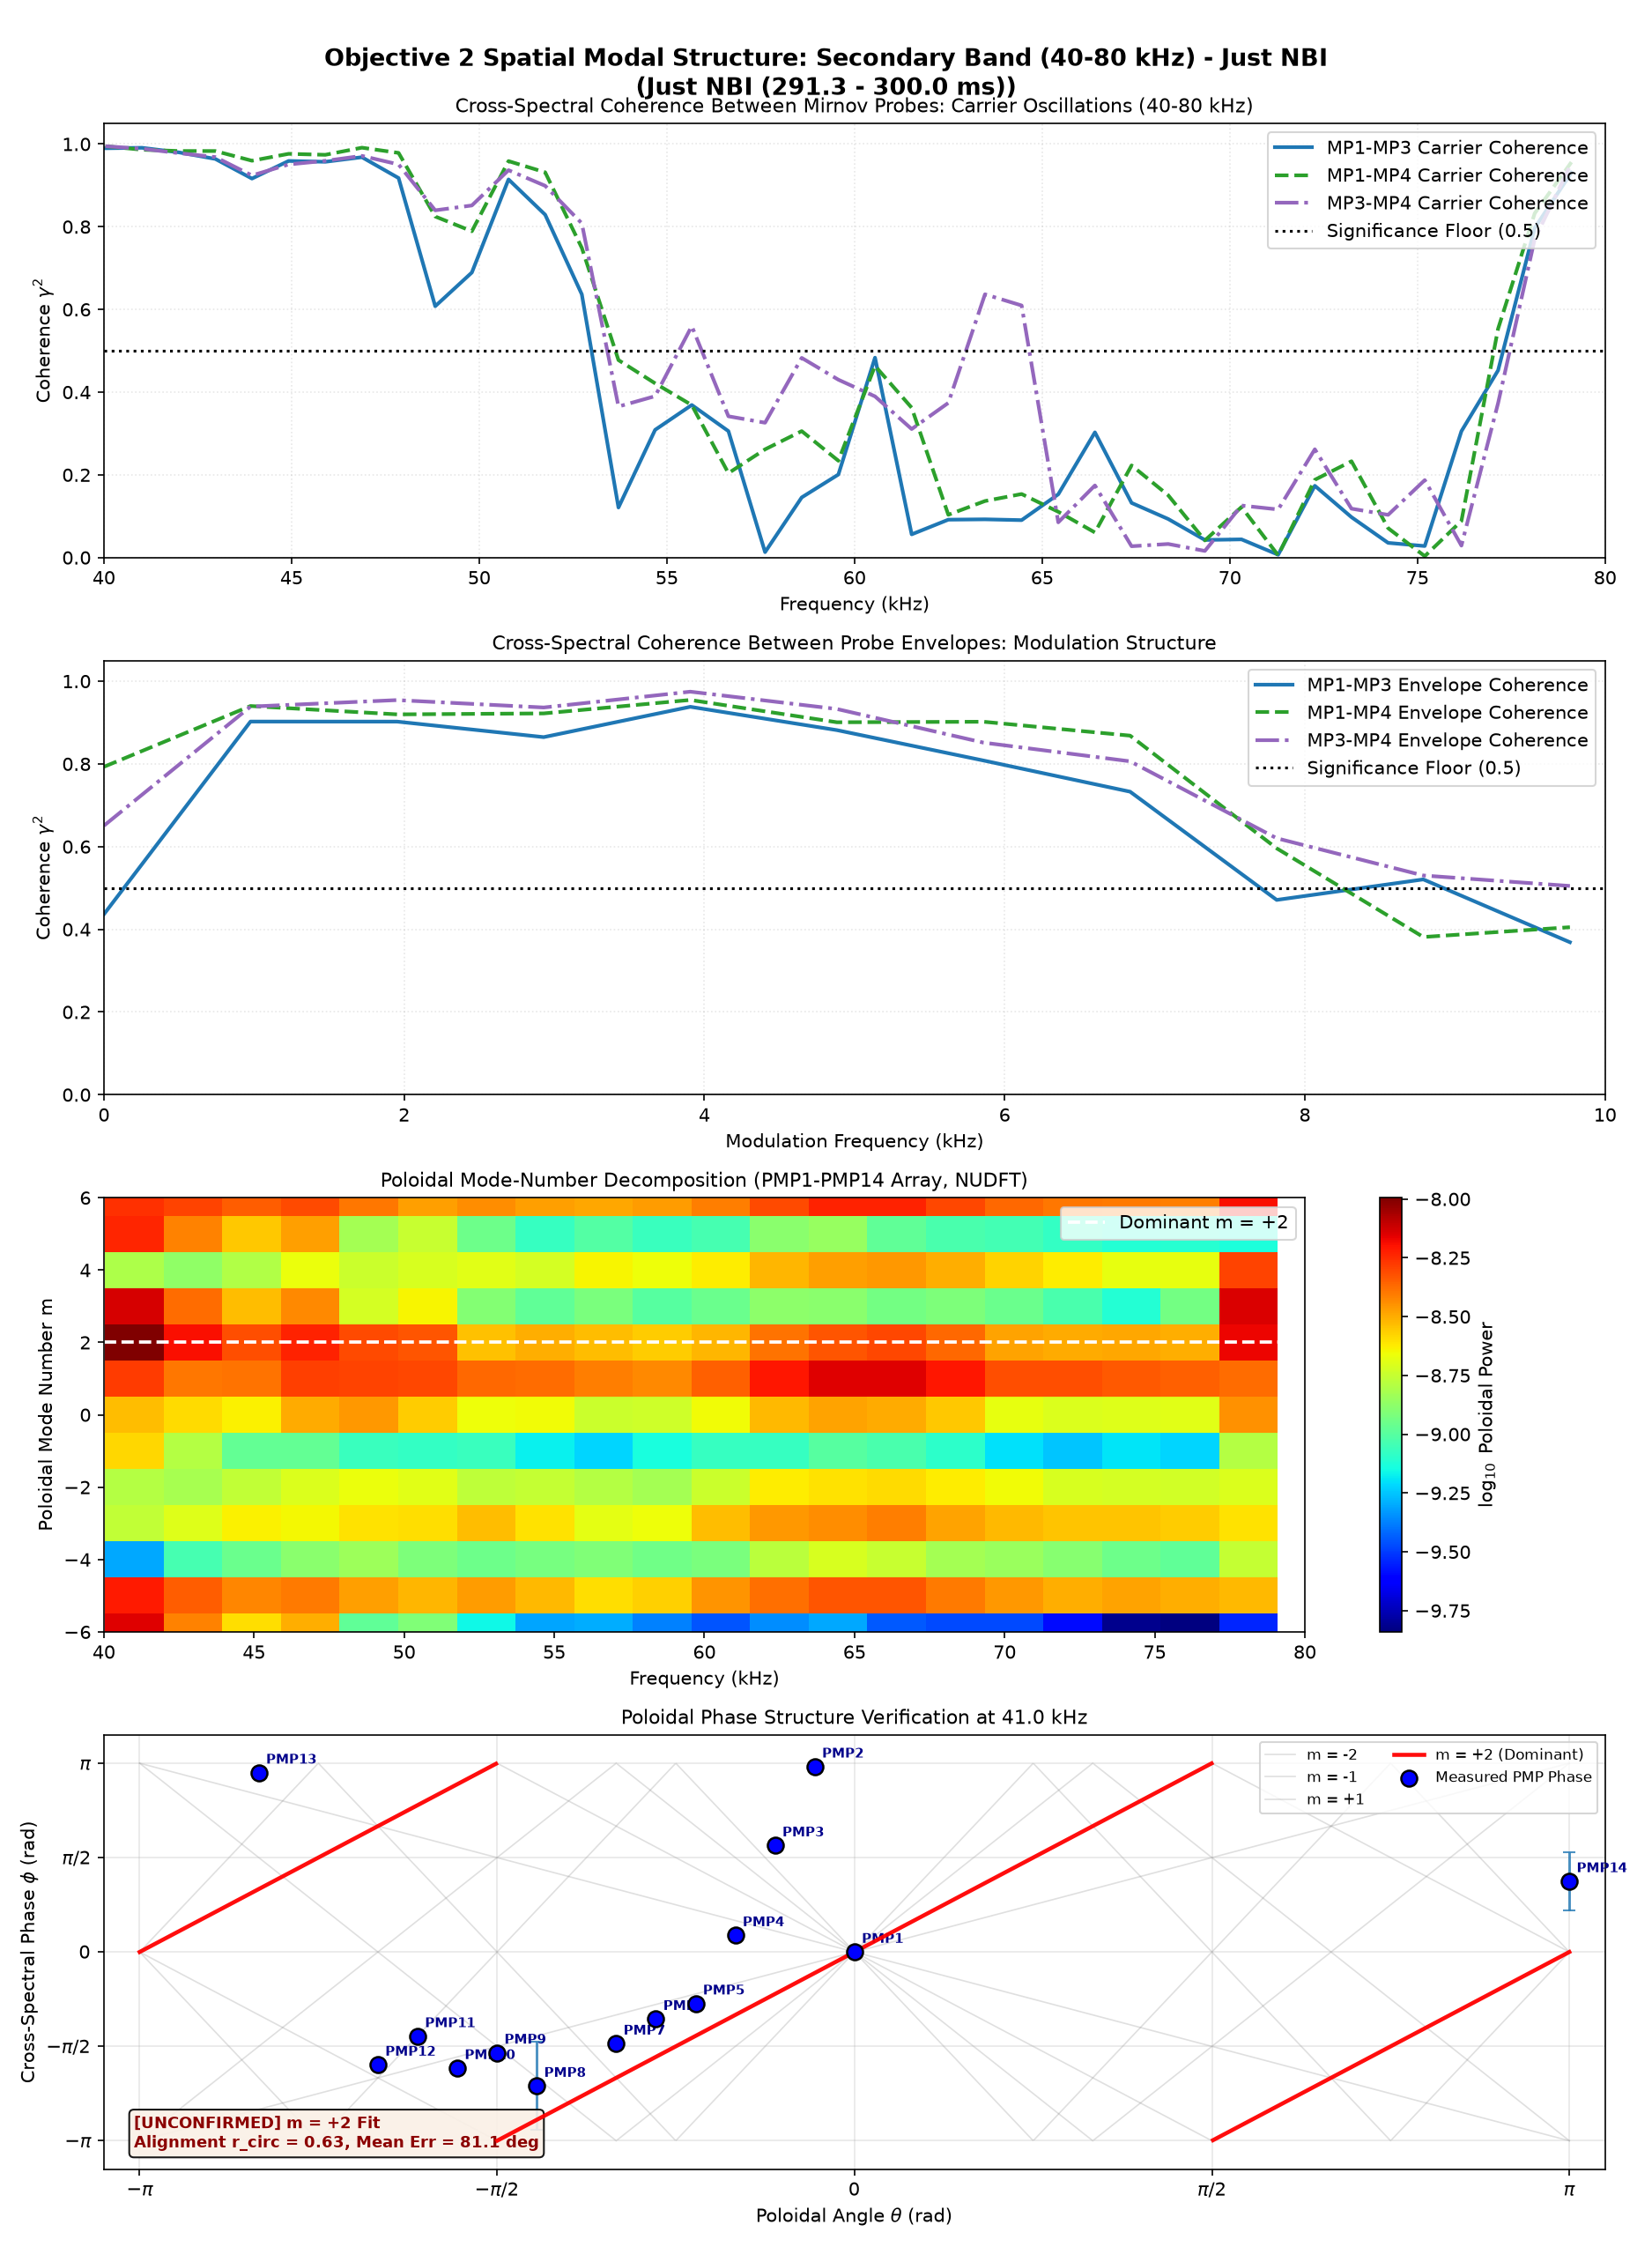
\includegraphics[width=\textwidth,height=0.66\textheight,keepaspectratio]{Images/heating_phase_comparison/mhd_analysis_objective2_structure_88653_40_80kHz_NBI_only.png}
        \end{column}
    \end{columns}
\end{frame}

\begin{frame}{Backup: Objective 2 Comparative -- Primary Band Spatial Structure}
    \begin{columns}[T]
        \begin{column}{0.5\textwidth}
            \centering ECH+NBI\\
            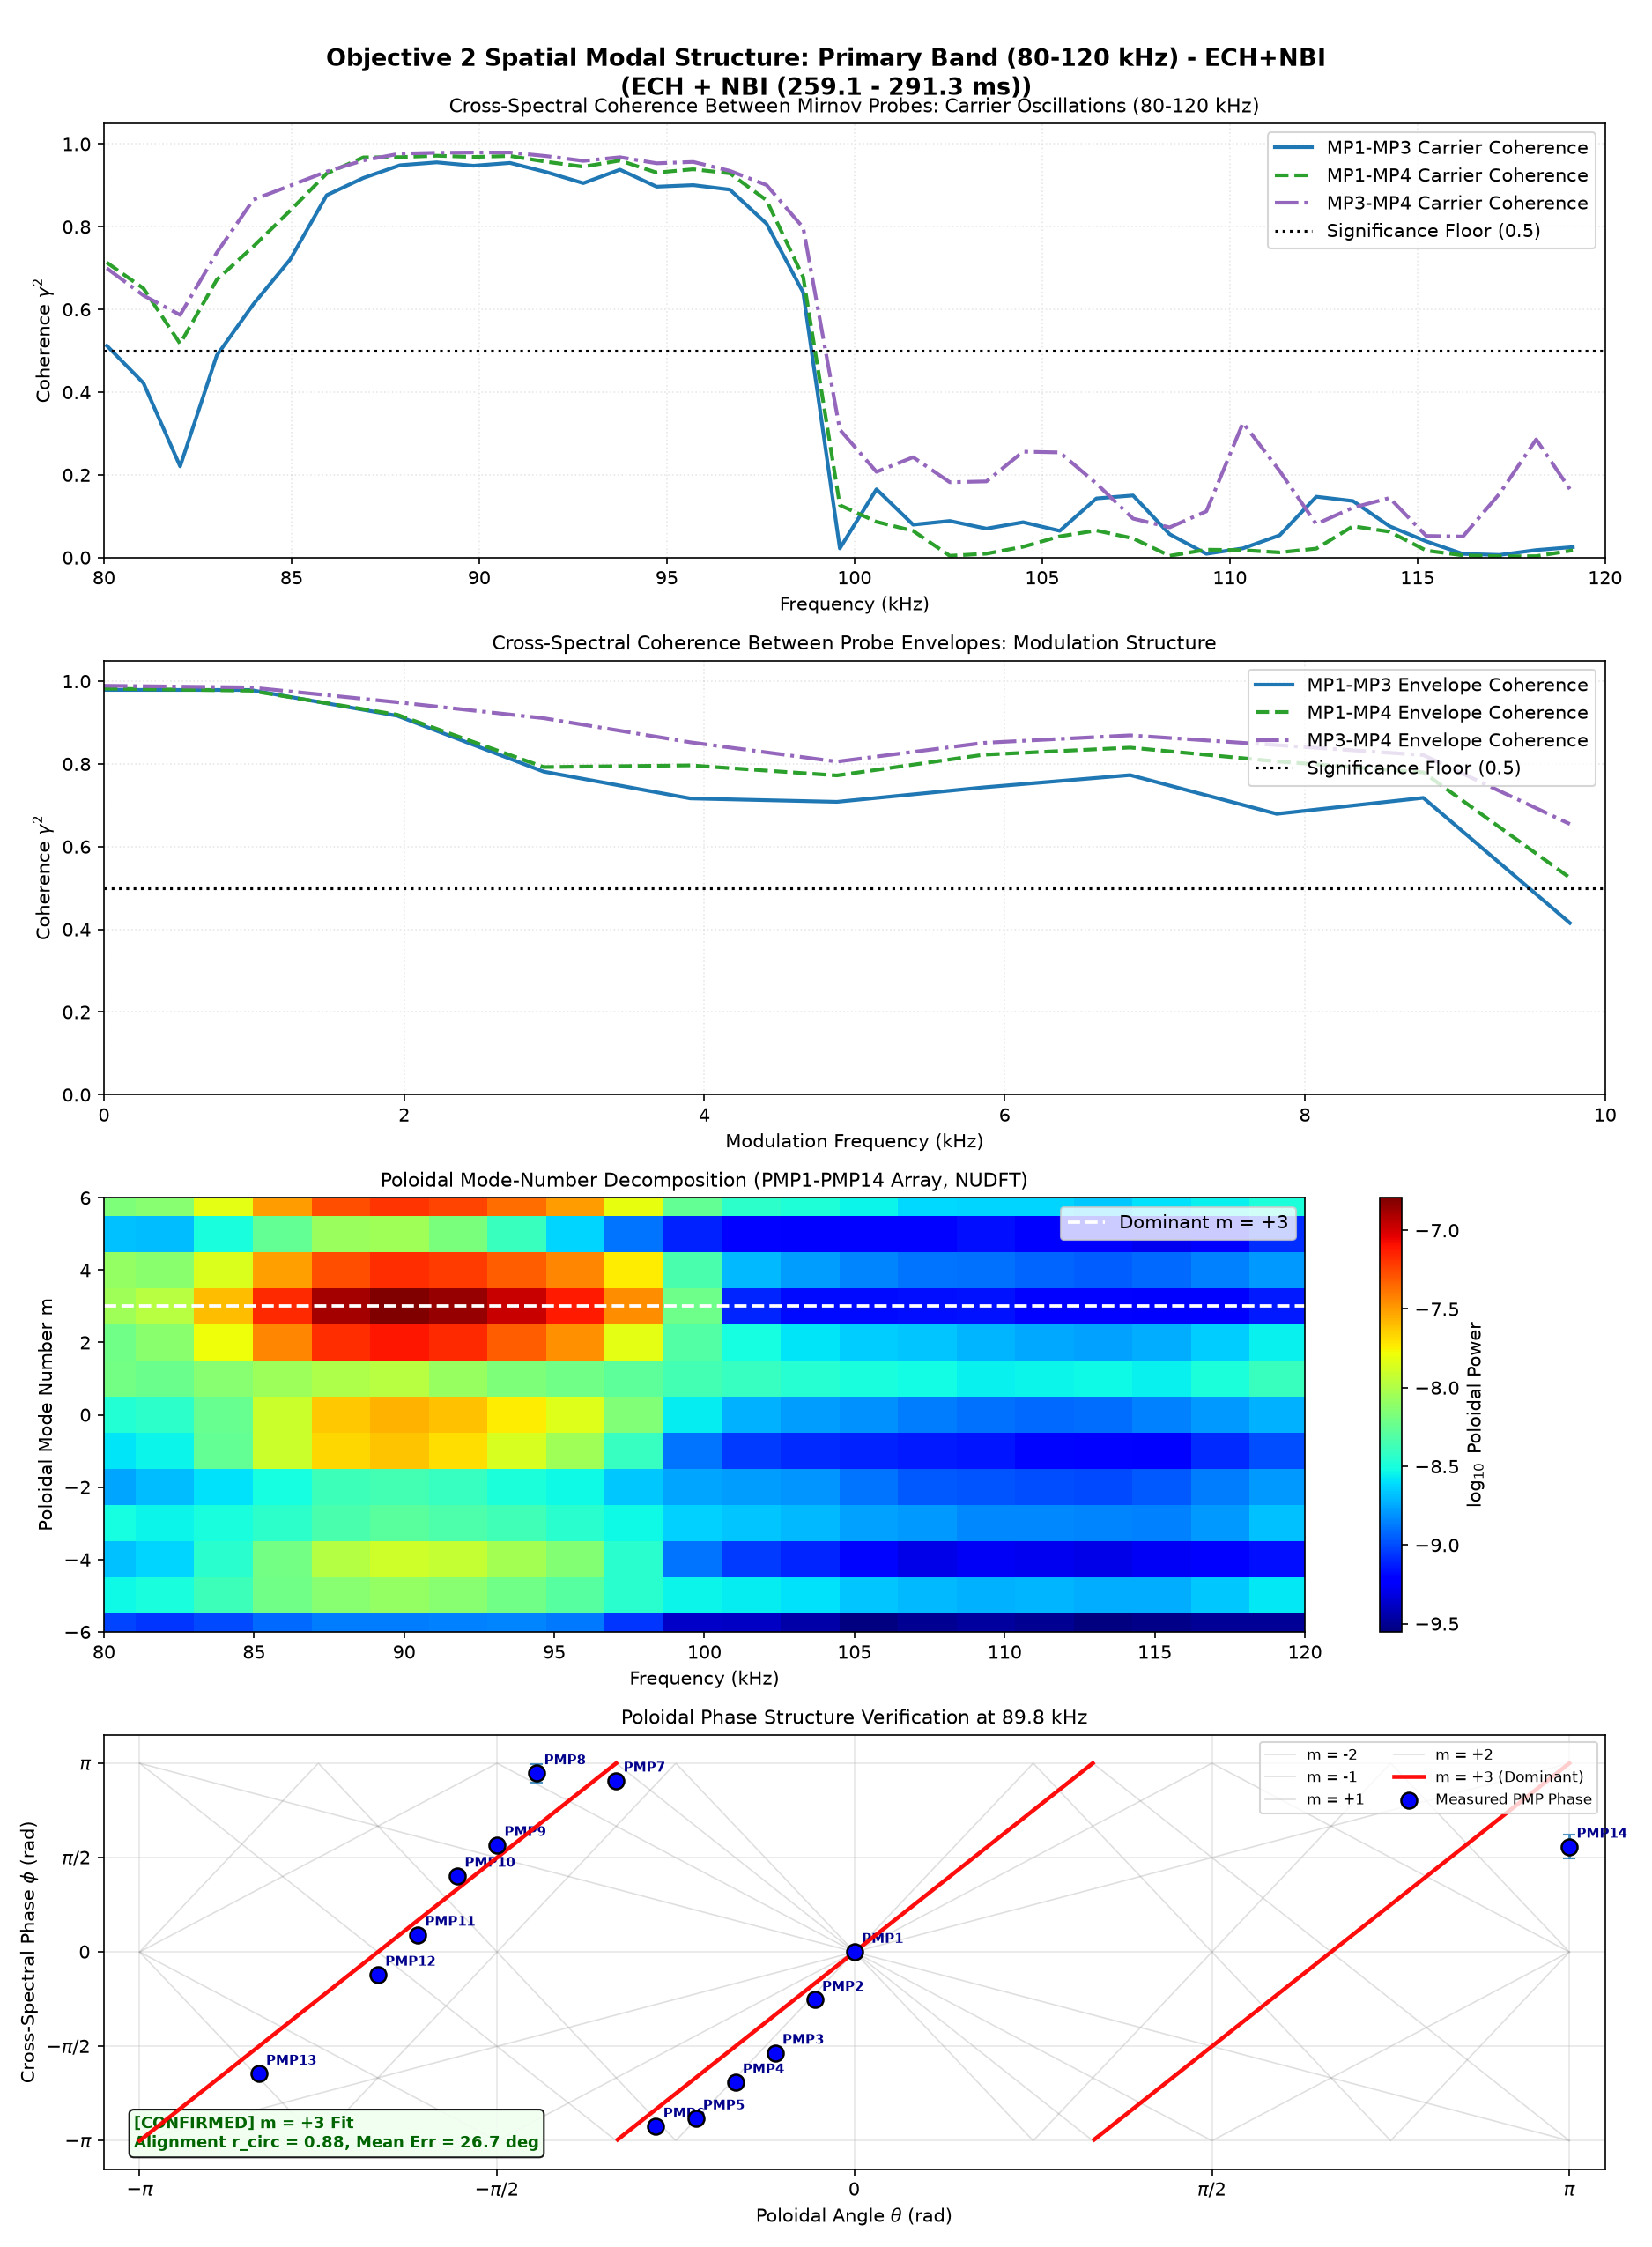
\includegraphics[width=\textwidth,height=0.66\textheight,keepaspectratio]{Images/heating_phase_comparison/mhd_analysis_objective2_structure_88653_80_120kHz_ECH_NBI.png}
        \end{column}
        \begin{column}{0.5\textwidth}
            \centering NBI-only\\
            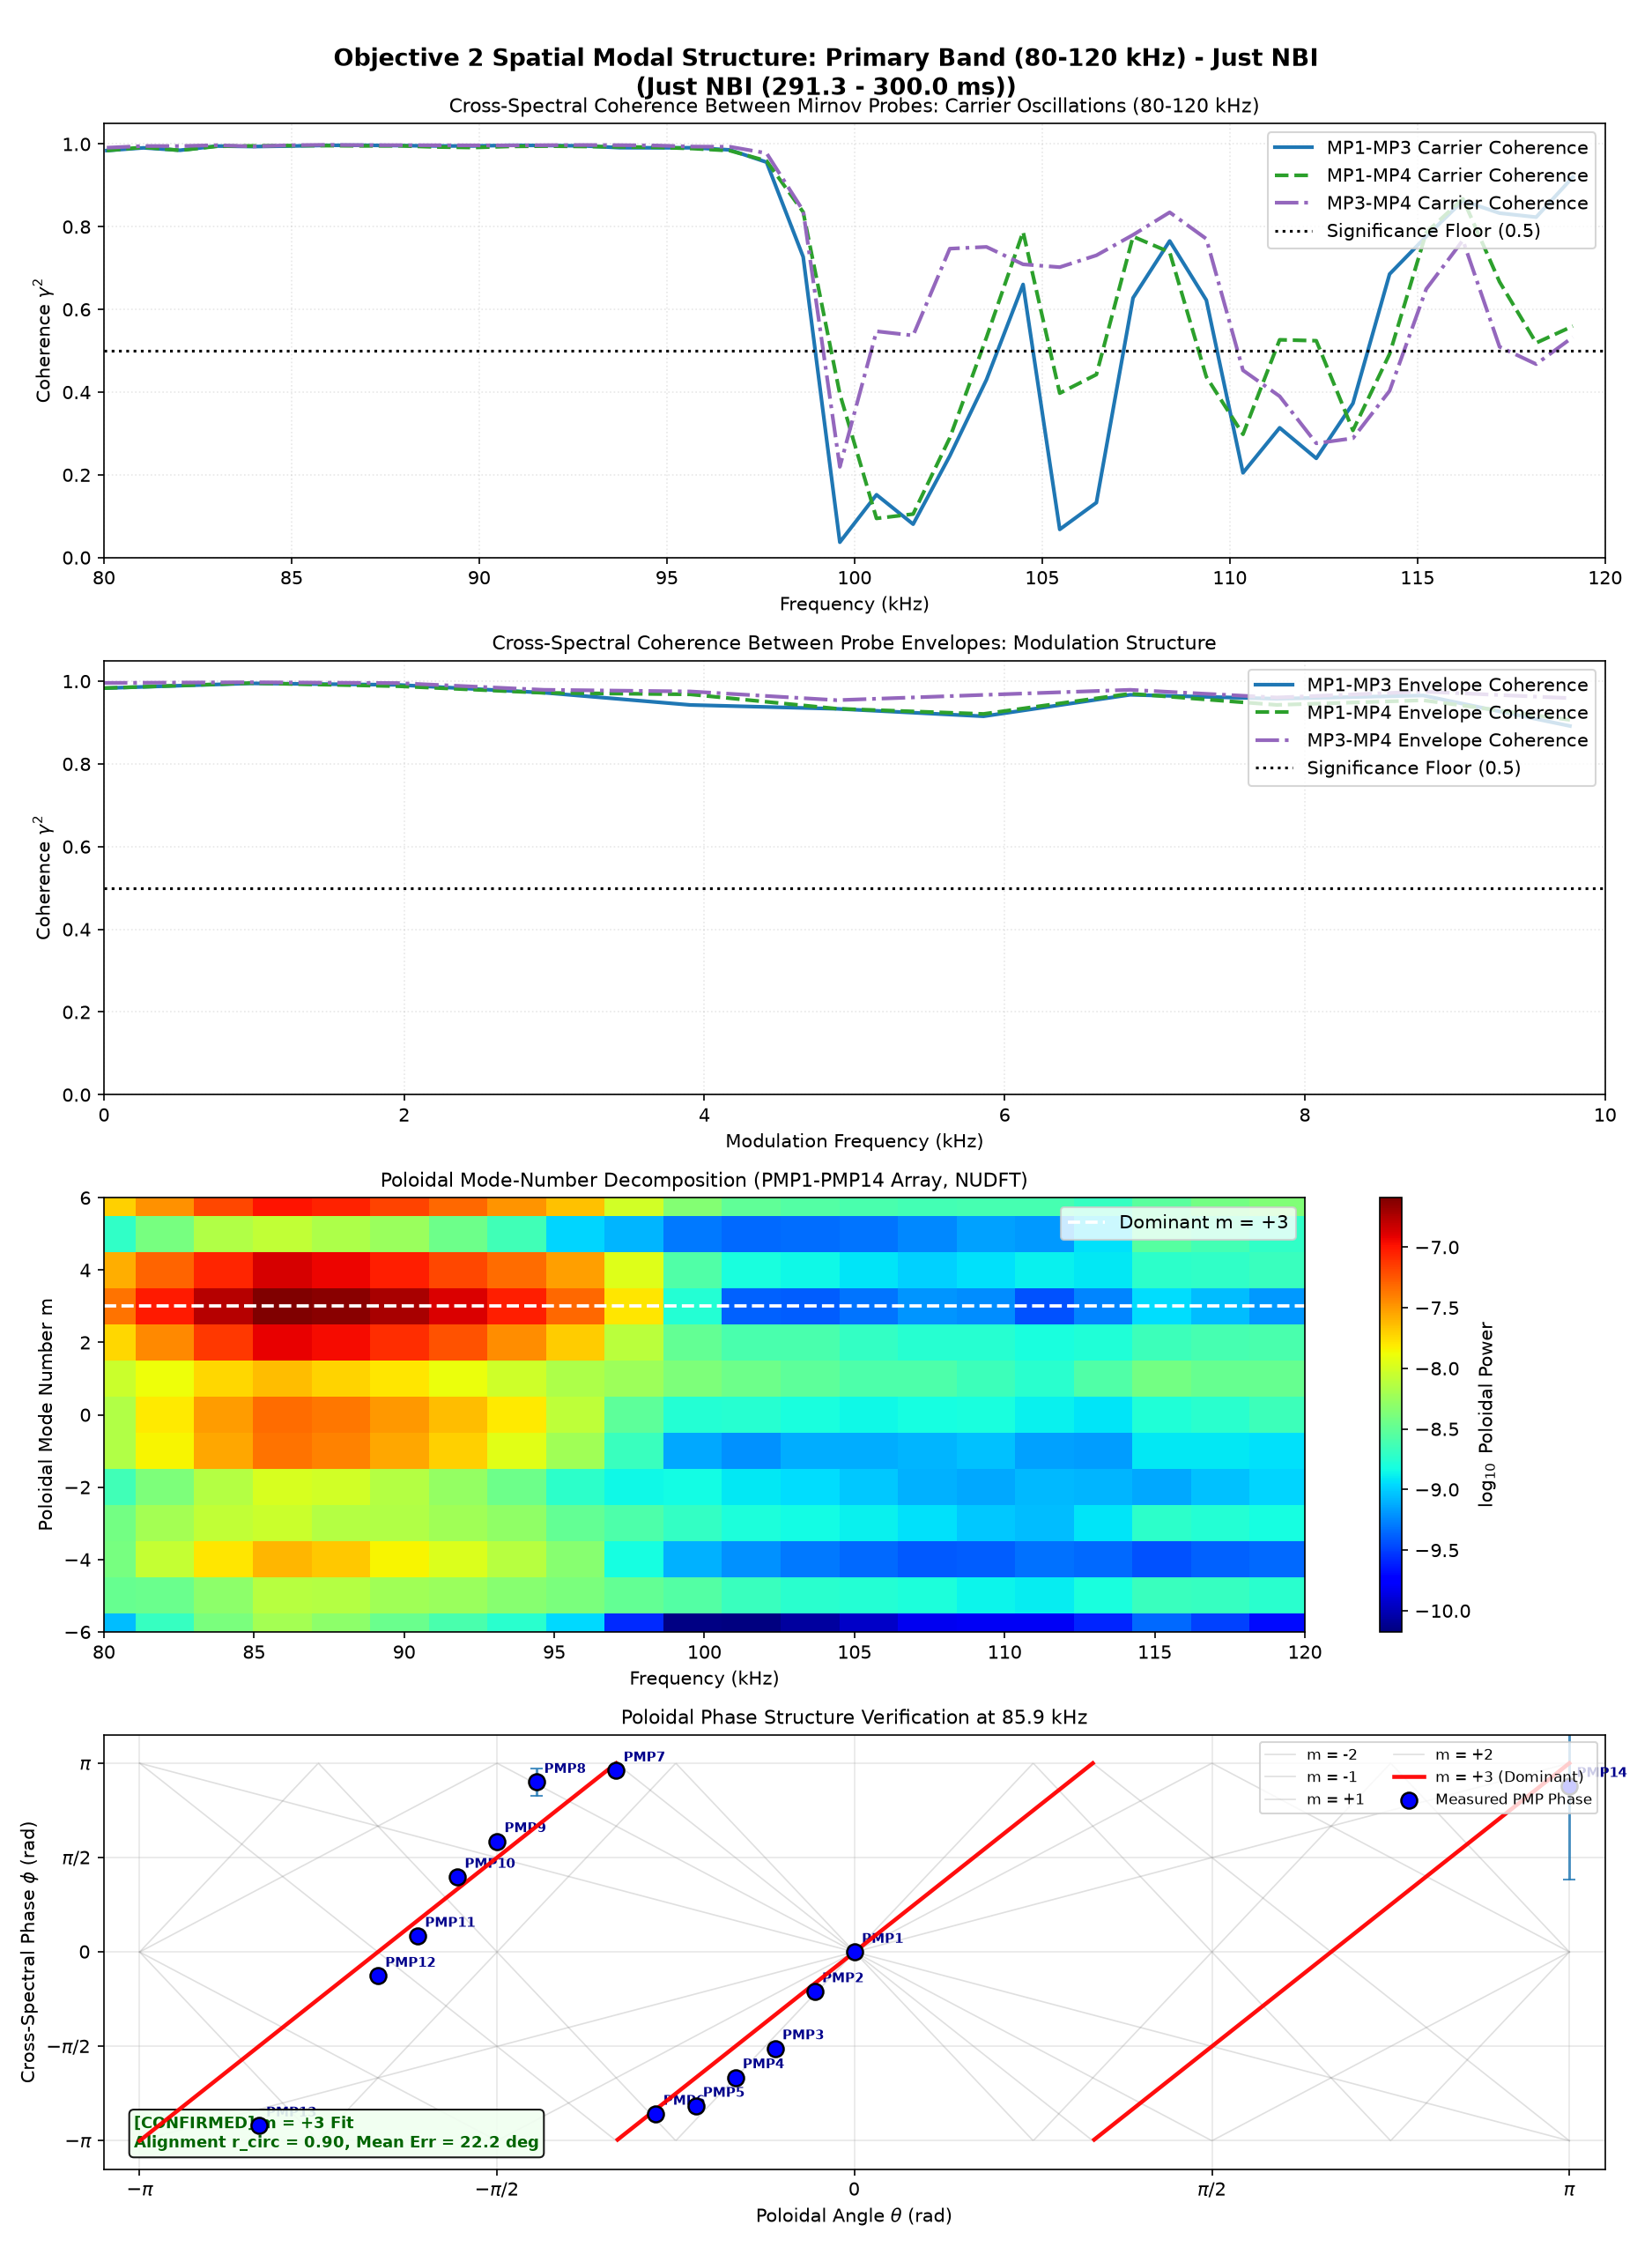
\includegraphics[width=\textwidth,height=0.66\textheight,keepaspectratio]{Images/heating_phase_comparison/mhd_analysis_objective2_structure_88653_80_120kHz_NBI_only.png}
        \end{column}
    \end{columns}
\end{frame}

\begin{frame}{Backup: Objective 2 Comparative -- Poloidal Mode Number \& Phase}
    \small
    \centering
    \begin{tabular}{llccccc}
        \toprule
        Band & Window & $m$ & $f$ (kHz) & $r_{\text{circ}}$ & Mean Err. ($^\circ$) & Status \\
        \midrule
        Secondary (40--80 kHz) & ECH+NBI  & $+6$ & 48.8 & 0.216 & 92.3 & Unconfirmed \\
        Secondary (40--80 kHz) & NBI-only & $+2$ & 41.0 & 0.632 & 81.1 & Unconfirmed \\
        Primary (80--120 kHz) & ECH+NBI  & $+3$ & 89.8 & 0.882 & 26.7 & \textbf{Confirmed} \\
        Primary (80--120 kHz) & NBI-only & $+3$ & 85.9 & 0.902 & 22.2 & \textbf{Confirmed} \\
        \bottomrule
    \end{tabular}
\end{frame}

\begin{frame}{Backup: Evolution of Mode Envelopes vs.\ Plasma Current}
    \begin{figure}[h!]
        \centering
        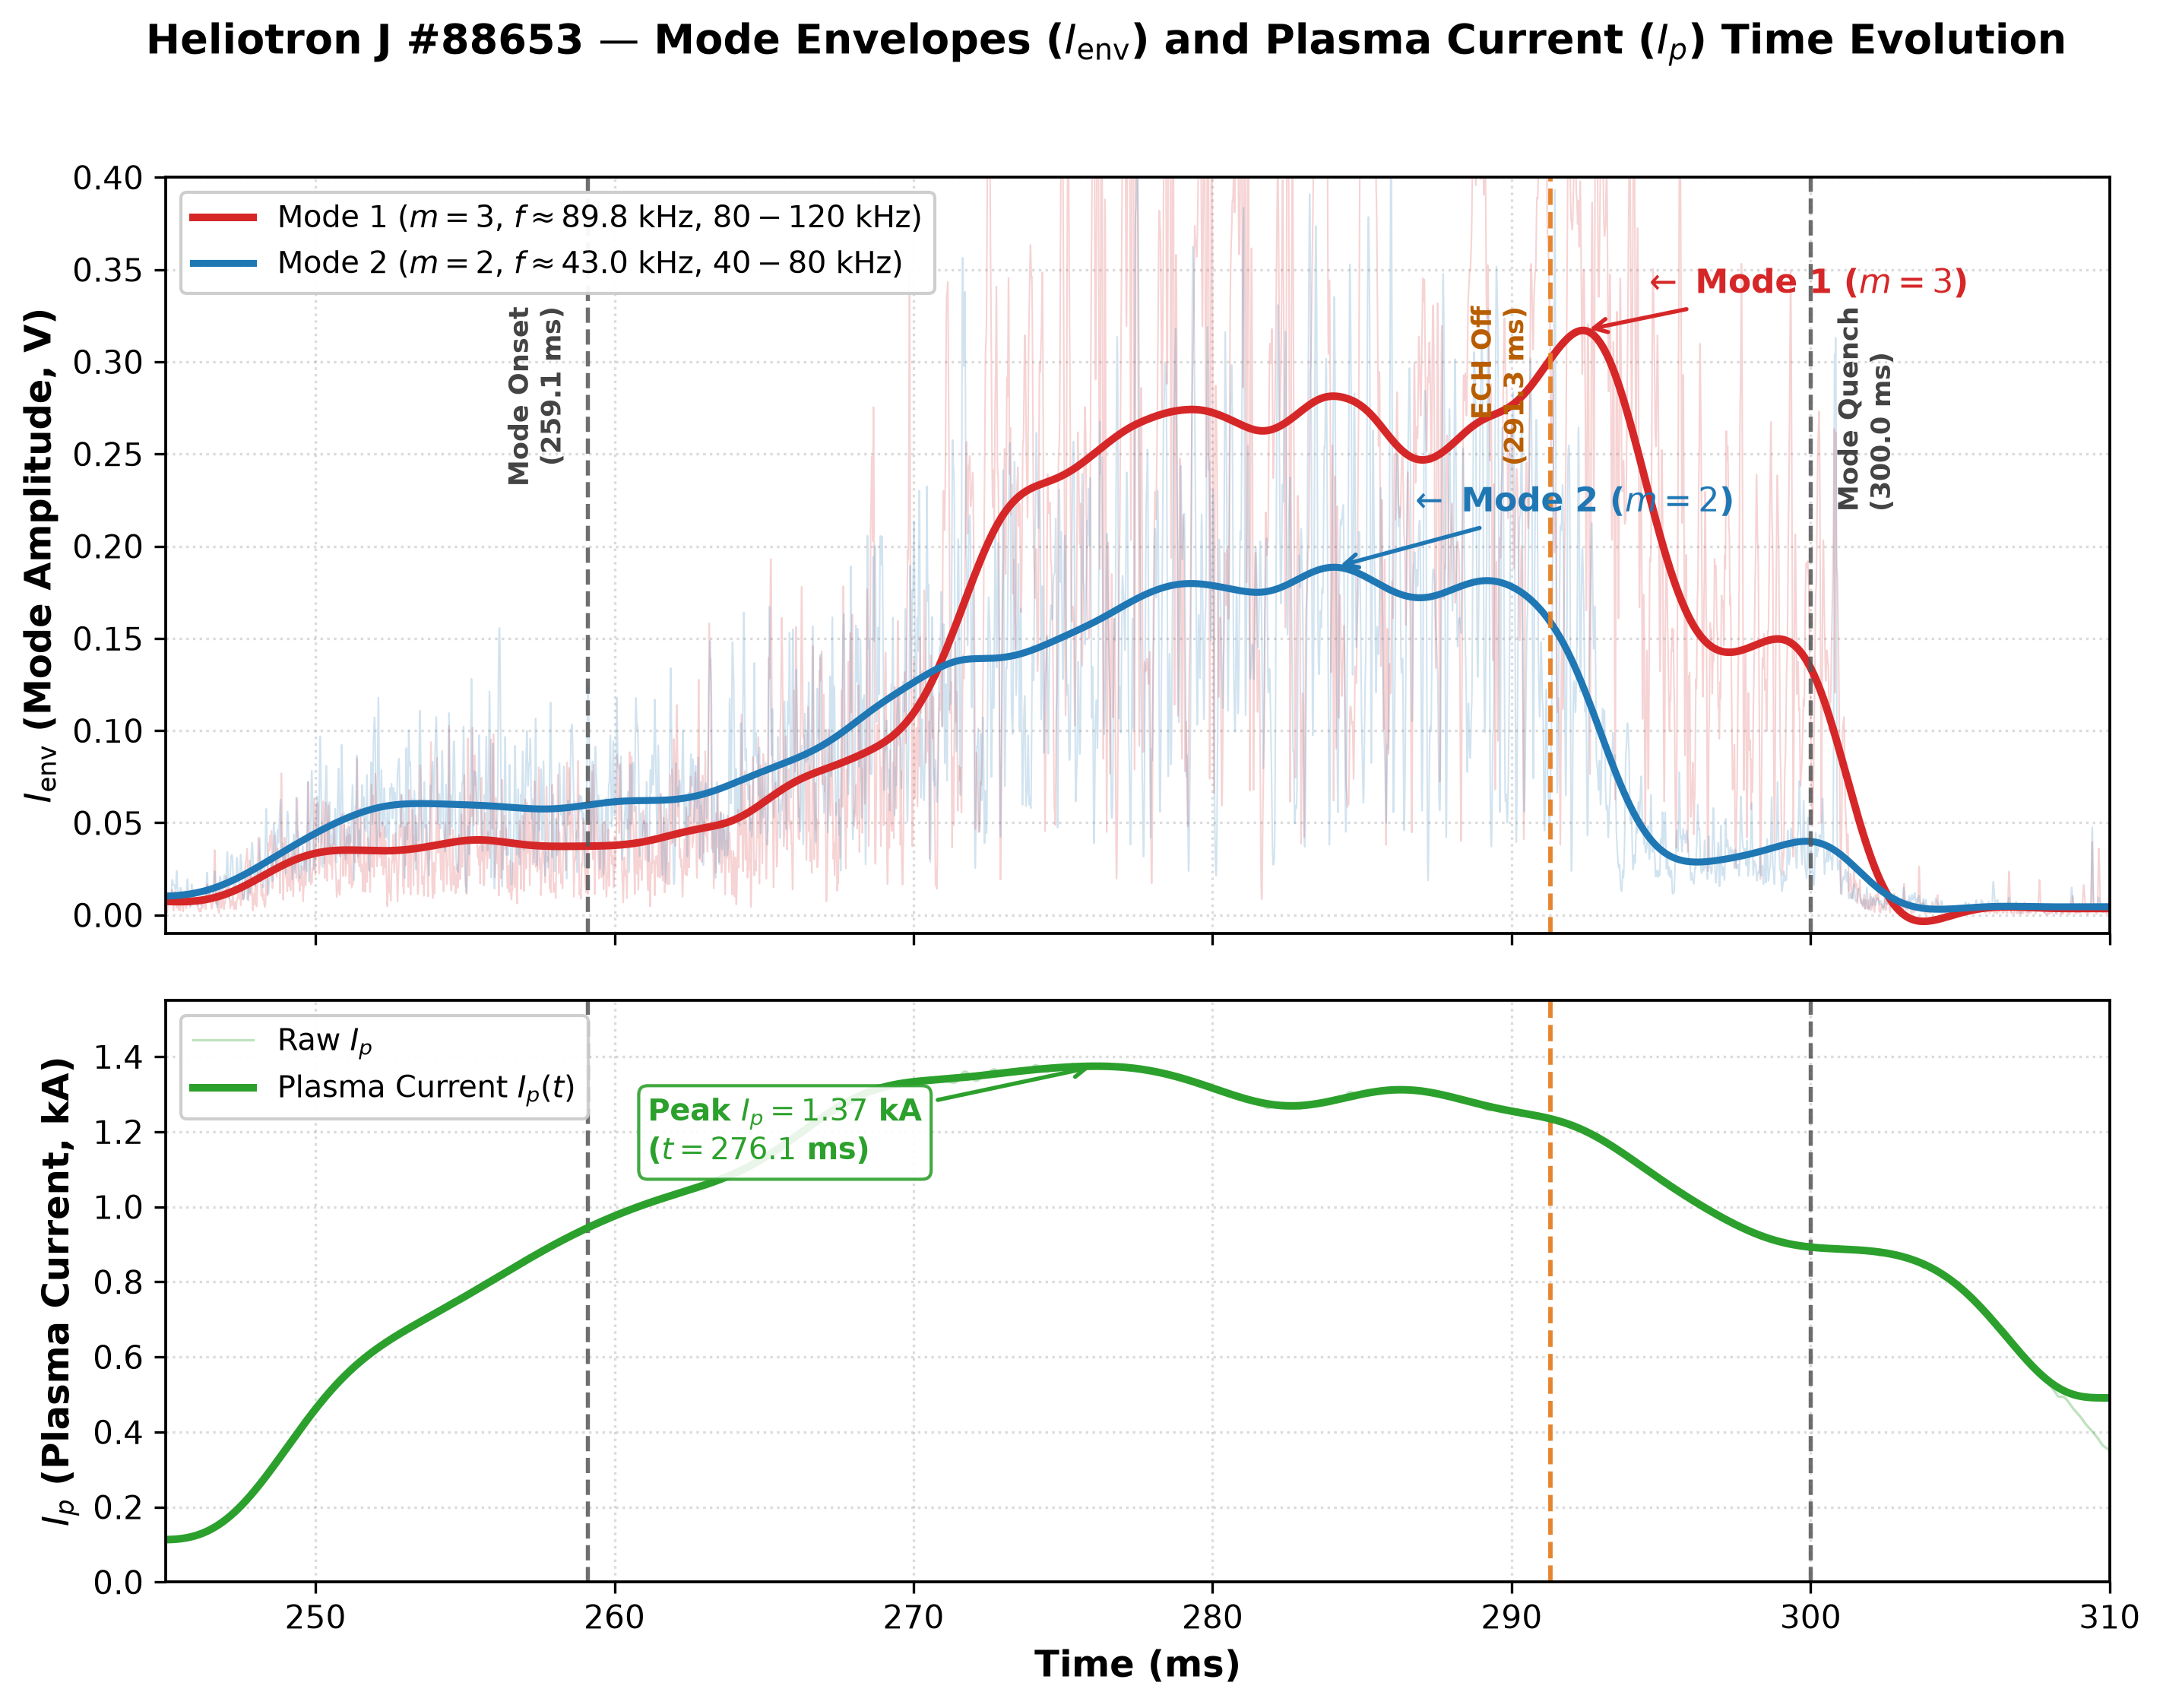
\includegraphics[height=0.75\textheight]{Images/obj2_dynamics_and_structure/mhd_mode_envelopes_and_ip_evolution_shot_88653.png}
    \end{figure}
    \tiny
    \textbf{Correction:} the ``Mode 2 quenches'' annotation on this figure is
    an artifact of the \emph{fixed} 40--80 kHz Bessel band losing the
    secondary mode as it downshifts to 35--40 kHz after ECH shut-off. An
    adaptive-band re-extraction (25--65 kHz) shows the envelope at
    $4.6\times$ the local noise floor at $t=295$--298 ms -- the mode
    downshifts, it does \emph{not} vanish. (Mode~2's $m=2$ is tentative, see the
    poloidal-number table.)
\end{frame}

\begin{frame}{Backup: Hysteresis Loop -- Plasma Current vs.\ Mode Envelope}
    \begin{figure}[h!]
        \centering
        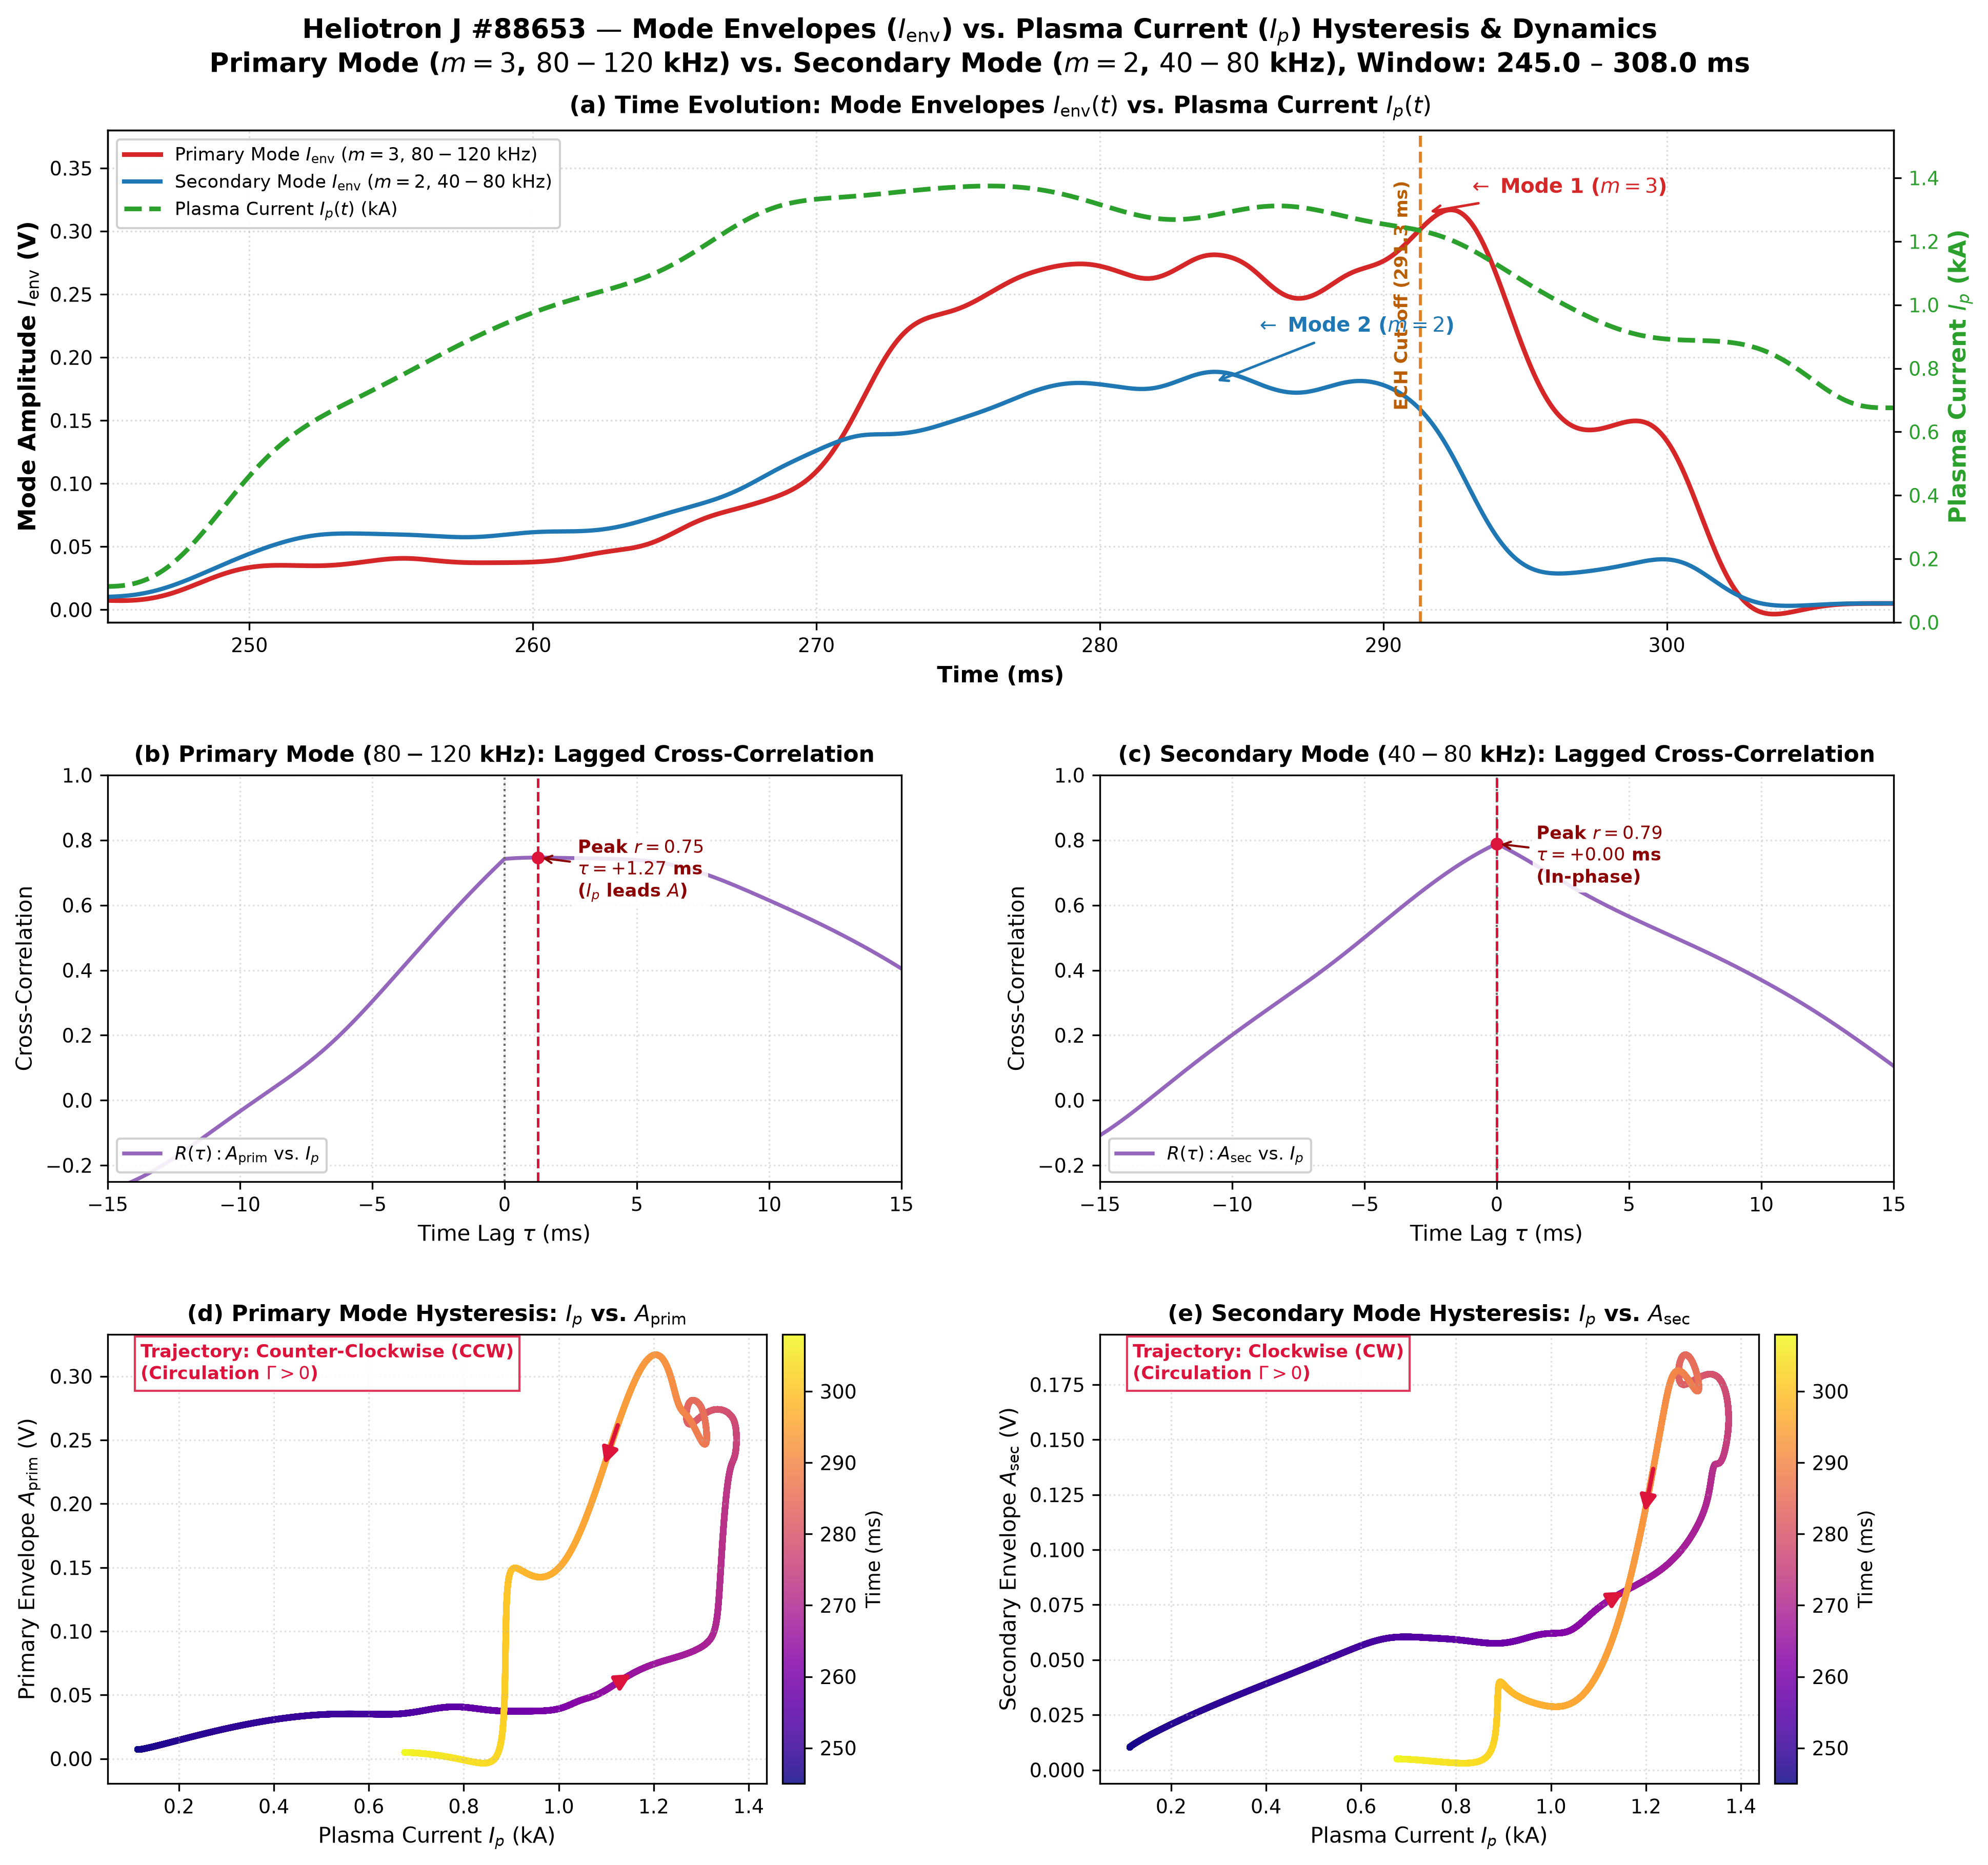
\includegraphics[height=0.75\textheight]{Images/obj2_dynamics_and_structure/mhd_hysteresis_ip_vs_envelope_dual_modes_shot_88653.png}
    \end{figure}
    \tiny
    \textbf{Same correction applies:} the apparent secondary-mode collapse
    in this hysteresis trace reflects the same fixed-band filter-edge
    effect, not a physical quench -- see the previous backup slide.
\end{frame}

\begin{frame}{Backup: Dual-Mode Envelope Coherence (Inter-Mode Modulation)}
    \begin{figure}[h!]
        \centering
        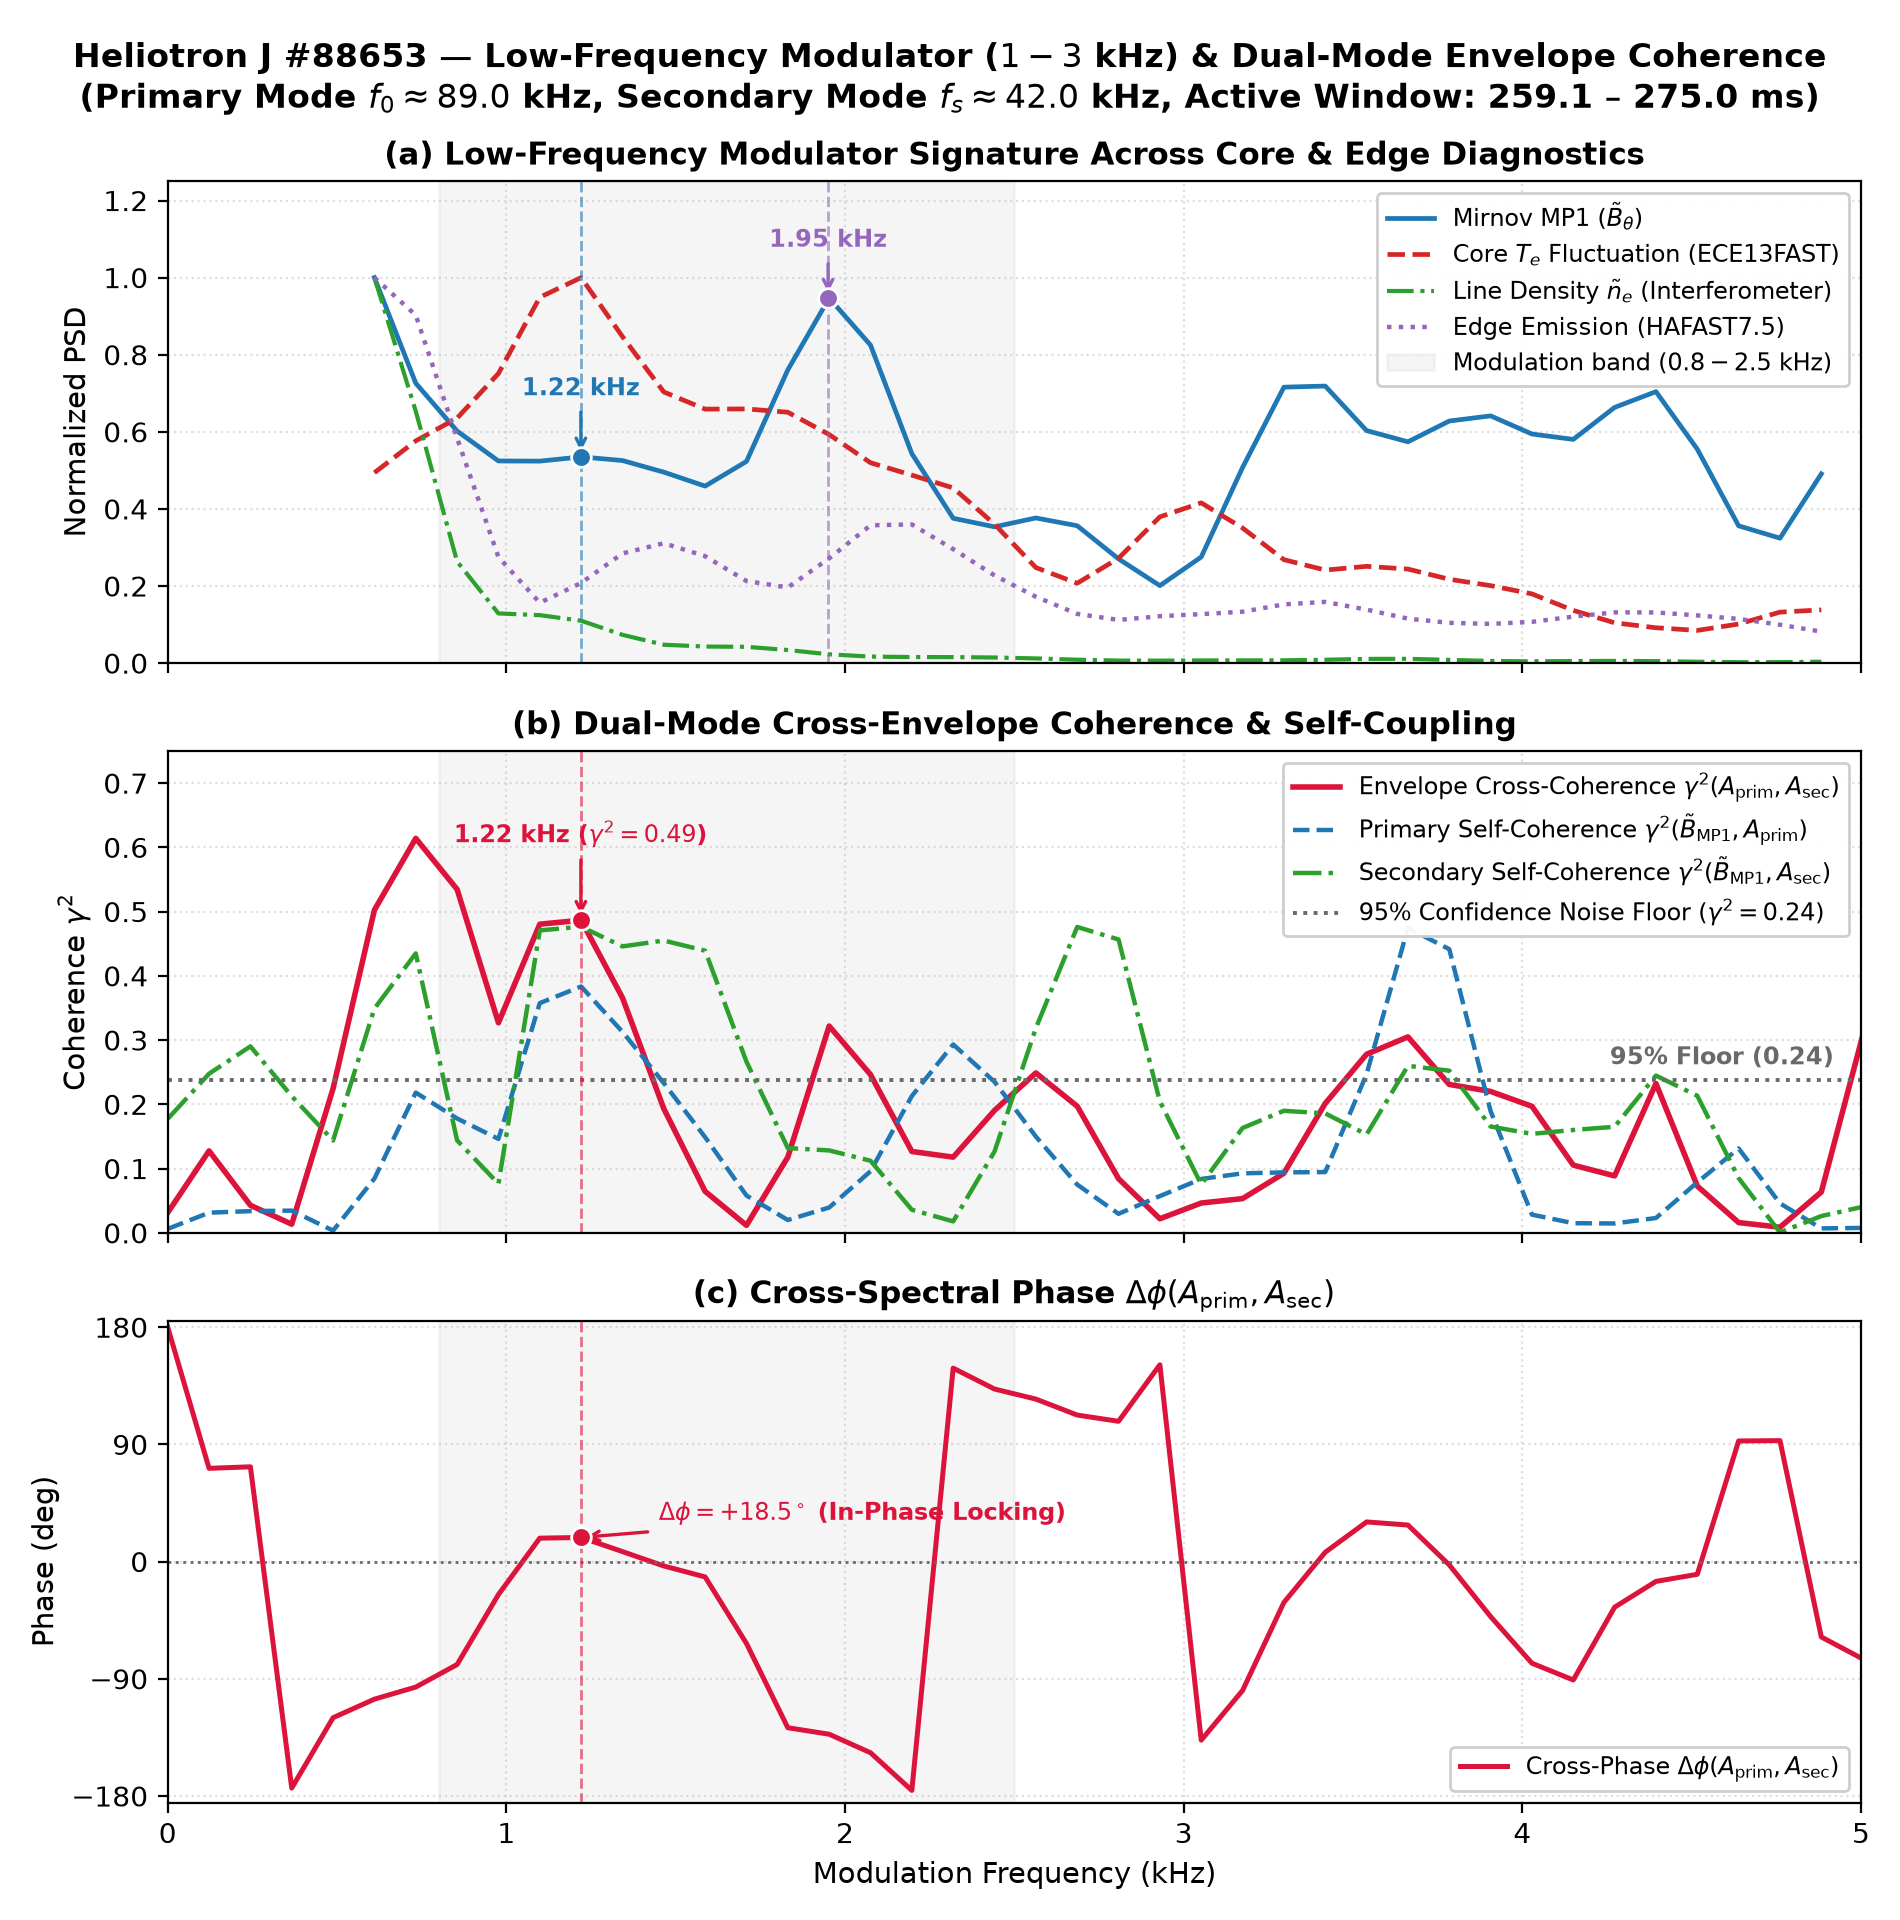
\includegraphics[height=0.85\textheight]{Images/obj2_dynamics_and_structure/mhd_modulator_dual_mode_coherence_shot_88653.png}
    \end{figure}
\end{frame}

\begin{frame}{Backup: Secondary--Primary Mode-Mixing Correlation}
    \begin{columns}[T]
        \begin{column}{0.5\textwidth}
            \centering Secondary branch ($\sim$\SI{43}{kHz})\\
            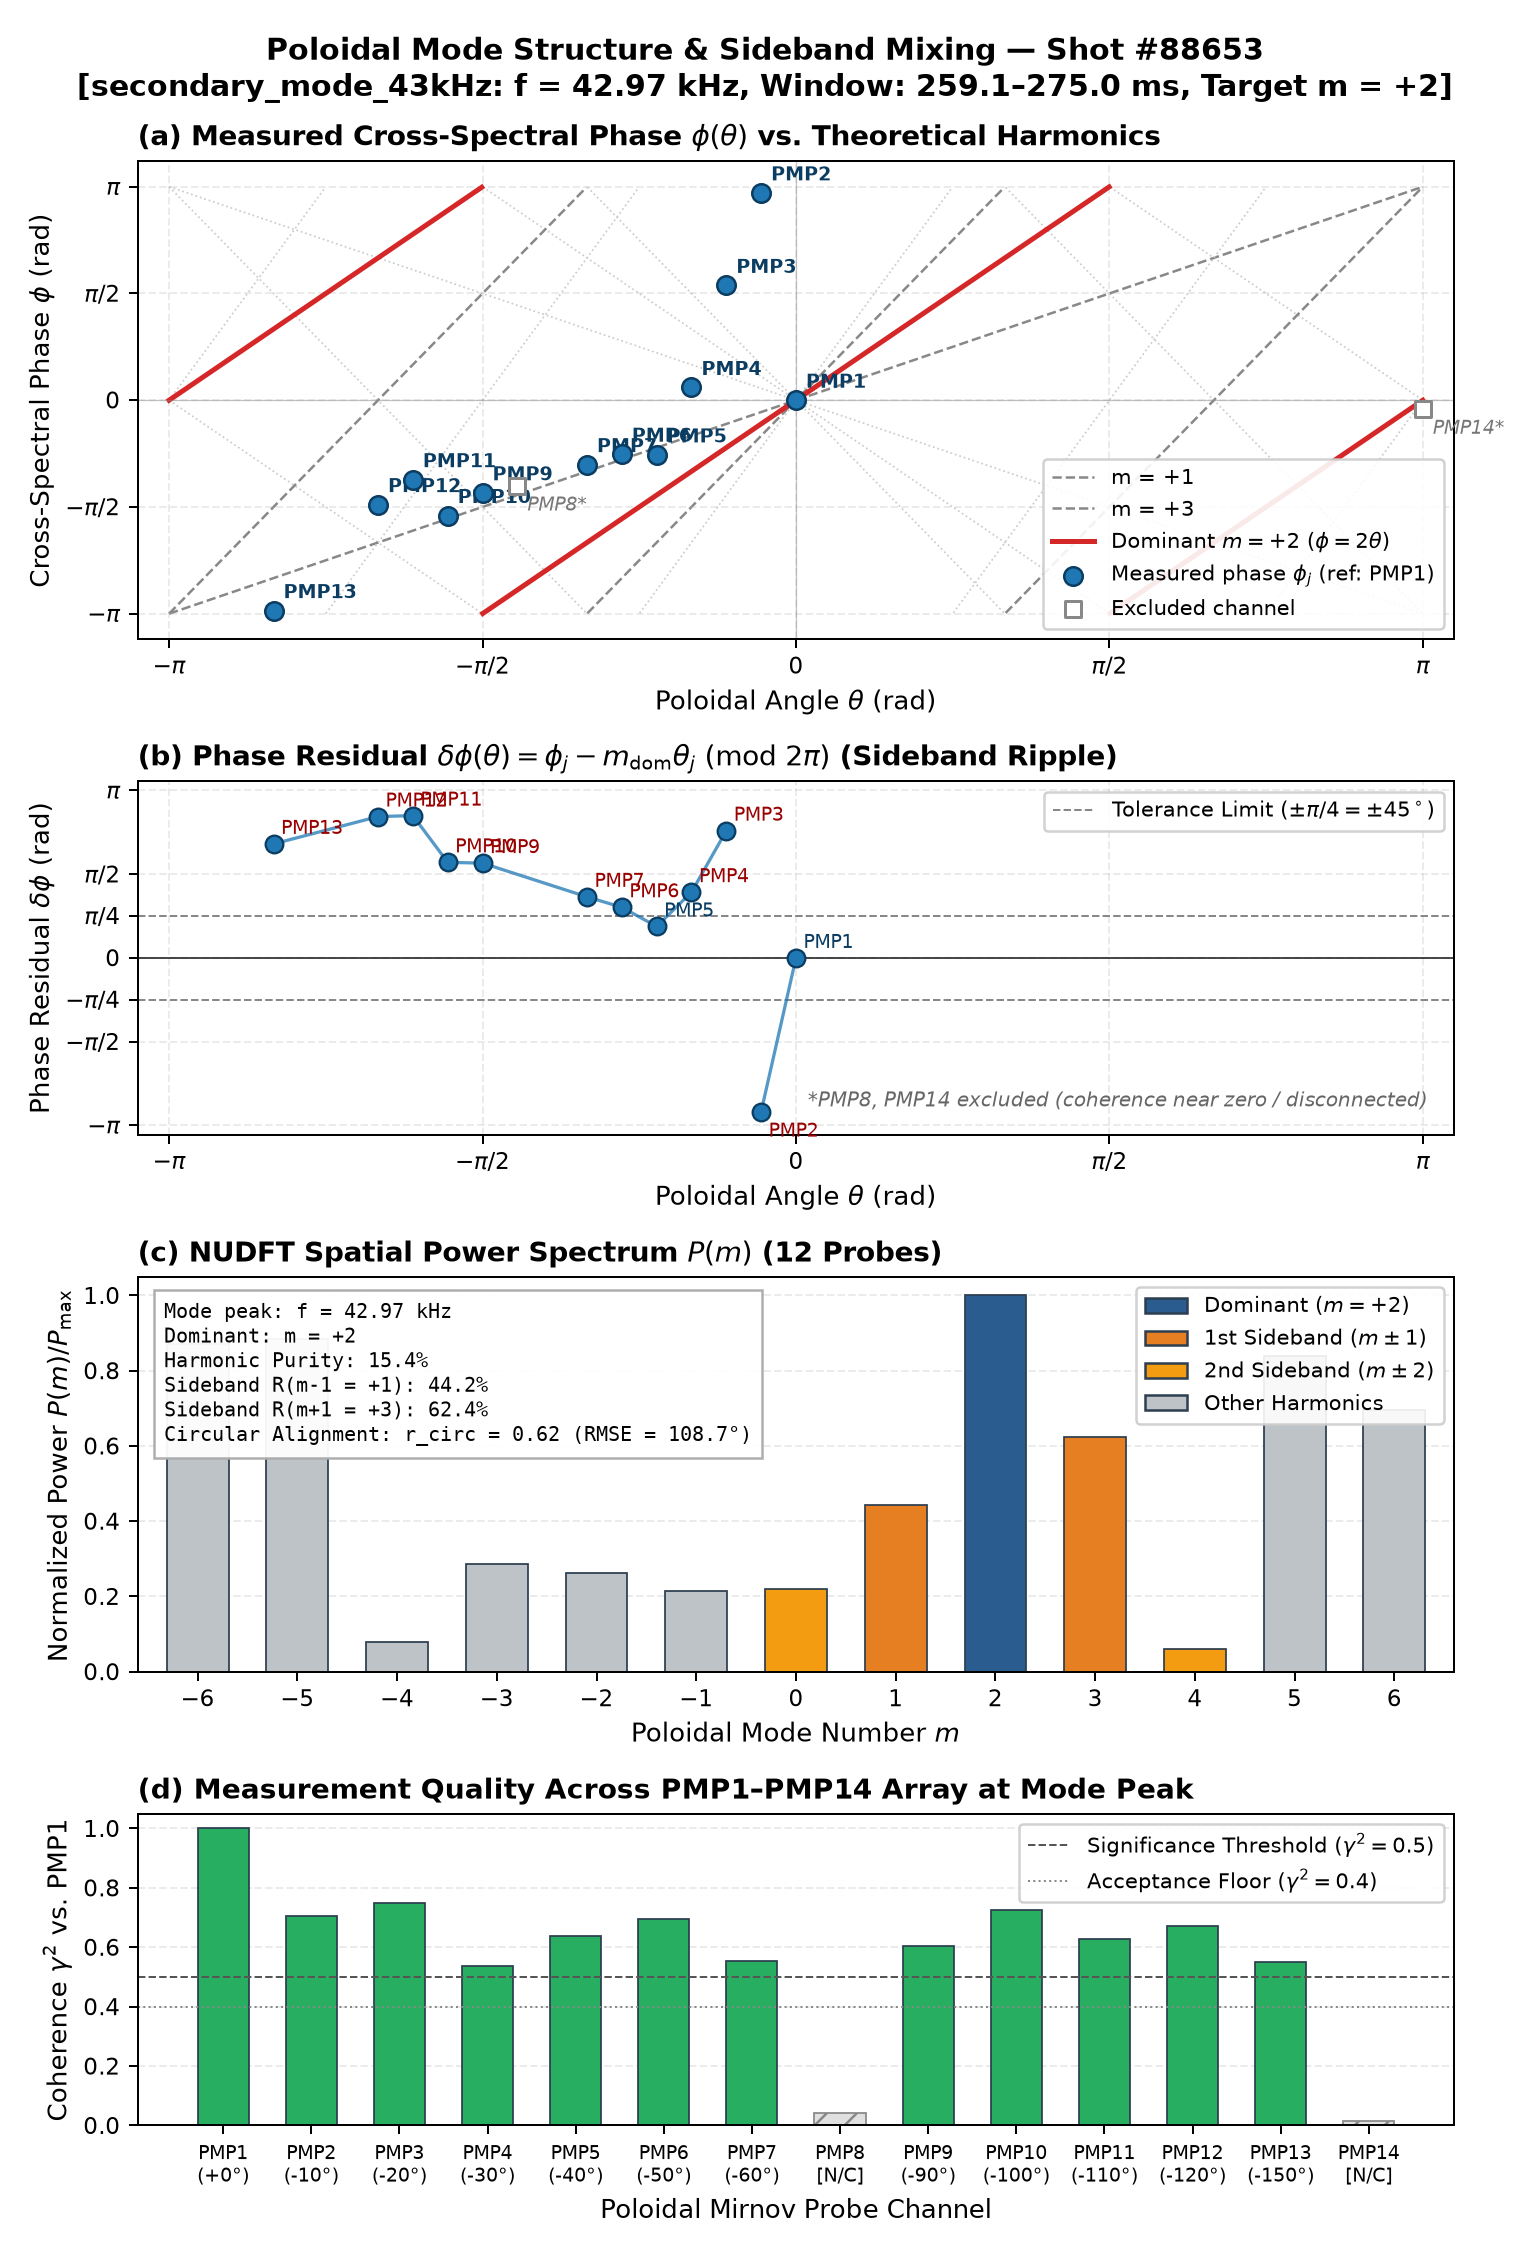
\includegraphics[width=0.62\textwidth]{Images/obj3_nonlinear_coupling/mhd_mode_mixing_shot_88653_secondary_mode_43kHz.png}
        \end{column}
        \begin{column}{0.5\textwidth}
            \centering Primary branch ($\sim$\SI{90}{kHz})\\
            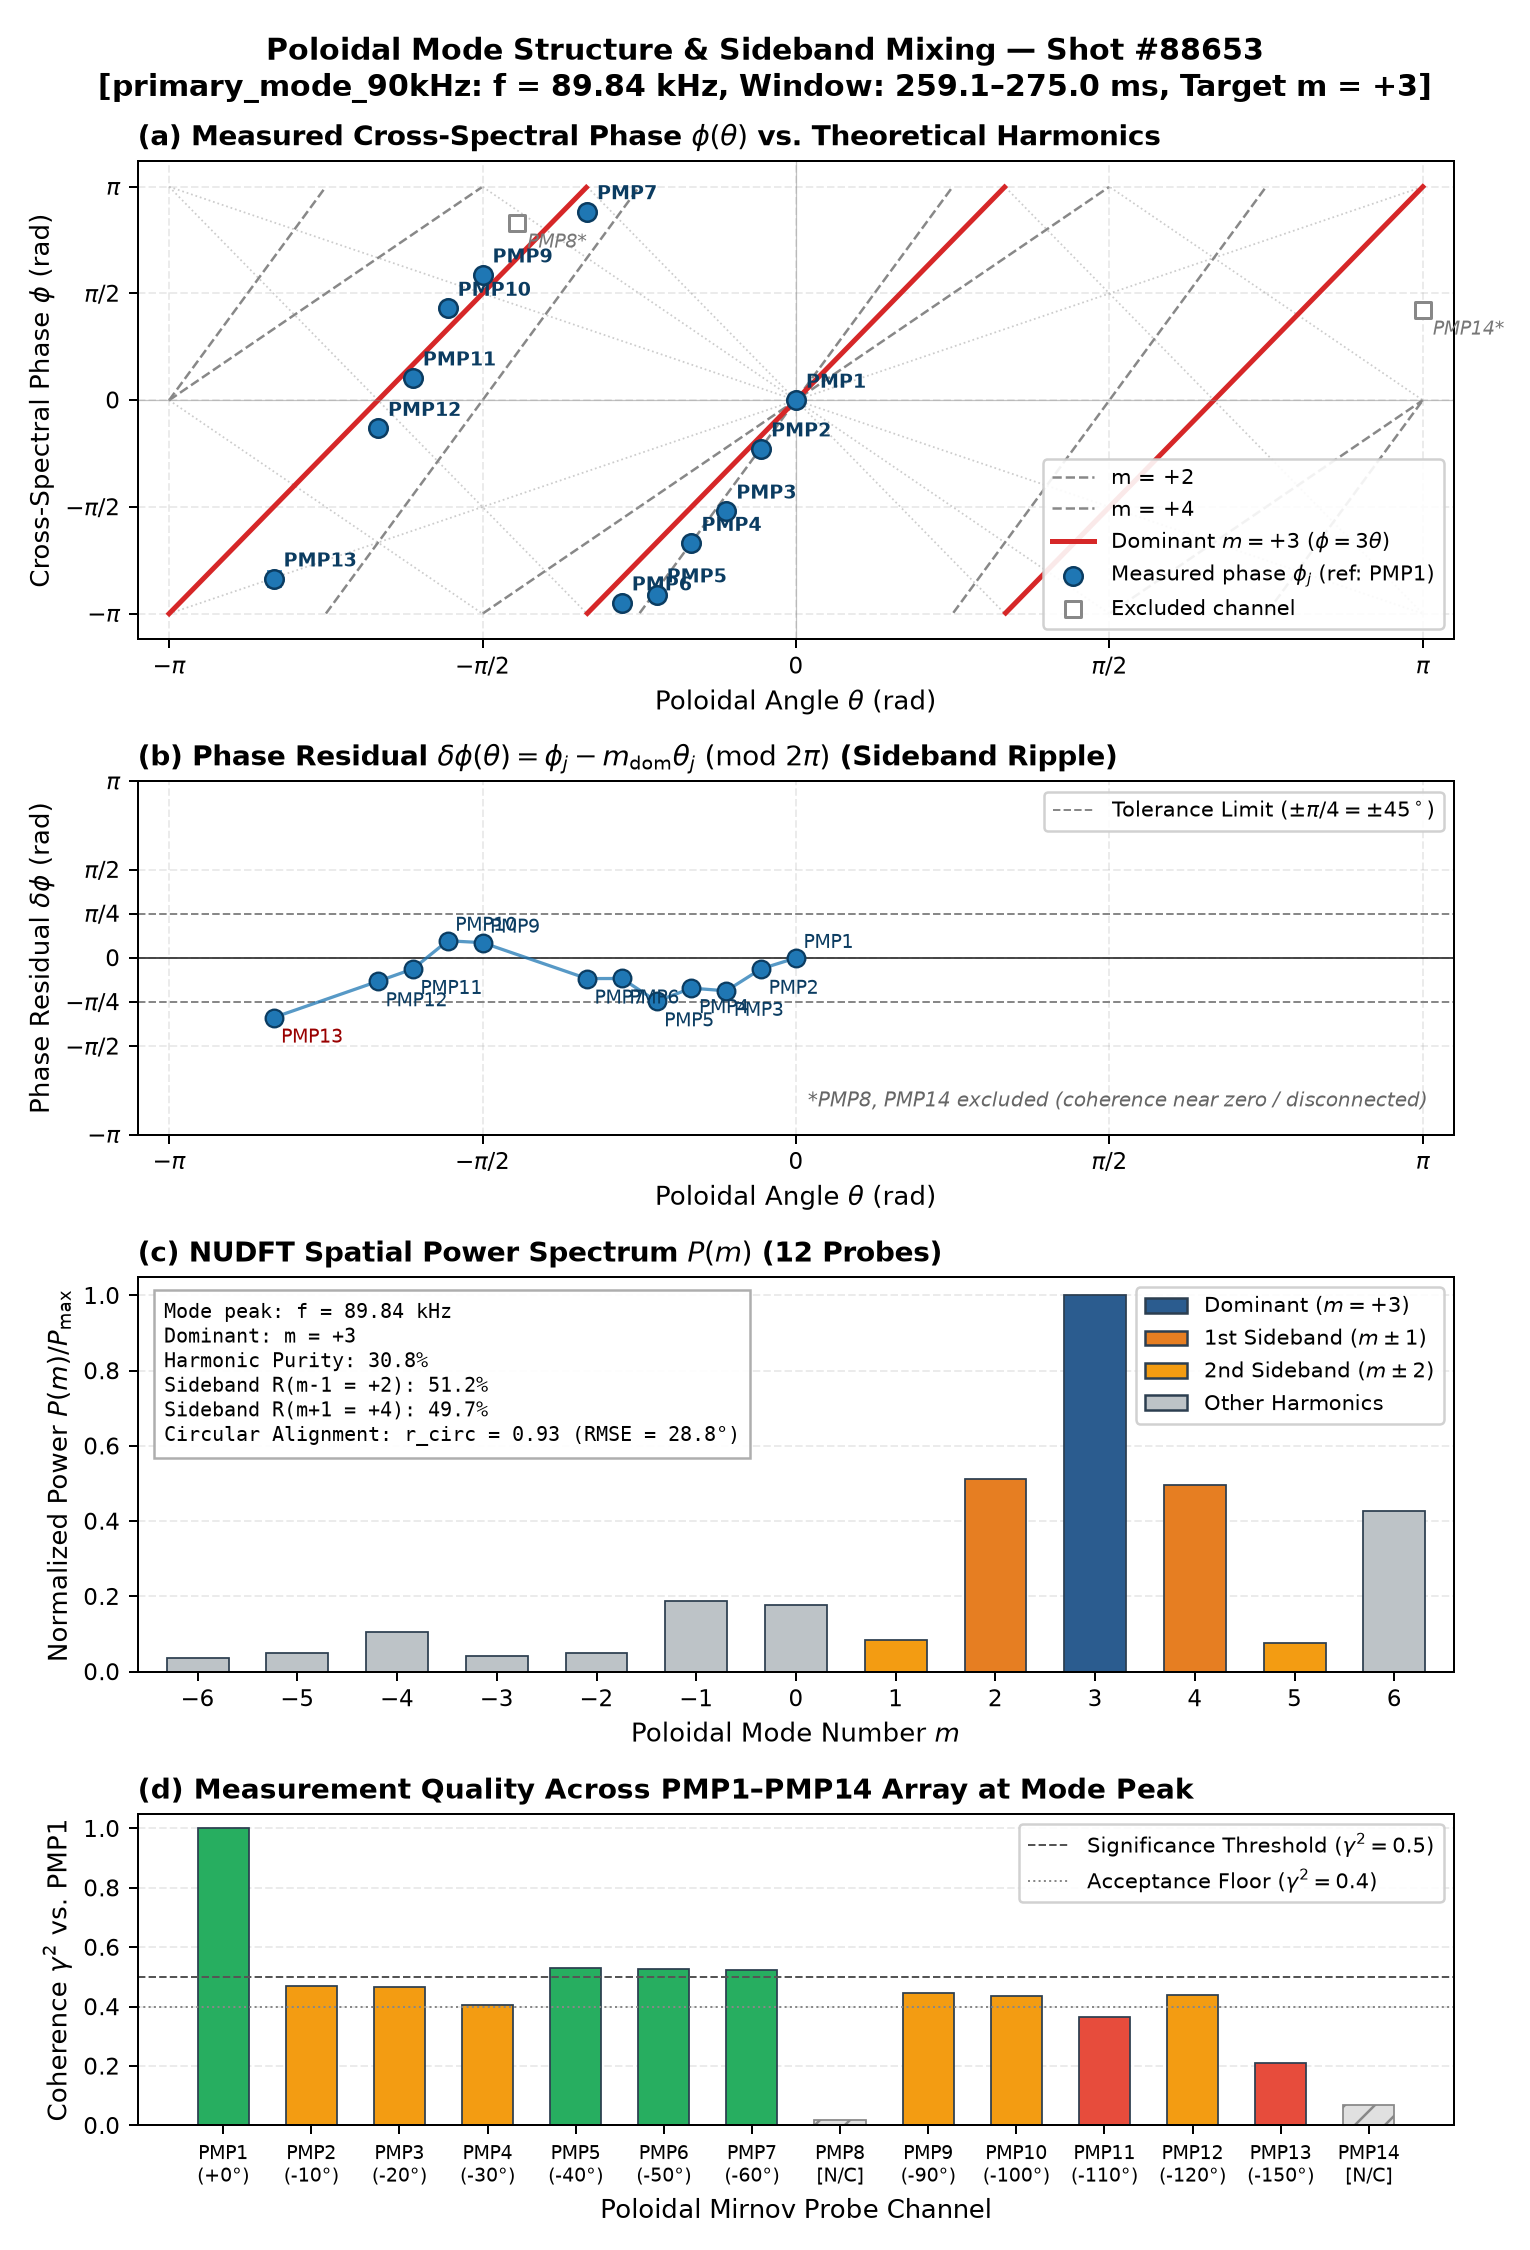
\includegraphics[width=0.62\textwidth]{Images/obj3_nonlinear_coupling/mhd_mode_mixing_shot_88653_primary_mode_90kHz.png}
        \end{column}
    \end{columns}
    \vspace{0.2cm}
    \tiny Additional correlation-metric view of inter-band mixing between the Secondary and Primary
    envelopes, complementing the dual-mode coherence above. Numbers on this slide have not
    been independently re-verified against the pipeline outputs in this round -- check
    against the underlying script before quoting specific values live.
\end{frame}

\begin{frame}{Backup: Carrier ($\tilde{B}$) vs.\ Envelope}
    \begin{figure}[h!]
        \centering
        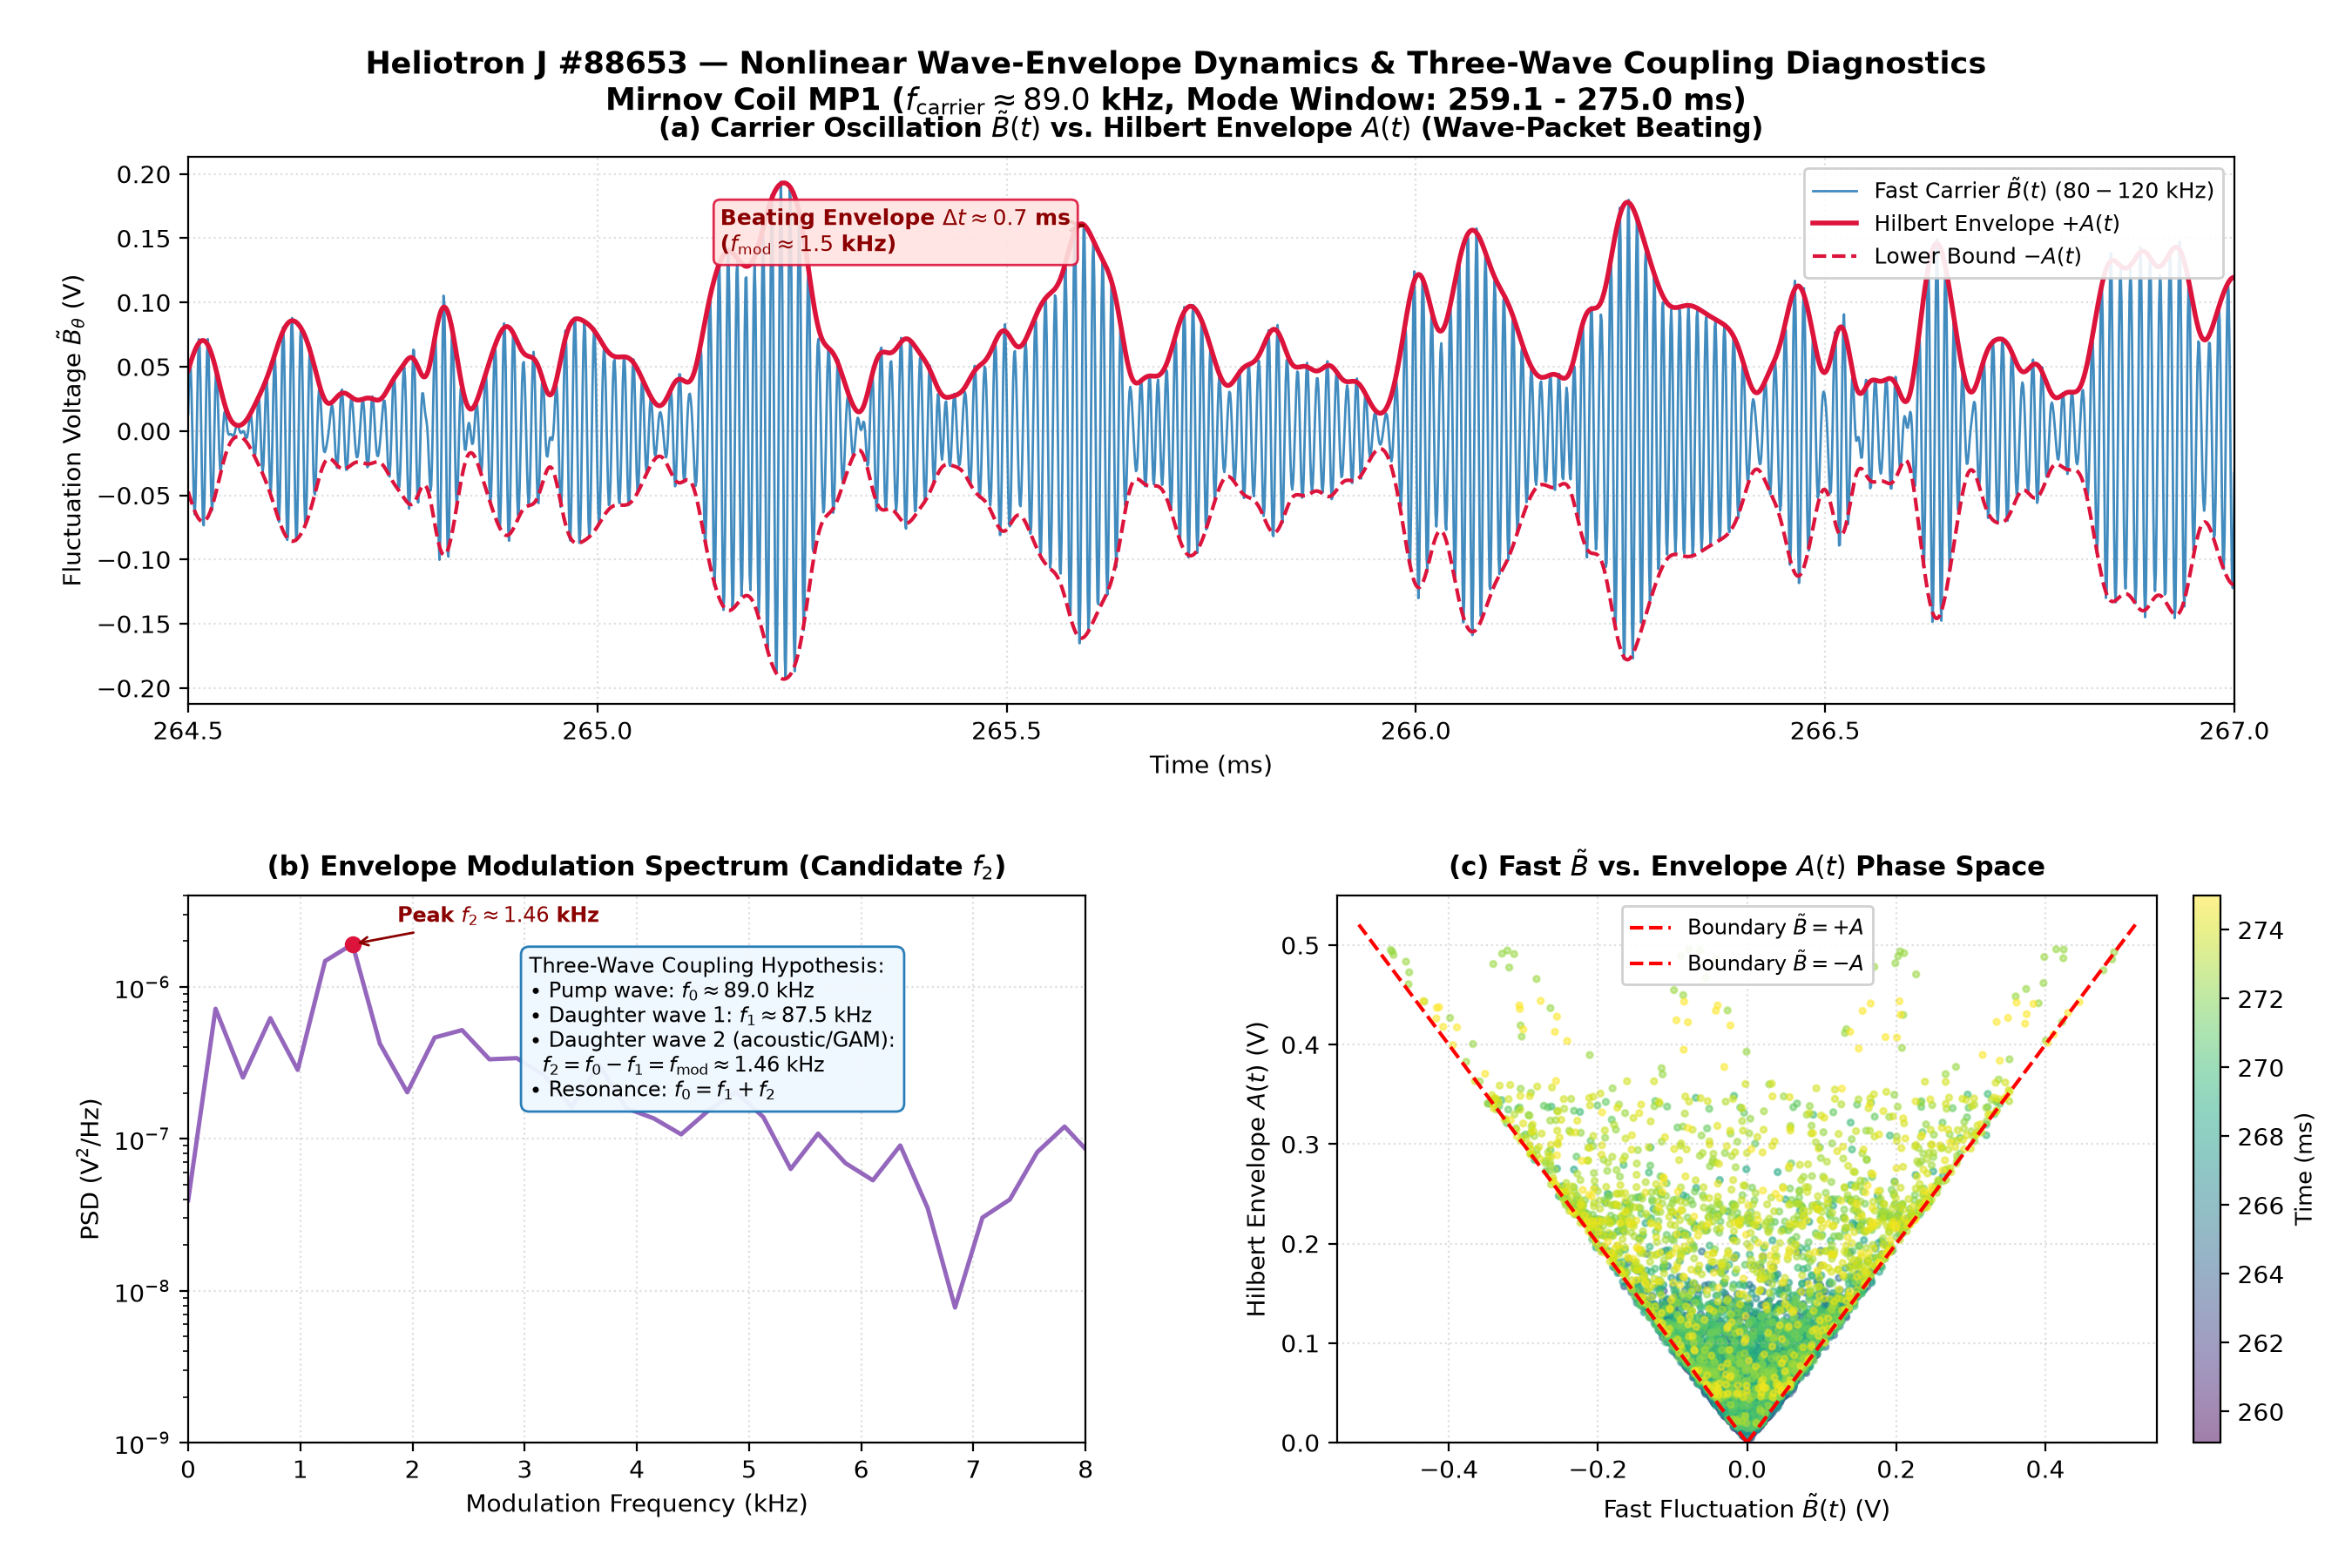
\includegraphics[height=0.85\textheight]{Images/obj2_dynamics_and_structure/mhd_b_tilde_vs_envelope_shot_88653.png}
    \end{figure}
\end{frame}

\begin{frame}{Backup: SNR vs.\ H$\alpha$ Emission Correlation}
    \begin{figure}[h!]
        \centering
        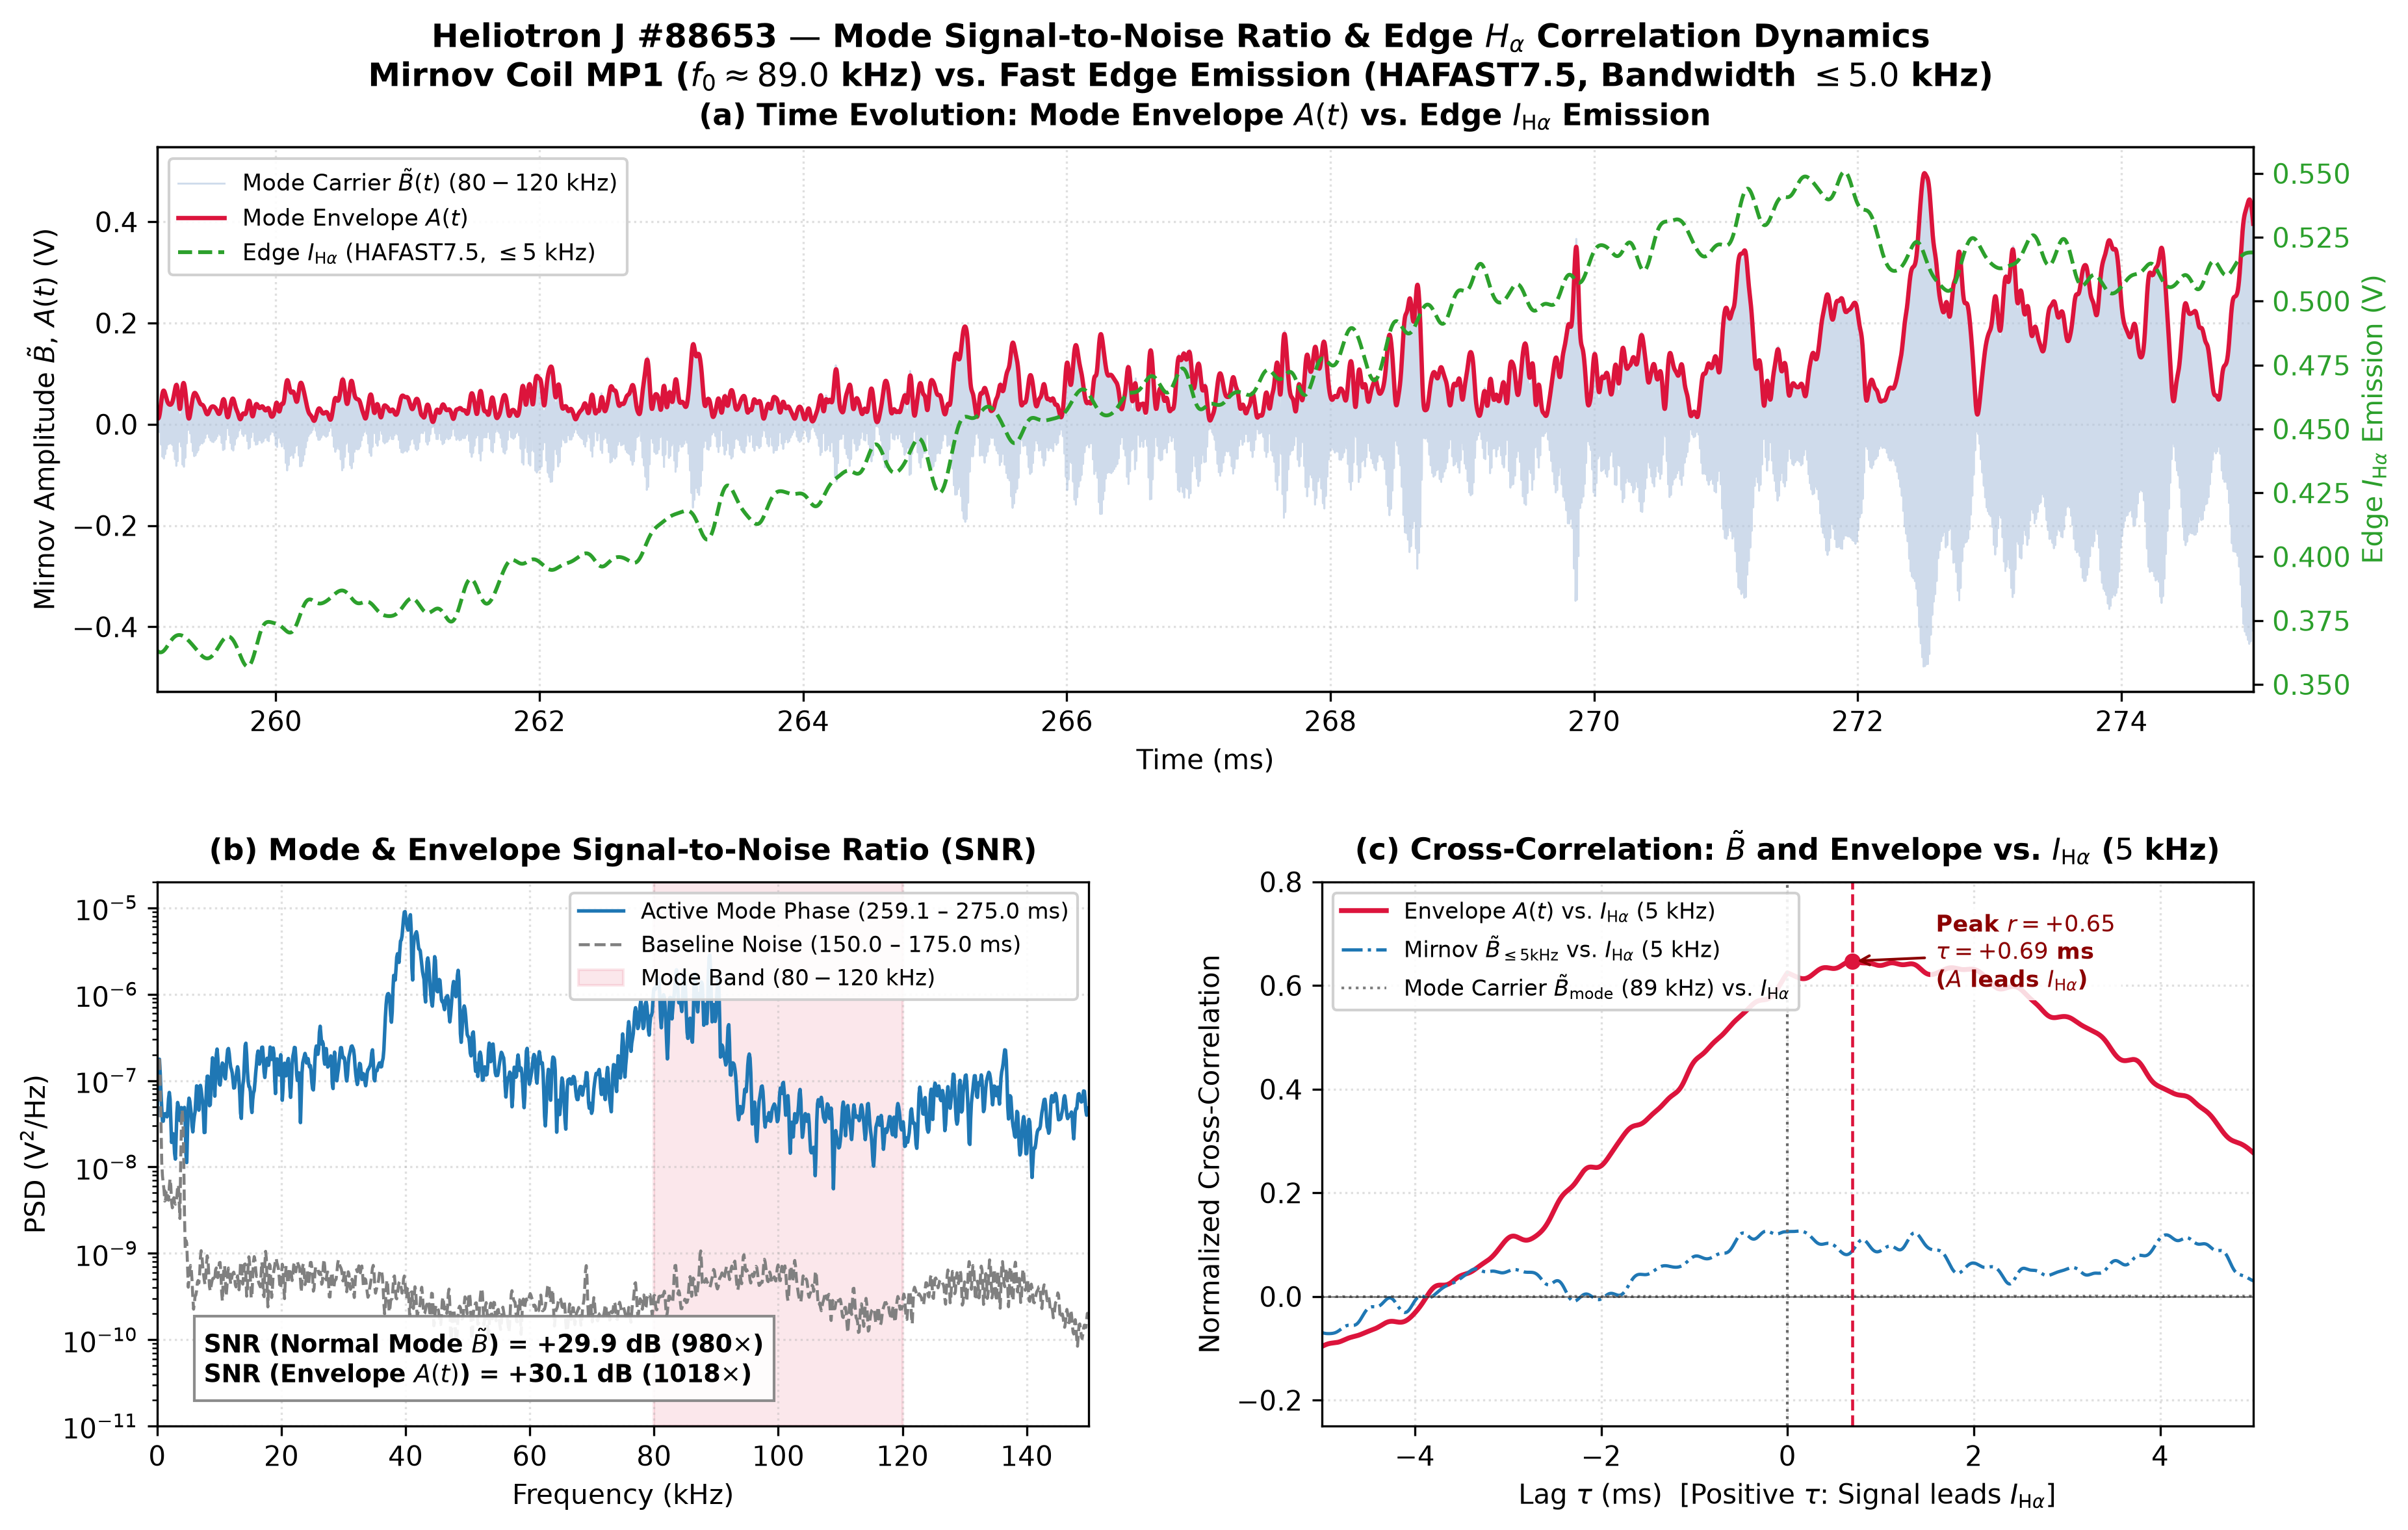
\includegraphics[height=0.85\textheight]{Images/obj2_dynamics_and_structure/mhd_snr_halpha_correlation_shot_88653.png}
    \end{figure}
\end{frame}

\subsection{Backup: Objective 3}

\begin{frame}{Backup: Objective 3 -- Four Candidate Mechanisms (Detailed)}
    \scriptsize
    \renewcommand{\arraystretch}{1.15}
    \setlength{\tabcolsep}{4pt}
    \begin{tabularx}{\textwidth}{@{}p{3.0cm}p{2.6cm}X@{}}
        \toprule
        \textbf{Mechanism} & \textbf{Plausibility} & \textbf{Why} \\
        \midrule
        \textbf{Harmonic self-coupling} & 
        \textcolor{orange!70!black}{\textbf{Plausible / unconfirmed}} &
        The $\sim$\SI{50}{kHz} line generating its own second harmonic
        ($50+50\to100$\,kHz, upward flow); no second wave required. Scaling is
        inconclusive and the band-peak ratio (2.2--2.6) disfavors an exact 1:2 pair. \\
        \addlinespace
        Degenerate parametric decay (PDI) &
        \textcolor{orange!80!black}{\textbf{Low / unconfirmed}} &
        Decay would give $\mathrm{Im}[B_{\text{sum}}]<0$; the 16 highest-SNR
        windows are $>0$. Candidate ``pump'' (\SI{98.6}{kHz}) is $\sim$10\% off
        the validated primary mode; no independent second wave found; fails
        double-validation. \\
        \addlinespace
        Period-doubling bifurcation &
        \textcolor{orange!80!black}{\textbf{Unconfirmed / open}} &
        No amplitude-threshold signature or subharmonic cascade ($f_1/4$, etc.)
        is observed. \\
        \addlinespace
        EPM/BAE sidebands (Berk--Breizman) &
        \textcolor{green!50!black}{\textbf{Real, different feature}} &
        Explains the multi-branch frequency hopping well, but such sidebands
        are not normally locked to an exact 1:2 ratio. \\
        \bottomrule
    \end{tabularx}
    \vspace{0.2cm}
    \normalsize
    Note: the amplitude-scaling analysis (main deck, Slide~12) yields
    pooled scaling ($2.10{-}2.26$), but within-episode slopes near $1.0$ and peak
    frequency ratios (${\sim}2.25$, tracking the independently validated 89-95 kHz mode) 
    make the mode origin inconclusive. Upward flow is observed in the highest-SNR windows (threshold-dependent); harmonic generation is neither confirmed nor excluded.
\end{frame}

\begin{frame}{Backup: All-window fit (slope 0.81) vs. high-SNR windows}
    \begin{figure}
        \centering
        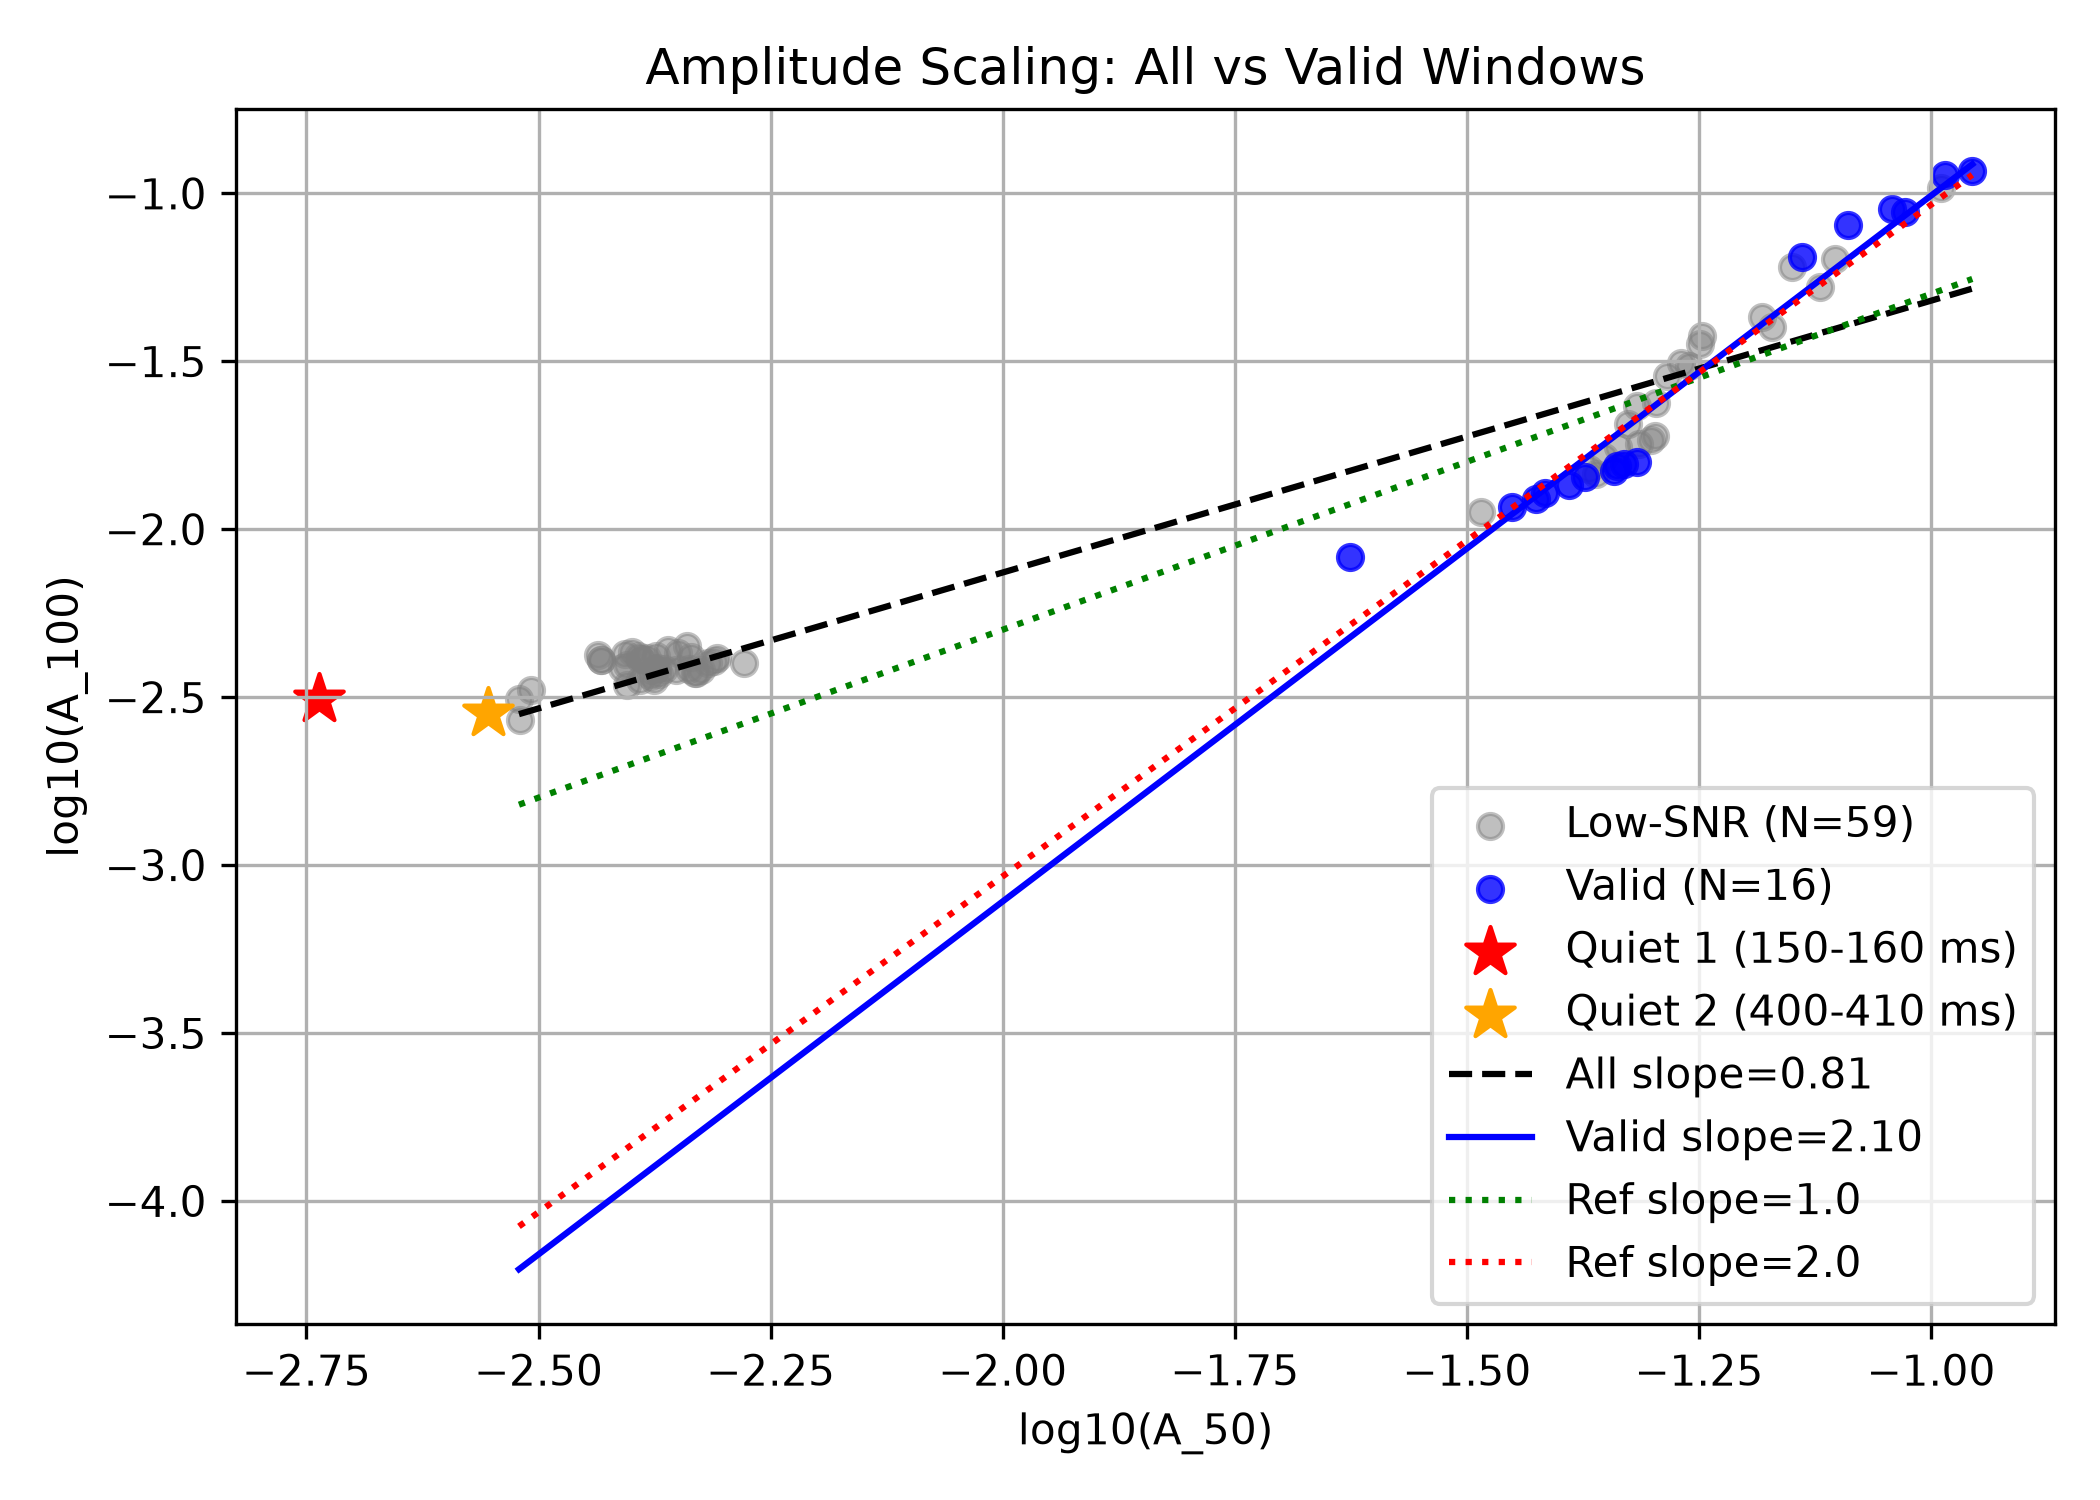
\includegraphics[height=0.5\textheight]{Images/amplitude_scaling_all_vs_valid.png}
    \end{figure}
    \vspace{-0.2cm}
    \begin{itemize}
        \item Across all 75 sliding windows, the OLS slope drops to $0.81$.
        \item Grey low-SNR windows sit near the quiet-interval levels (stars); minimum plasma-phase band power (${\sim}10^{-5}$ $V^2$, incl.\ df) is comparable to quiet intervals -- consistent with a measurement noise limit (cause not proven).
    \end{itemize}
\end{frame}

\begin{frame}{Backup: Sign of Im[$B_{\text{sum}}$] vs SNR threshold}
    \begin{figure}[h!]
        \centering
        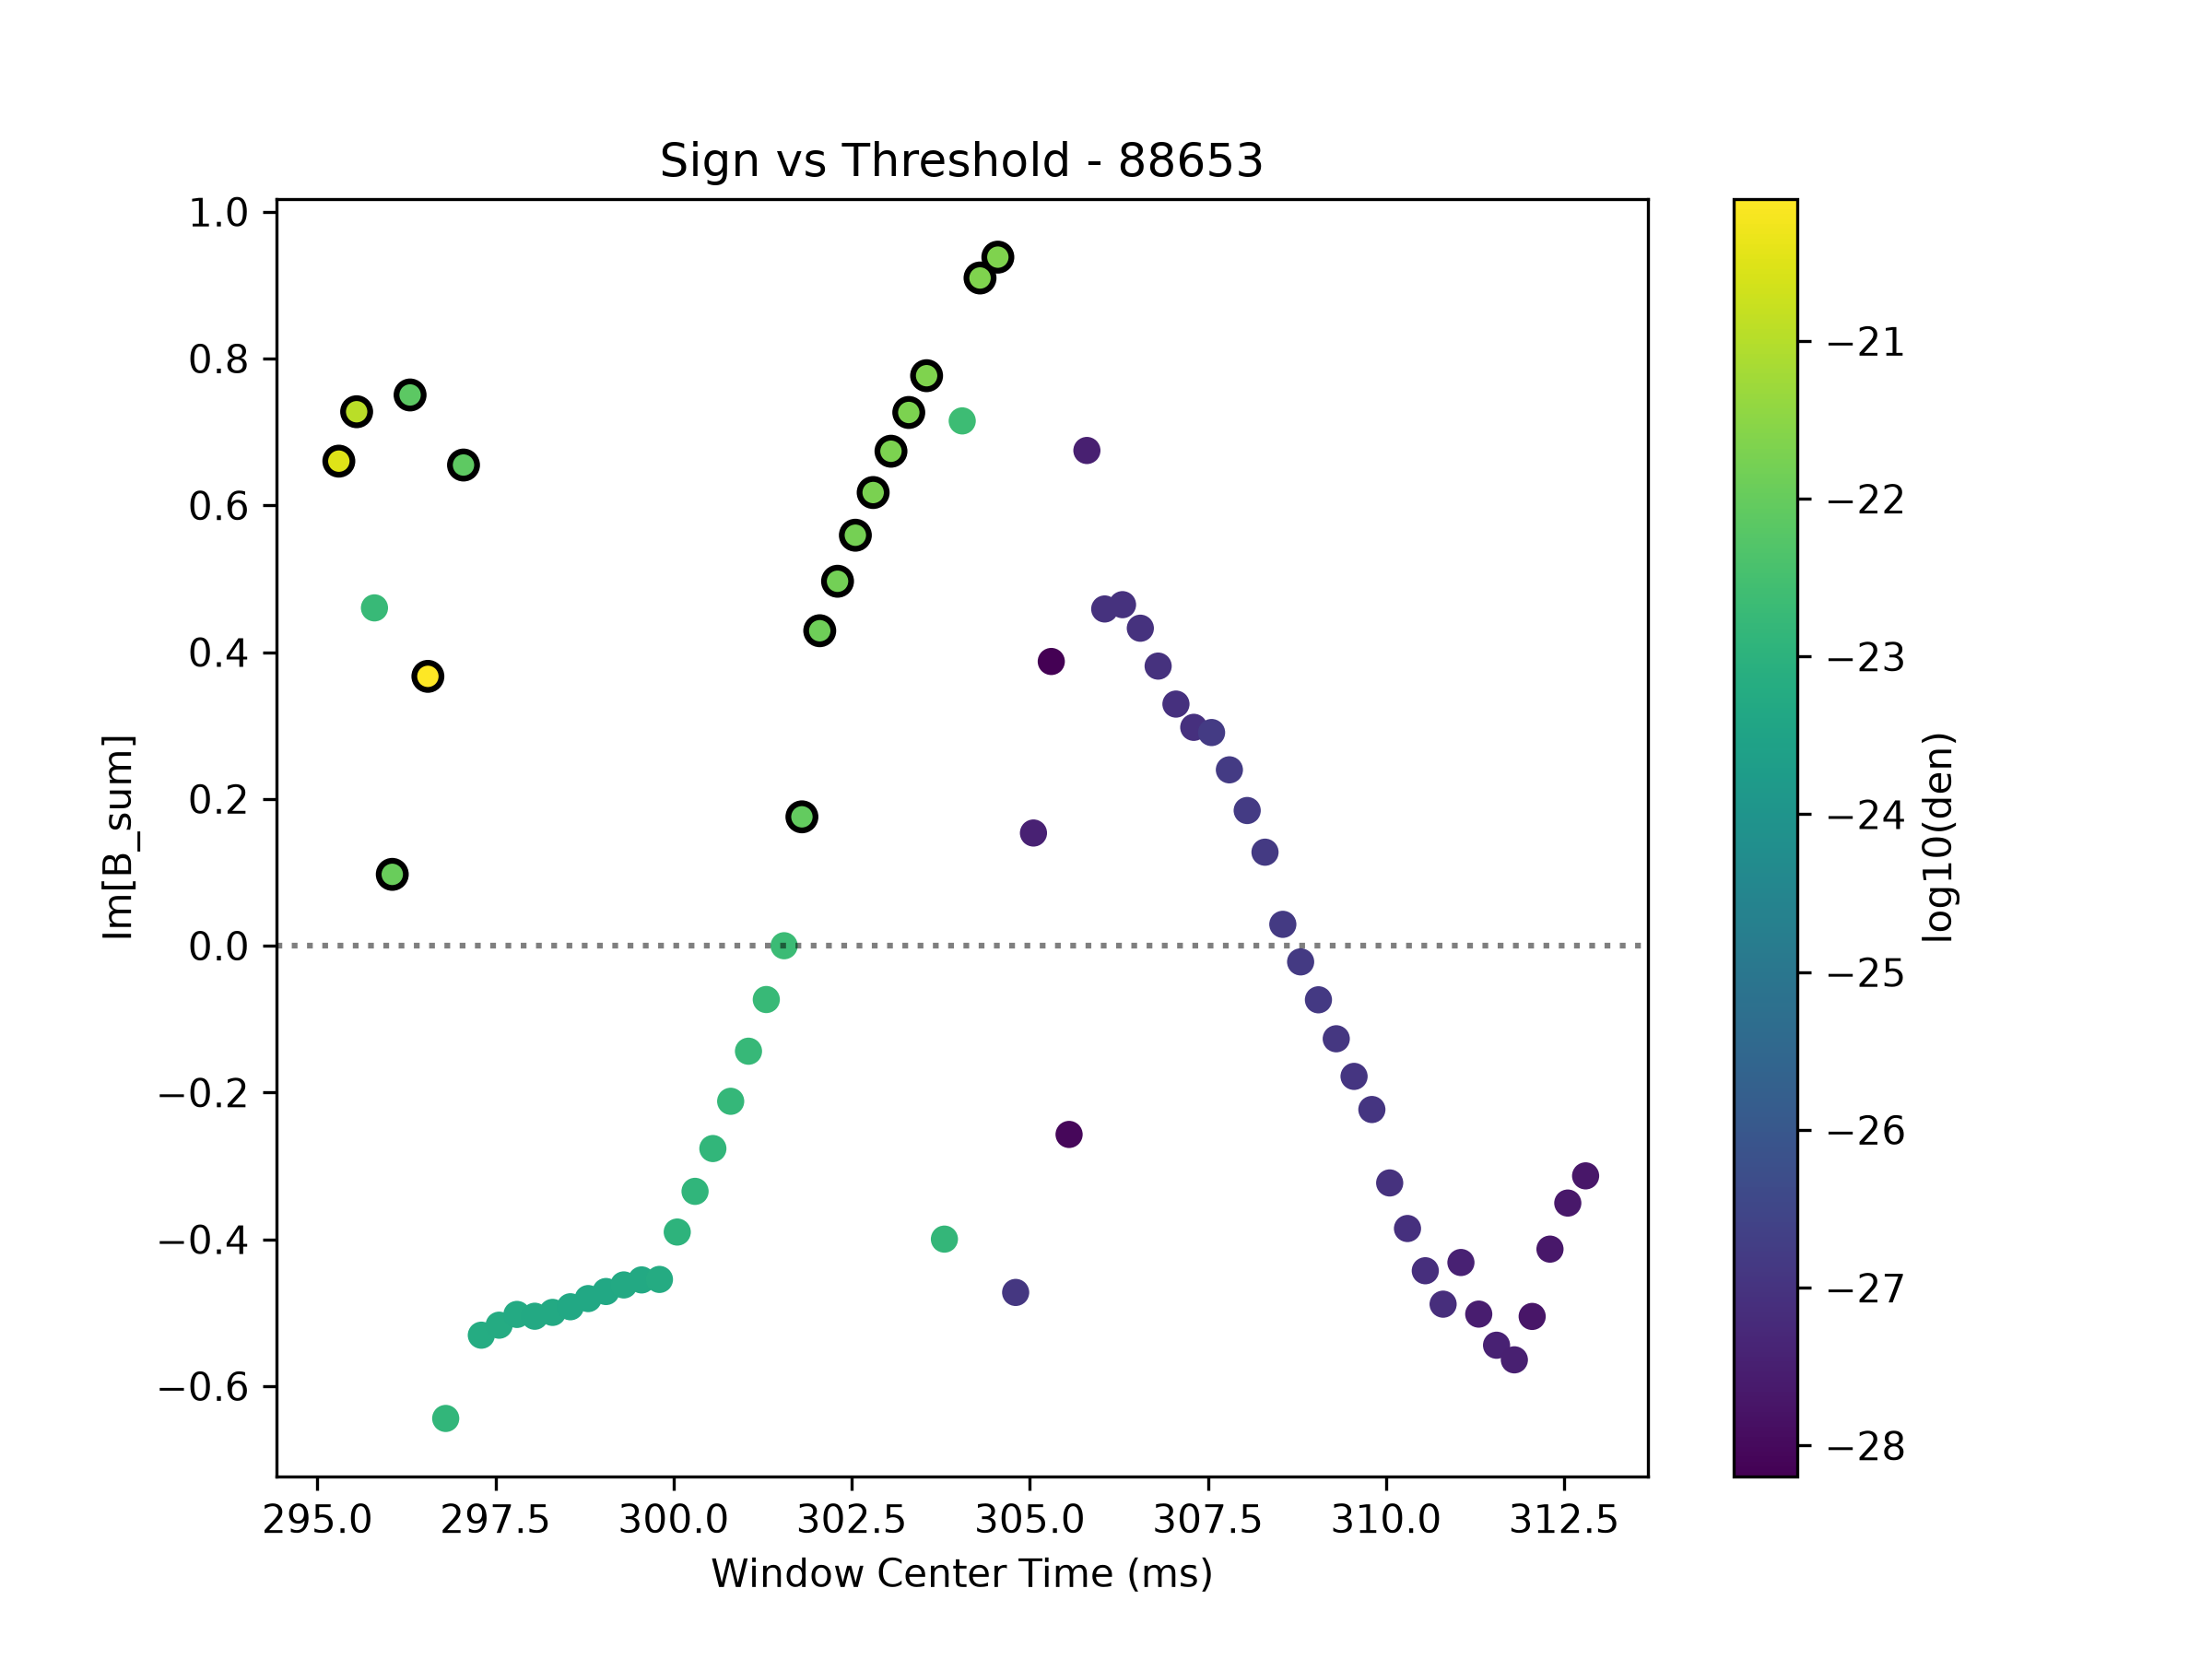
\includegraphics[height=0.5\textheight]{Images/sign_vs_threshold_88653.png}
        \\[-0.1cm]{\tiny Black edge: $\mathrm{den}>2.5\times10^{-23}$ (16 windows); colour = $\log_{10}(\mathrm{den})$.}
    \end{figure}
    
    \vspace{-0.2cm}
    \centering
    \footnotesize
    \begin{tabular}{ccc}
        \toprule
        \texttt{den} Threshold & Number of Windows & Positive Sign \\
        \midrule
        $2.5 - 4.0 \times 10^{-23}$ & 16 & 16 \\
        $2.0 \times 10^{-23}$ & 18 & 17 \\
        $1.5 \times 10^{-23}$ & 22 & 18 \\
        \bottomrule
    \end{tabular}
    
    \vspace{0.2cm}
    \begin{itemize}
        \item Just below the cut the biphase passes through zero near \SI{301.5}{ms}; the sign is threshold-dependent.
    \end{itemize}
\end{frame}

\begin{frame}{Backup: Objective 3 -- Total (Integrated) Bicoherence}
    \footnotesize
    $b^2_{\text{total}}(\text{band}) = \sum_{(f_1,f_2)\in\text{band}} b^2(f_1,f_2)$,
    dimensionless. Expected noise floor: $\mathbb{E}[b^2_{\text{total,noise}}]
    = N_{\text{bins}}/N_{\text{eff}}$ ($N_{\text{fft}}=512$,
    $f_s=\SI{1.0}{MHz}$, $\Delta f\approx\SI{1.95}{kHz}$; subharmonic band
    \SIrange{40}{80}{kHz} has $N_{\text{bins}}=4{,}800$).
    \vspace{0.15cm}
    \small
    \centering
        \begin{tabular}{lccc}
        \toprule
        Window ($N_{\text{eff}}{=}N_{\text{seg}}/2$) & Measured $b^2_{\text{total}}$ & Noise Floor & Ratio \\
        \midrule
        ECH+NBI (first 30 segments, \SIrange{259.1}{267.1}{ms}) & 168.85 & 320.0 & $0.53\times$ \\
        NBI-only (30 segments, \SIrange{291.3}{300.0}{ms}) & 349.88 & 320.0 & $1.09\times$ \\
        Full burst (158 segments, $\sim$\SI{40}{ms}) & 38.64 & 60.7 & $0.64\times$ \\
        \bottomrule
    \end{tabular}
    \vspace{0.2cm}
    \normalsize
    \footnotesize
    Even the NBI-only case barely clears the assumed floor ($1.09\times$): the drive
    is narrow-band, not broadband. The ECH+NBI and full-burst totals are at or below
    the floor. The same estimator on quiet intervals gives 293--307 (\SIrange{400}{410}{ms})
    and 491--535 (\SIrange{150}{160}{ms}), so the floor is uncertain by
    $\sim$1.7$\times$ and a total below it is not evidence of destructive
    interference. Better evidence of intermittency: over \SIrange{259.1}{300.6}{ms}
    the strongest triad is the same in only 41\% of 8\,ms windows, and a fixed
    triad is at noise level over the full burst ($b^2=0.0004$); this cannot
    separate frequency hopping from phase slips.
\end{frame}

\begin{frame}{Backup: Objective 3 -- Burst Window Detection}
    \begin{figure}[h!]
        \centering
        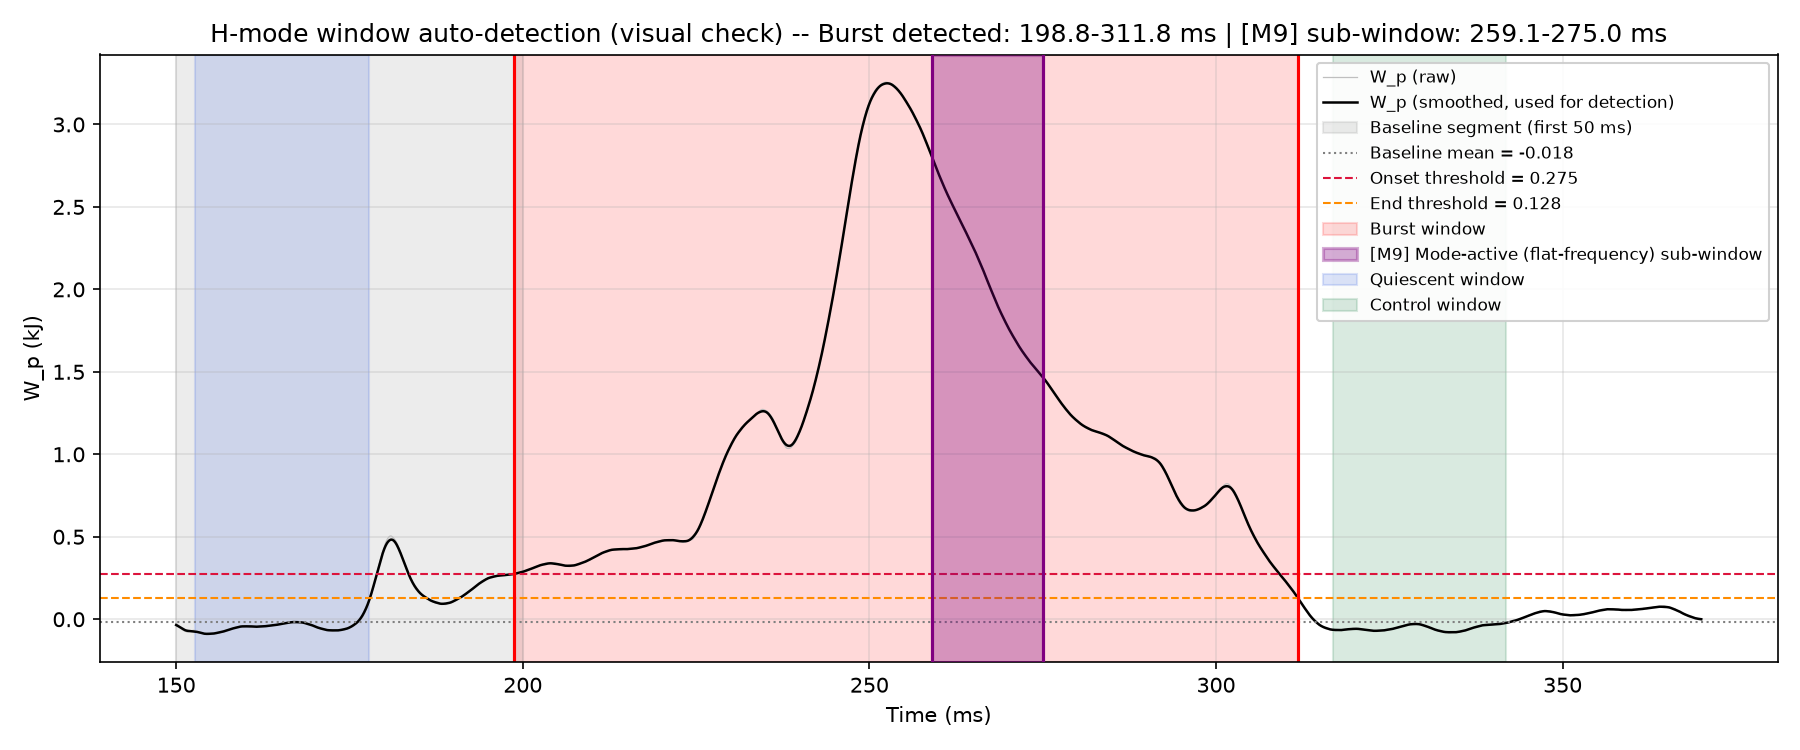
\includegraphics[width=\textwidth,height=0.8\textheight,keepaspectratio]{Images/obj3_nonlinear_coupling/mhd_burst_window_detection_88653.png}
    \end{figure}
\end{frame}

\begin{frame}{Backup: Objective 3 -- PSD Cross-Check of Leading Triads}
    \footnotesize
    A triad leg is ``PSD-confirmed'' if it lies within 1.5 bins ($\Delta f\approx\SI{0.98}{kHz}$,
    \texttt{nperseg=1024}) of a local PSD peak found via \texttt{scipy.signal.find\_peaks}.
    \vspace{0.15cm}
    \begin{center}
    \begin{tabular}{lccc}
        \toprule
        Triad (kHz) & $b^2$ & Leg offsets from nearest PSD peak (bins) & Verdict \\
        \midrule
        Headline: $98.6 - 48.8 = 49.8$ & 0.515 & $f_1$: 2.03, $f_2$: 0.97, $f_3$: 2.00 & \textbf{Not confirmed} \\
        Secondary: $89.8 - 41.0 = 48.8$ & 0.328 & $f_1$: 0.96, $f_2$: 0.98, $f_3$: 0.97 & \textbf{Confirmed} \\
        \bottomrule
    \end{tabular}
    \end{center}
    \vspace{0.2cm}
    \begin{itemize}
        \item The headline triad's own maximum ($b^2=0.515$) does not correspond to real
        spectral structure at $f_1$ or $f_3$ -- two of its three legs land ${\sim}2$ bins from the
        nearest genuine PSD peak.
        \item The secondary triad's $f_1=\SI{89.8}{kHz}$ coincides with the independently
        validated primary mode ($\sim\SI{89.0}{kHz}$), and all three legs are within 1 bin of
        confirmed peaks.
        \item Implication: the mathematically-largest bicoherence peak is not the most
        physically-grounded one. Reported here rather than silently substituted, since $b^2=0.515$
        remains the true maximum of the bicoherence surface.
    \end{itemize}
\end{frame}

\begin{frame}{Backup: Objective 3 -- Asymptotic Bias Scaling}
    \begin{figure}[h!]
        \centering
        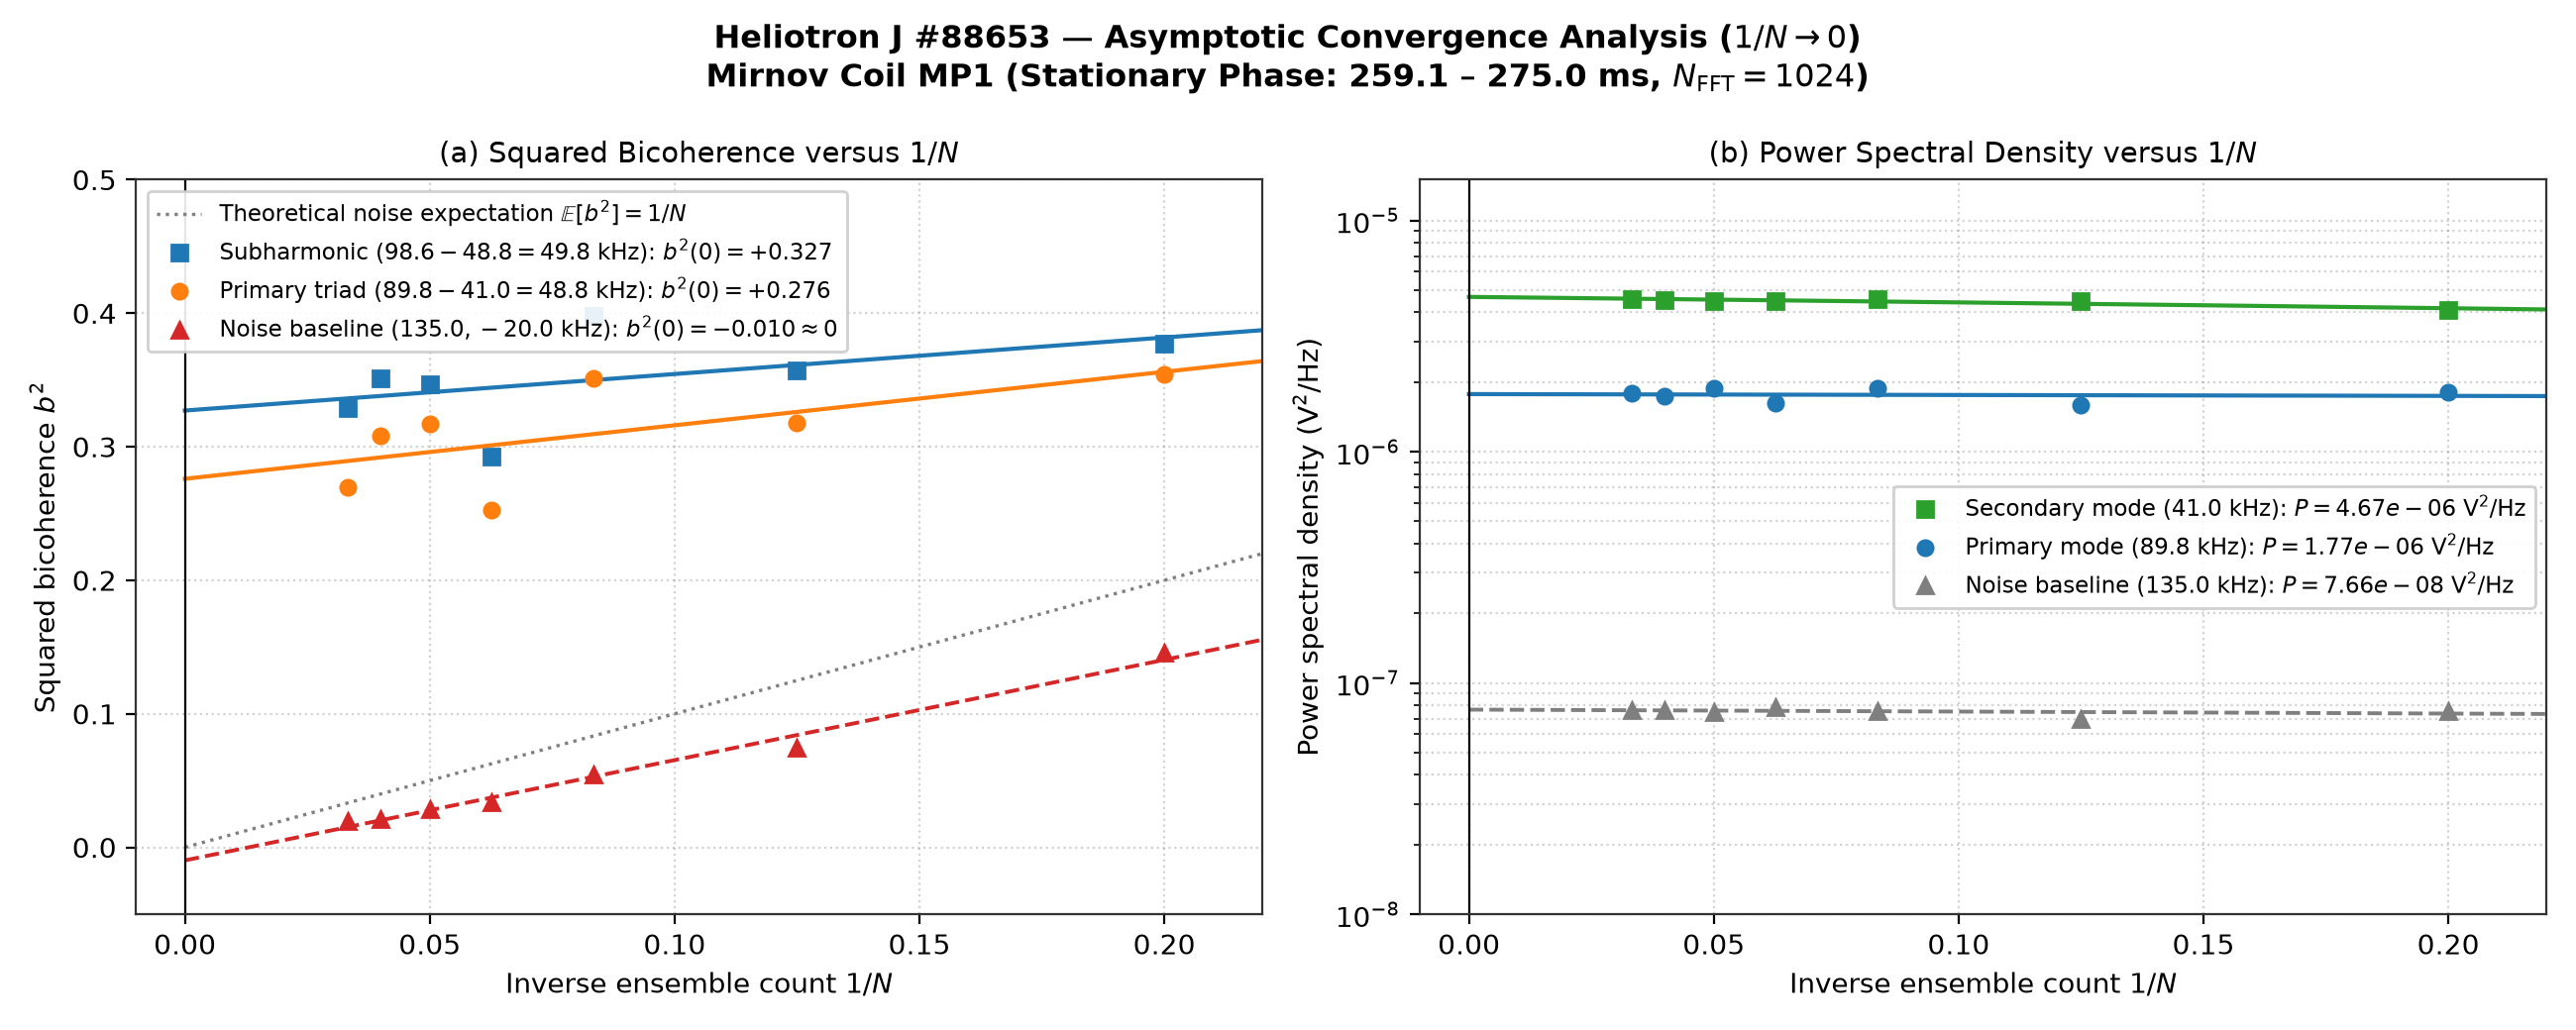
\includegraphics[width=\textwidth,height=0.8\textheight,keepaspectratio]{Images/obj3_nonlinear_coupling/mhd_asymptotic_bias_scaling_shot_88653.png}
    \end{figure}
\end{frame}

\begin{frame}{Backup: Objective 3 -- Statistical Nuance \& Energy Context}
    \textbf{Burst vs.\ Quiescent \& Control Comparisons}
    \begin{itemize}
        \item \textbf{Energy Transport:} the burst window shows elevated stored
        energy ($\langle W_p\rangle=\SI{2.07}{kJ}$) with a heavily degraded
        derivative ($\langle dW_p/dt\rangle=\SI{-83.24}{kJ/s}$).
        \item \textbf{Statistical inference:} 5.42\% of bins exceed $b^2>0.100$
        (the per-bin 95\% level for $N=30$; $0.20$ for $N_{\text{eff}}=15$) during
        the burst -- about the 5\% expected by chance.
        \item \textbf{Comparative nuance:} maximum $b^2$ is comparable in
        quiescent (0.3656) and control (0.4585) windows.
        \item \textbf{Conclusion:} the burst is not statistically superior to
        quiescent/control periods -- no rigorous basis to call this an
        exclusive H-mode signature.
    \end{itemize}
\end{frame}

\begin{frame}{Backup: Objective 3 -- Double-Validation Summary}
    \textbf{Reproducibility and Cross-Diagnostic Constraints}
    \begin{itemize}
        \item \textbf{Shot-to-shot reproducibility:} the coupling fails
        to reproduce on all channels (MP1, MP3, MP4) in validation shot
        \#88654 ($b^2\le0.34$ vs.\ \num{0.50} required) -- even though
        88654's primary mode structure closely mirrors 88653's (next
        backup slide).
        \item \textbf{Cross-diagnostic validation:} a scan of 36 Langmuir probe
        tips found zero tips exceeding $b^2>0.5$ matching a magnetic channel's
        leading triad.
        \item \textbf{Final result:} Objective 3 is \emph{not} validated
        under the strict double criterion.
    \end{itemize}
\end{frame}

\begin{frame}{Backup: Objective 3 -- Shot \#88654 Reproducibility Check}
    \footnotesize
    \textbf{Primary modes reproduce; the nonlinear coupling does not.}
    Same 259.1--275.0\,ms window, same dual-criterion pipeline, heating
    phase confirmed time-aligned (ECH off 291.2\,ms, NBI off
    300.4--300.6\,ms, identical in both shots).
    \vspace{0.15cm}
    \begin{center}
    \begin{tabular}{cccc}
        \toprule
        88653 $f$ (kHz) & 88654 $f$ (kHz) & Shift & $\gamma^2$ (88653 vs.\ 88654) \\
        \midrule
        40.0 & 37.5 & $-2.5$ & 0.97 vs.\ 0.96 \\
        89.0 & 87.0 & $-2.0$ & 0.85--0.94 vs.\ 0.90--0.96 \\
        45.5 & 43.0 & $-2.5$ & 0.92--0.95 vs.\ 0.85--0.92 \\
        83.5 & 82.5 & $-1.0$ & 0.61--0.82 vs.\ 0.69--0.86 \\
        79.0 & 77.0 & $-2.0$ & 0.43--0.76 vs.\ 0.66--0.89 \\
        \bottomrule
    \end{tabular}
    \end{center}
    \vspace{0.2cm}
    \begin{itemize}
        \item All five dual-criterion modes reproduce 1-to-1 (same rank
        order), downshifted 1--\SI{2.5}{kHz} (consistent with $I_p$
        $\sim$5\% lower in 88654) with comparable or higher inter-probe
        coherence.
        \item Despite this, bicoherence at the PSD-confirmed triad
        (89.8/\SI{41.0}{kHz}) stays at $b^2\le0.34$ in 88654 on every
        channel -- well below the \num{0.50} threshold that 88653 itself
        clears.
        \item The modes are robustly present; the three-wave coupling
        between them is not reproduced.
    \end{itemize}
\end{frame}

\begin{frame}{Backup: Objective 3 Comparative -- Bicoherence Matrices}
    \begin{columns}[T]
        \begin{column}{0.5\textwidth}
            \centering ECH+NBI\\
            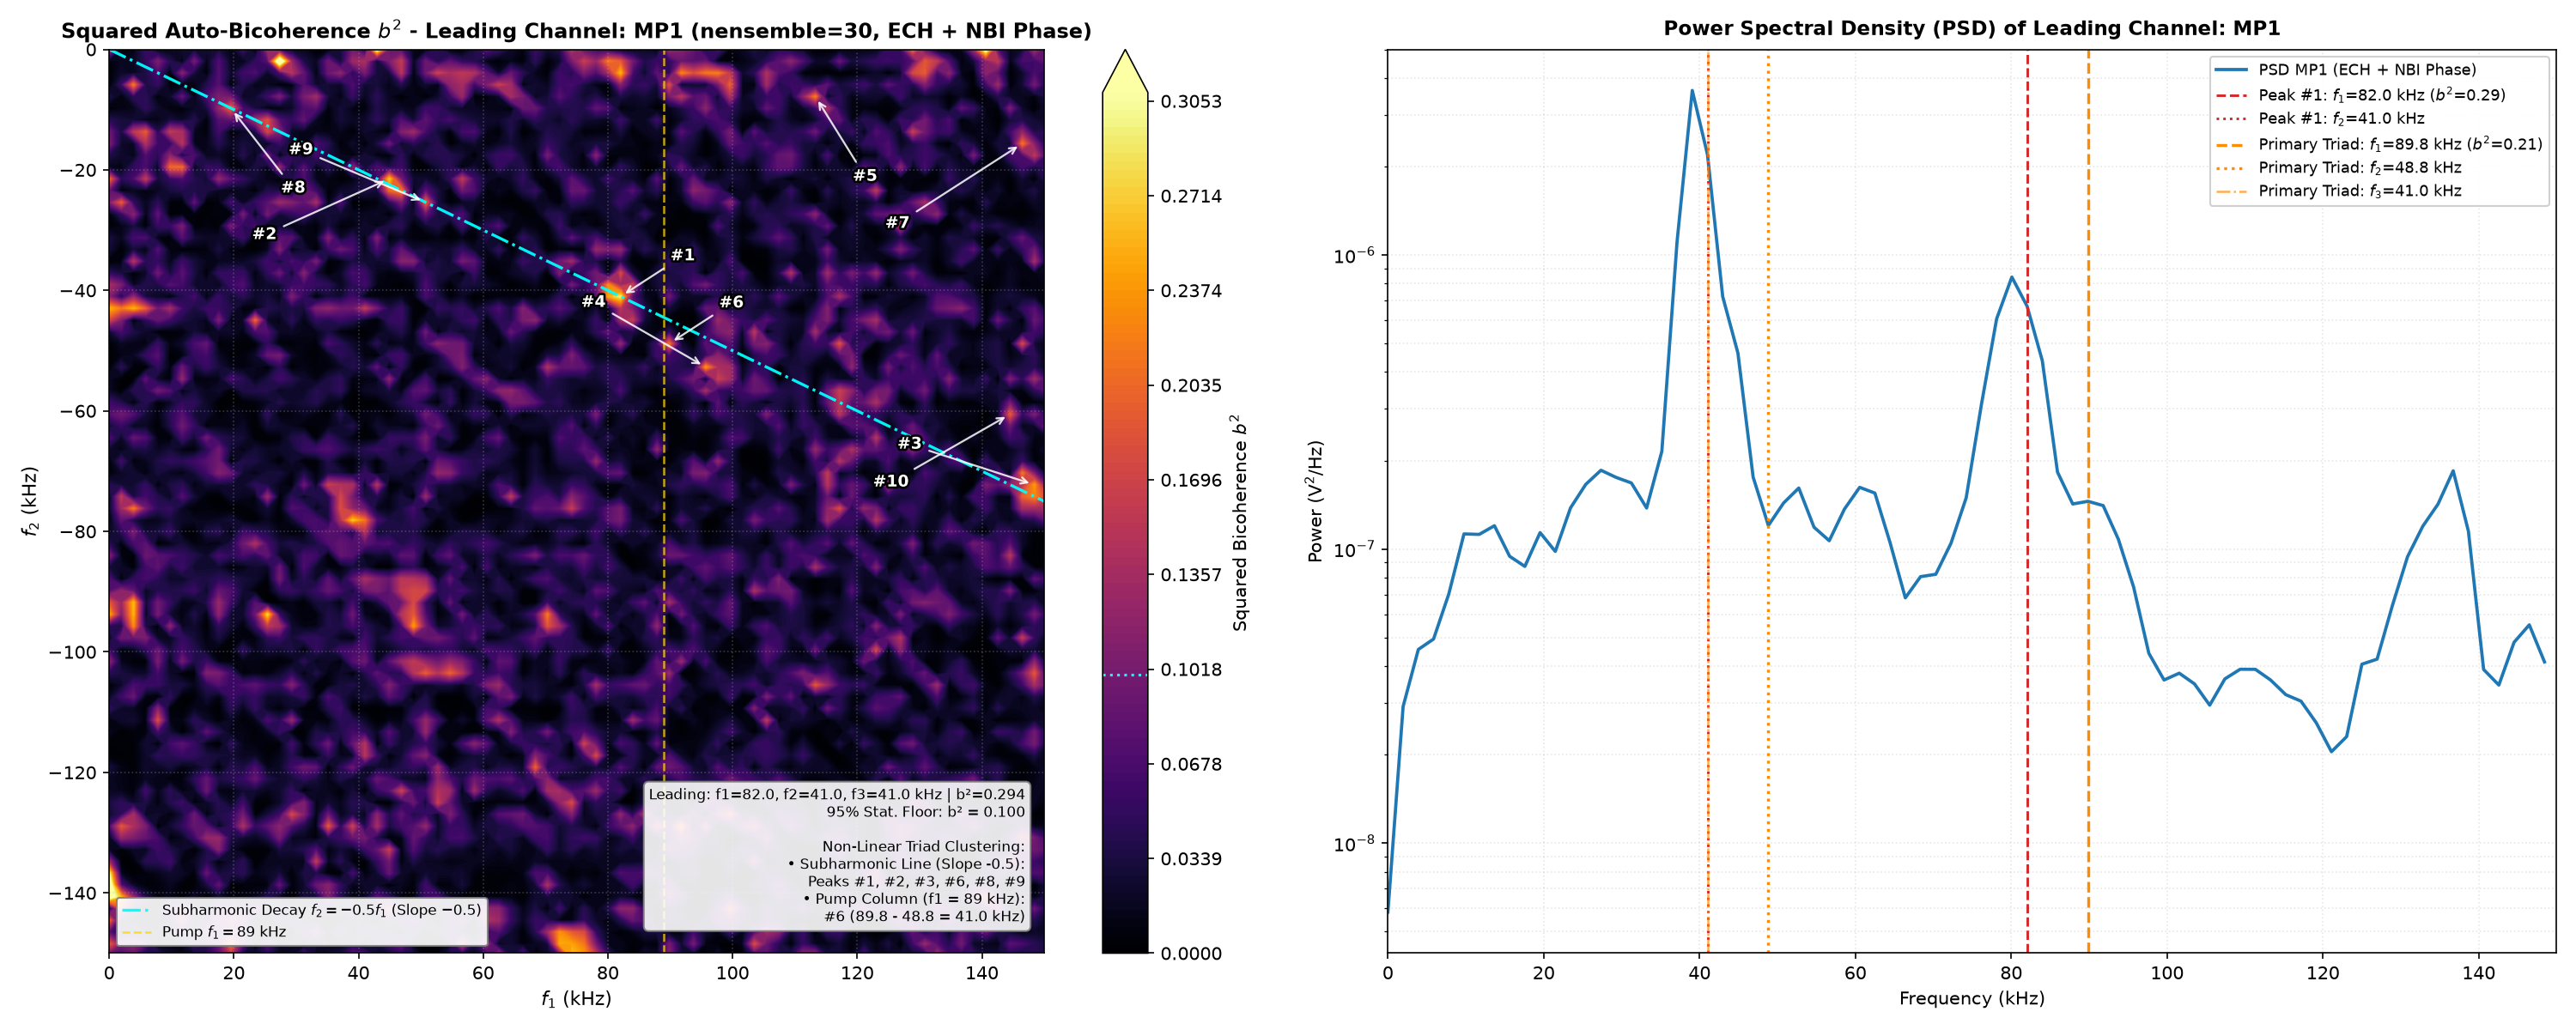
\includegraphics[width=\textwidth]{Images/heating_phase_comparison/mhd_bicoherence_objective3_88653_ECH_NBI.png}
        \end{column}
        \begin{column}{0.5\textwidth}
            \centering NBI-only\\
            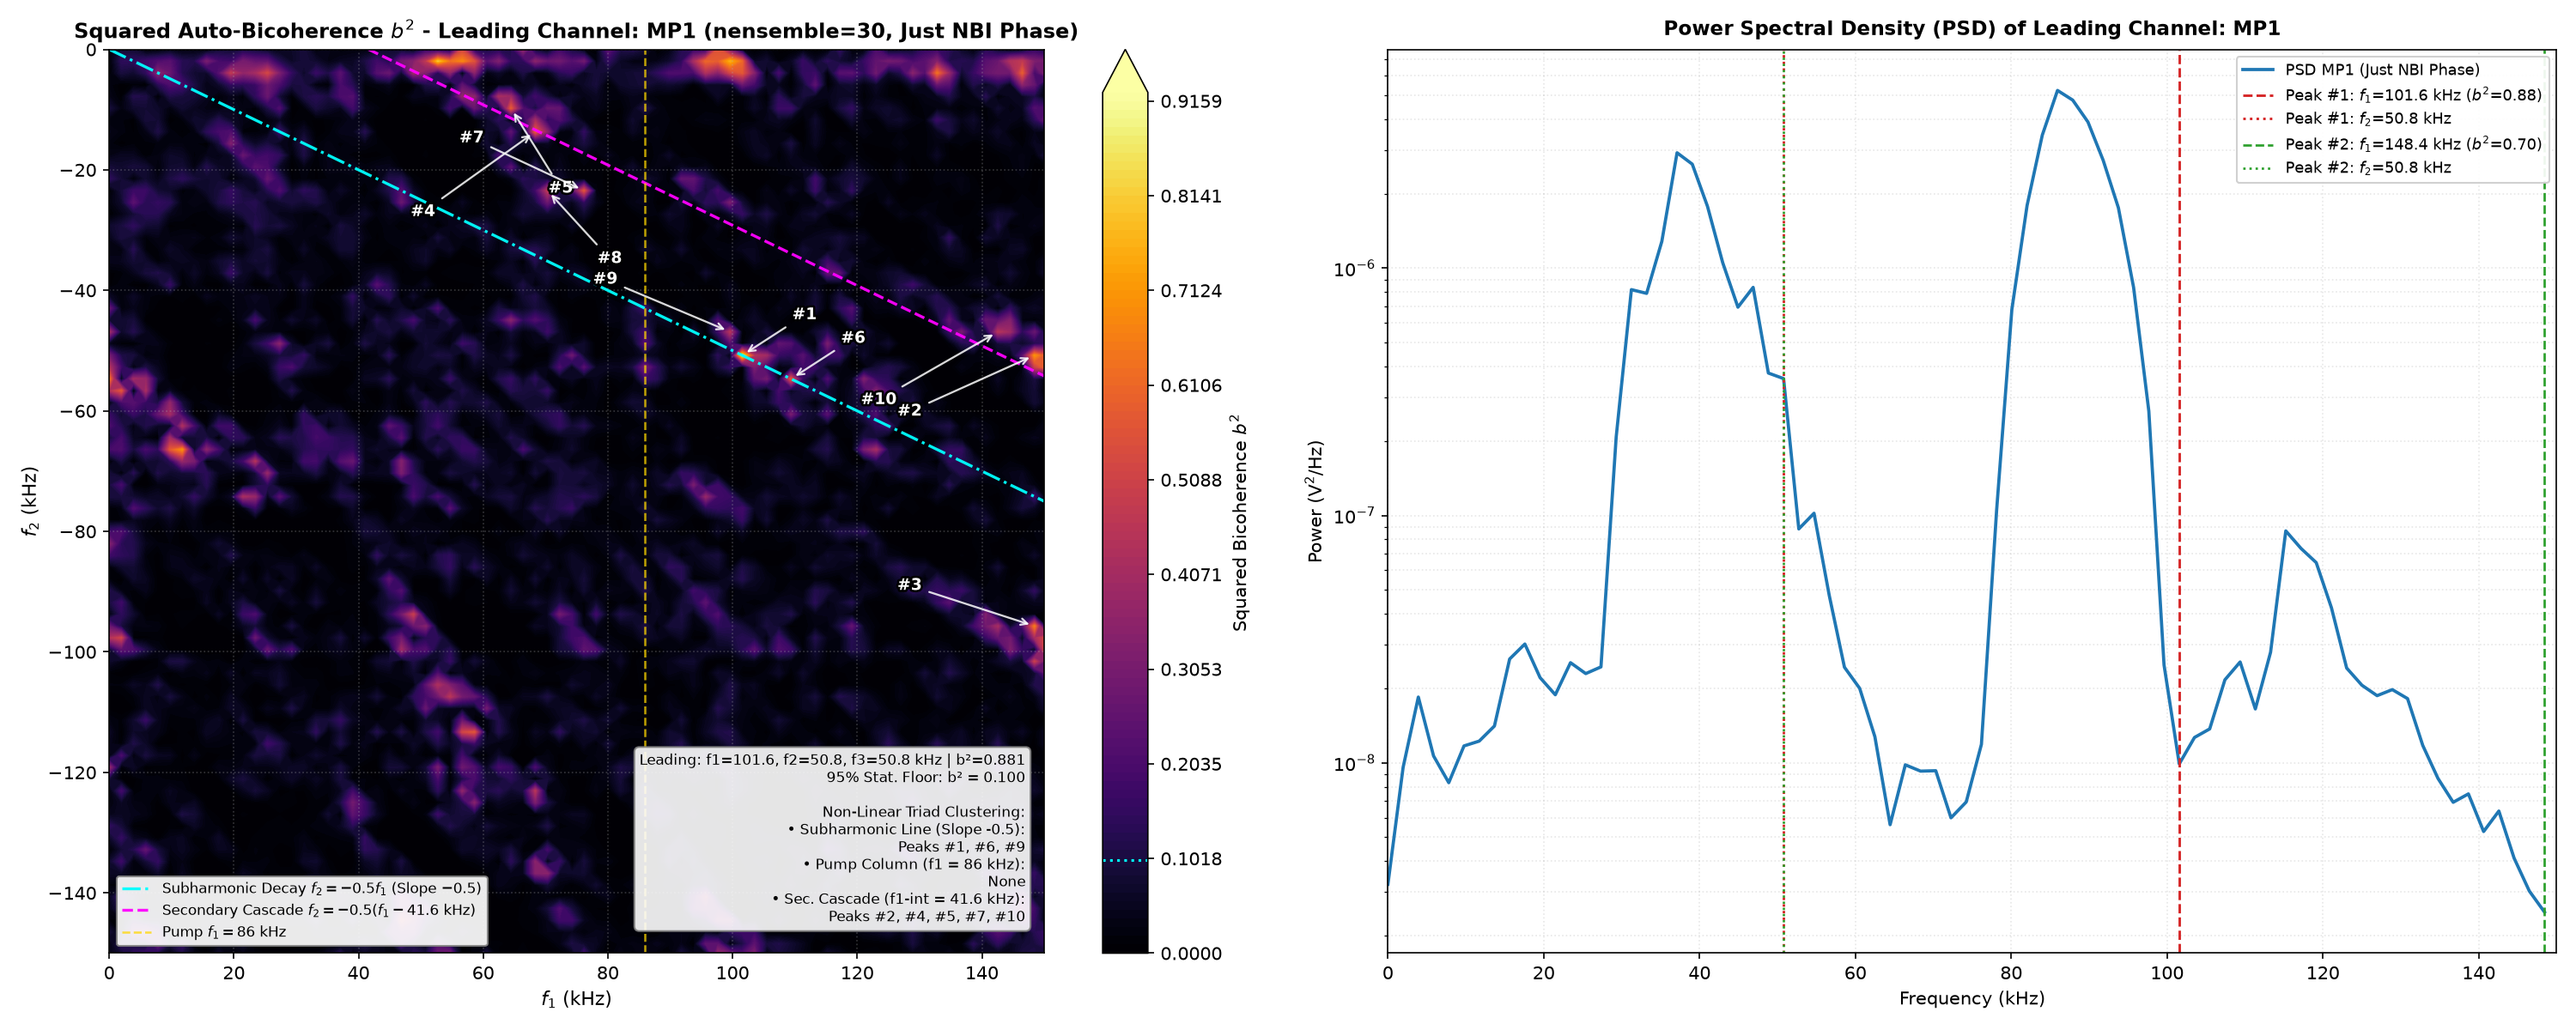
\includegraphics[width=\textwidth]{Images/heating_phase_comparison/mhd_bicoherence_objective3_88653_NBI_only.png}
        \end{column}
    \end{columns}
\end{frame}

\begin{frame}{Backup: Objective 3 Comparative -- Leading Bicoherence Triads}
    \small
    \centering
    \begin{tabular}{lcc}
        \toprule
        Window & Triad $f_1 - f_2 = f_3$ (kHz) & $b^2$ \\
        \midrule
        ECH+NBI  & $82.0 - 41.0 = 41.0$   & 0.2937 \\
        ECH+NBI  & $44.9 - 21.5 = 23.4$   & 0.2660 \\
        ECH+NBI  & $148.4 - 72.3 = 76.2$  & 0.2381 \\
        \midrule
        NBI-only & $101.6 - 50.8 = 50.8$  & \textbf{0.8811} \\
        NBI-only & $148.4 - 50.8 = 97.7$  & 0.6962 \\
        NBI-only & $148.4 - 95.7 = 52.7$  & 0.6517 \\
        \bottomrule
    \end{tabular}
    \vspace{0.3cm}
    \normalsize
    Leading NBI-only triads reach $b^2$ up to $\sim$3$\times$ higher than the
    strongest ECH+NBI triads -- statistically significant, but the same
    double-validation caution applies.
\end{frame}

\end{document}
